% UNINA MSc thesis template (extbook, 12pt, oneside) carrying this thesis's own
% figure, algorithm and notation setup.
\documentclass[a4paper, 12pt, oneside]{extbook}
\usepackage[T1]{fontenc}
\usepackage[utf8]{inputenc}
\usepackage[english]{babel}
\usepackage{lmodern}
\usepackage{courier}

\usepackage{geometry}
\newgeometry{
left=   1.5 in,
bottom= 1.5 in,
right=  1 in,
top=    1 in
}

% Running header: current chapter left, current section right.
\usepackage{fancyhdr}
\setlength\headheight{14pt}
\pagestyle{fancy}
\fancyhf{}
\lhead{\footnotesize\nouppercase{\leftmark}}
\rhead{}
\renewcommand{\sectionmark}[1]{\markright{\thesection\quad #1}}
\cfoot{\thepage}
\renewcommand{\headrulewidth}{0.4pt}

\usepackage{setspace}
\singlespacing

% Grafica
\usepackage{graphicx}
\graphicspath{{figures/}{img/}}
\usepackage{microtype}

% Package usati per il frontespizio
\usepackage{tikz}
\usetikzlibrary{positioning,arrows.meta,fit,backgrounds,shapes.geometric,calc}

\usepackage{amsmath,amssymb}
\usepackage{booktabs}
\usepackage{subcaption}
\captionsetup[subfigure]{font=scriptsize,labelfont=bf,skip=1.5pt}
\usepackage[section]{placeins}
\usepackage{tabularx}
\newcolumntype{L}{>{\raggedright\arraybackslash}X}
\usepackage{enumitem}
\usepackage{titlesec}
\usepackage[ruled,vlined]{algorithm2e}
\SetKwComment{Comment}{$\triangleright$\ }{}
\usepackage{cite}

\titlespacing*{\section}{0pt}{2.5ex plus 0.5ex minus 0.3ex}{0.9ex plus 0.2ex}
\titlespacing*{\subsection}{0pt}{1.3ex plus 0.3ex minus 0.2ex}{0.8ex plus 0.2ex}

\setlength{\parskip}{0pt}

% Long inline formulas give TeX few break points in a 14pt narrow measure;
% this lets it stretch a line rather than bleed into the margin.
\setlength{\emergencystretch}{3em}

\newcommand{\qdot}{\dot{q}}
\newcommand{\todocite}[1]{\textcolor{red}{[REF NEEDED: #1]}}

% Same R/L and per-joint colours as the MATLAB hardware-trial panels (fig_thesis_hw.m).
\definecolor{hwred}{rgb}{0.753,0.224,0.169}
\definecolor{hwblue}{rgb}{0.133,0.333,0.643}
\definecolor{hwj1}{rgb}{0.000,0.447,0.698}
\definecolor{hwj2}{rgb}{0.835,0.369,0.000}
\definecolor{hwj3}{rgb}{0.000,0.620,0.451}
\definecolor{hwj4}{rgb}{0.800,0.475,0.655}
\definecolor{hwj5}{rgb}{0.902,0.624,0.000}
\definecolor{hwj6}{rgb}{0.337,0.706,0.914}
\definecolor{hwj7}{rgb}{0.000,0.000,0.000}
\definecolor{hwshade}{rgb}{0.995,0.968,0.829}
% One shared R/L legend, set once ahead of a multi-panel hardware figure
% instead of repeating it in every panel.
\newcommand{\hwrllegend}{%
  \centering
  {\footnotesize\textcolor{hwred}{\rule[0.25em]{0.9em}{1.1pt}}~Right \quad \textcolor{hwblue}{\rule[0.25em]{0.9em}{1.1pt}}~Left}\par\vspace{0.3em}%
}
% One shared J1..J7 legend for a joint-space figure.
\newcommand{\hwjointlegend}{%
  \centering
  {\footnotesize
   \textcolor{hwj1}{\rule[0.25em]{0.9em}{1.1pt}}~J1 \quad
   \textcolor{hwj2}{\rule[0.25em]{0.9em}{1.1pt}}~J2 \quad
   \textcolor{hwj3}{\rule[0.25em]{0.9em}{1.1pt}}~J3 \quad
   \textcolor{hwj4}{\rule[0.25em]{0.9em}{1.1pt}}~J4 \quad
   \textcolor{hwj5}{\rule[0.25em]{0.9em}{1.1pt}}~J5 \quad
   \textcolor{hwj6}{\rule[0.25em]{0.9em}{1.1pt}}~J6 \quad
   \textcolor{hwj7}{\rule[0.25em]{0.9em}{1.1pt}}~J7}\par\vspace{0.3em}%
}
\newcommand{\hwxyzlegend}{%
  \centering
  {\footnotesize
   \textcolor{hwj1}{\rule[0.25em]{0.9em}{1.1pt}}~$x$ \quad
   \textcolor{hwj2}{\rule[0.25em]{0.9em}{1.1pt}}~$y$ \quad
   \textcolor{hwj3}{\rule[0.25em]{0.9em}{1.1pt}}~$z$ \qquad
   \textcolor{hwshade}{\rule[0.05em]{1.4em}{0.9em}}~operator in control}\par\vspace{0.3em}%
}

\usepackage[bookmarks]{hyperref}
\hypersetup{colorlinks=true,linkcolor=black,citecolor=black,urlcolor=blue,
  pdftitle={Adaptive Human-Robot Shared Autonomy Based on Safety-Aware Control: A Validation Case in Bimanual Manipulation With the TRIAGo Robotic Platform},
  pdfauthor={Roberto Rocco}}

\begin{document}

\begin{titlepage}
\thispagestyle{empty}
\raggedright % Allinea a sinistra

\begin{tikzpicture}
\node[anchor=south west] at (4,0) {
\includegraphics[scale=0.75]{img/logo/logo_copertina_1}};
\node[anchor=south west] at (0,1.5) {
\includegraphics{img/logo/logo_copertina_2}};
\node[anchor=south west] at (0,0.5) {\textsf{Scuola Politecnica e delle Scienze di Base}};
\node[anchor=south west] at (0,0) {\textsf{Corso di Laurea Magistrale in Ingegneria dell'Automazione e Robotica}};
\end{tikzpicture}

\vfill

{\large Tesi di Laurea Magistrale in Ingegneria dell'Automazione e Robotica}
\\[1cm]
\begin{spacing}{1.8}
{\textbf{\textit{\LARGE Adaptive Human--Robot Shared Autonomy Based on Safety-Aware Control: A Validation Case in Bimanual Manipulation With the TRIAGo Robotic Platform}}}
\end{spacing}
\vspace{1cm}

{\large Anno Accademico 2025/2026}

\vfill


\begin{table}[h]
Relatore
\\
\textbf{Ch.mo prof.\ Mario Selvaggio}
\\
\textbf{Marco Ferro}
\\
\textbf{Claudio Pacchierotti}
\\ \\
{\raggedright Candidato}
\\
\textbf{Roberto Rocco}
\\
\textbf{matr.\ P38000274}
\end{table}

\end{titlepage}

\frontmatter

\chapter{Abstract}

\noindent Driving a two-armed robot from a distance, through a single hand-held haptic interface, is difficult for reasons that are structural rather than incidental. The operator perceives the workcell only through the robot, commands one arm at a time through a device whose workspace is a fraction of the robot's, and must keep both arms clear of the environment and of each other while doing so. Assistance can relieve part of that load: a layer that infers which object the operator is reaching for can steer the arm toward it and can push the operator's hand toward it through the device. The difficulty is that assistance which is confidently wrong is worse than no assistance at all, and assistance that overrides the operator removes exactly the judgement the operator was present to supply.

This thesis addresses that trade-off by separating what the robot can decide from what only the operator can. A reactive layer computes, at every instant, the best locally admissible motion toward each candidate goal, and enforces collision avoidance and joint limits as hard constraints of a nominal barrier condition on whatever command finally reaches the arms, so that no assistance and no operator input can produce an unsafe motion. That layer is deliberately local, and its locality is what defines the division of labour: it cannot know which of several objects is intended, which side of an obstacle to pass, or when a temporary detour away from the goal is the only way out of a dead end. Those decisions remain with the operator. Assistance is therefore arbitrated on agreement --- it contributes while the operator is moving with it, and withdraws as soon as the operator moves against it --- so the robot supplies precision and safety while the operator supplies intent and judgement.

The architecture was implemented on a bimanual mobile manipulator and validated end to end on the physical robot, from camera-perceived obstacle geometry through teleoperated grasping under barrier-enforced collision avoidance. The evaluation crossing the two classical teleoperation mappings --- position control with indexing and spring-centred rate control --- with three assistance strategies --- haptic guidance, autonomous blending of the operator's command with the inferred policy, and both together --- over two tasks that differ in whether they force the two arms to cooperate, was run with human participants in a matched simulation environment.

Across the factorial comparison, the assistance strategy, not the motion mapping, is what moves objective performance: reference blending is what shortens the task and steadies the hand, force guidance alone is consistently the weakest condition in both mappings, and no significant difference was found between blending alone and blending with guidance. The minimum clearance recorded shows no significant difference across conditions, consistent with the barrier, rather than the operator or the assistance, setting that floor. Participants agree with that objective picture only in part: they rate the blended conditions as more controllable and more trustworthy than guidance alone, even though blending is exactly the channel that takes some authority away from the hand, while the choice of motion mapping, despite separating the two objectively, is something participants report noticing hardly at all. On the physical robot, the same controller and arbitration carried a real teleoperated grasp to completion and, on a second attempt, recorded the architecture's one safety violation, when a clearance-blind retreat re-armed a deliberately suspended collision barrier onto an unresolved overlap before the operator stopped the robot; that single case does not settle how the architecture behaves at hardware scale, and is treated here as a limitation rather than as a conclusion.


\tableofcontents
\listoffigures
\listoftables

\mainmatter
\rhead{\footnotesize\nouppercase{\rightmark}}

\chapter{Introduction}
\label{ch:intro}

\section{Motivation}
\label{sec:motivation}

A manipulator teleoperated through a single grounded haptic interface --- a device whose handle is mechanically fixed to the desk rather than carried freely in the hand, the very property that lets it render forces back onto the operator --- is used precisely where full autonomy is not yet trusted, or not yet possible, and where a remote operator's judgement must still resolve which of several objects to reach for, which side of an obstacle to pass, and when a task-level decision is required that no perception pipeline is asked to make~\cite{jain2020probabilistic}. Bilateral teleoperation architectures close this loop in both directions, forwarding the operator's motion to the manipulator and rendering the resulting interaction back to the operator's hand~\cite{hokayem2006bilateral}. The interface itself imposes a structural asymmetry, established by Kim et al.'s comparison of the two dominant motion mappings~\cite{kim1987comparison}: its own workspace is a fraction of the manipulator's reach, so a position-controlled mapping requires the operator to periodically disengage and reposition the handle, while a rate-controlled mapping removes that limitation at the cost of a less intuitive, integrating relationship between hand and end-effector. Extending such a single-handed interface to a bimanual manipulator multiplies both the coordination and the risk: the operator drives one arm at a time through the one channel available, while both arms must remain clear of the environment and of each other throughout.

Shared autonomy relieves part of this load by inferring, from the operator's own command, which of several candidate goals is intended, and by combining an autonomous policy toward that goal with the operator's raw input~\cite{selvaggio2021autonomy,losey2018review}. Safety, in the sense used throughout this thesis, means that the motion actually commanded to the arms satisfies hard constraints at every control tick --- no collision with the modelled obstacles, including the two arms against each other and against themselves, and joint position and velocity limits respected. The canonical realization of shared autonomy is a convex blend of the two commands, weighted by an estimate of confidence in the inferred goal~\cite{dragan2013policy}. Such a blend does not, by itself, respect any constraint that the operator's command and the autonomous policy each individually satisfy: once the admissible set is nonconvex, as it generically is around real obstacle geometry, a blend of two individually safe commands can violate a constraint that neither command violates on its own, shown formally by Chaubey et al. and empirically by Guler et al.~\cite{chaubey2026minimalintervention,guler2026barrierik}. Confidently wrong assistance is worse than none: a blend that is safe only in expectation, and not enforced to be safe at the instant it is executed, can still drive an arm into contact.

A hard constraint applied after arbitration, rather than a soft penalty folded into the blend objective, is the response this literature converges on, most often realized as a control barrier function (CBF) embedded in a quadratic program (QP) solved at every control tick~\cite{ames2017cbf}. Published realizations of this post-arbitration principle remain partial: the closest, Guler et al.'s filtered pipeline, is validated only in simulation and a virtual-reality study, inside a position-space inverse-kinematics solve rather than a joint-velocity QP; the closest use of the filter's own dual variables as operator feedback, Raphalen et al.'s, is demonstrated around a single arm and without arbitration against an inferred autonomous policy~\cite{raphalen2026feeling}. No published system realizes a post-arbitration hard-safety filter, natively formulated at the joint-velocity level, on a physical bimanual manipulator, nor uses that filter's own shadow prices for anything beyond a one-way feedback channel.

This thesis addresses that combination directly: a strictly convex control-Lyapunov-function (CLF)--CBF QP enforces collision avoidance and joint limits as hard constraints of a nominal barrier condition on the command that finally reaches each arm, after an alignment-based arbitration law has already combined the operator's instantaneous twist with a belief-weighted autonomous policy. The controller and the perception pipeline supplying its collision geometry are validated end to end on a physical bimanual platform; the factorial comparison across teleoperation mappings and assistance strategies is then run at human-subject-study scale in a matched simulation environment.

\section{Research questions and hypotheses}
\label{sec:rqs}

The motivation above resolves into six research questions.

\begin{enumerate}[nosep, label=\textbf{RQ\arabic*.}]
\item (safety) Does the post-arbitration filter enforce its nominal barrier condition on physical hardware, and where does the sampled, physical closed loop depart from that condition?
\item (assistance channel) Which assistance channel, force guidance or reference blending, drives objective performance and subjective experience, and does combining both change either?
\item (motion mapping) Does the choice of teleoperation mapping interact with the assistance channel on objective and subjective measures?
\item (arbitration) Does alignment-based arbitration preserve operator primacy while still assisting?
\item (adaptive scheduling) Does reusing the QP's own shadow price to schedule tracking slack behave as intended when exercised on hardware?
\item (grasp-object barrier management) Does the hybrid grasp lifecycle move a target object into and out of the collision model without a detectable safety cost?
\end{enumerate}

A human-subject study tests RQ2 and RQ3 against four hypotheses, formed before any trial is run and stated here on named measures so that each is falsifiable against a quantity rather than an unstated notion of merit.

\begin{enumerate}[nosep, label=\textbf{H\arabic*.}]
\item (channel--mapping interaction) H1 predicts an interaction rather than one channel dominating: force guidance outperforms reference blending on task time $T$~\eqref{eq:mT} under the clutch mapping, and reference blending outperforms force guidance under the joystick mapping. The clutch-side half rests on a system-specific conjecture --- no prior source evaluates haptic guidance as a substitute for depth perception --- that a force pulling the handle toward the goal, with the handle visibly following it, compensates for the depth cues the rear-facing view denies the operator. The joystick-side half follows a channel-congruence argument instead: a guidance force adds to the effort of holding a direction or speed against the mapping's own centring spring, whereas reference blending arbitrates directly on the same velocity command the joystick already issues, so the two channels are expected to compete for authority under one mapping and to reinforce each other under the other, consistent with Abbink, Mulder, and Boer's principle that assistance should bias, never replace, the operator's own input~\cite{abbink2012hapticshared}.
\item (mapping) H2 predicts that the clutch mapping yields the shorter task time $T$ and path length $L$~\eqref{eq:mL}, and the same direction on the subjective composite index $\bar{S}$: the one-to-one correspondence between hand motion and gripper motion is expected to outweigh the cost of the re-indexing it requires --- itself guided in time by the joint-limit vibrotactile cue and in orientation by the alignment torque~\eqref{eq:aligntorque} --- against the joystick mapping's indirect, rate-controlled correspondence.
\item (authority cost of blending) H3 predicts that reference blending is rated \emph{worse} than force guidance alone on the workload subscales for mental and physical demand, $S_{\mathrm{md}}$ and $S_{\mathrm{pd}}$: a reference that no longer moves exactly as commanded registers as effort spent resisting or correcting it, an authority cost of the kind Zhang, Tron, and Khurshid identify wherever a felt intervention alters an operator's command rather than merely reporting it~\cite{zhang2021hapticagreement}. This effect is expected to be sharpest in the more cluttered relay scenario, where the belief-weighted policy's own safety margin can pull the blended reference away from an operator command that holds alignment on one task component, orientation for instance, while intending to pass closer to an obstacle than the policy allows; this scenario-specific half is noted for completeness, since the design averages the two scenarios into one value per condition and cannot test it.
\item (quality over speed) H4 predicts that, because a blended reference is one the safety filter can execute rather than one it must partially refuse, blending lowers path length $L$, mean tracking slack $\bar{\delta}$~\eqref{eq:mdelta}, and filter active time $T_{\lambda}$~\eqref{eq:mTlam} relative to force guidance alone, with no predicted direction on task time $T$, since nothing in the mechanism ties the size of the correction to the speed at which the operator reaches the goal.
\end{enumerate}

RQ4 through RQ6 are addressed by implementation and by exercise on physical hardware, not by a controlled experiment, and carry no tested hypothesis.

\section{Contributions}
\label{sec:contributions}

\begin{itemize}[nosep]
\item \textbf{A shared-autonomy framework combining autonomous grasping, a post-arbitration safety filter, haptic feedback, and command blending.} A strictly convex CLF--CBF QP, solved at the velocity-level inverse-kinematics (IK) stage with a CLF task-tracking constraint and a CBF collision constraint aggregated over the closest obstacle pairs by a soft minimum, enforces collision avoidance and joint limits on the already-arbitrated command reaching each arm. Authority given to the autonomous policy is arbitrated on the instantaneous directional agreement between the operator's commanded twist and the goal-directed policy's own twist, computed from a discounted belief score over candidate goals rather than a scalar confidence, distance, or entropy summary, and ramps to zero exactly when the two conflict, so the operator retains sole authority over any motion it opposes. The safety filter's own dual variables, already computed at every solve, are used as the robot's self-assessment of how constrained its surroundings are, and are low-pass filtered and fed back into the QP's own cost to schedule its per-arm tracking slack: tracking tightens in free space and yields near an active constraint, so precision and execution time are given up only where safety requires it, closing this loop internally rather than only rendering the multiplier to the operator as a feedback force. The same signal also drives, in development runs outside the reported evaluation, the time scaling of assigned trajectories, and opens the scheduling of the CLF convergence rate and of the posture weight. A grasped object is treated as a hybrid, not a continuously invariant, barrier: the target leaves and rejoins the declared obstacle pair set through explicit regimes --- exclusion during the blind approach, relaxed-margin contact during closure, re-parenting into the protected chain, and ramped reactivation on release --- each with its own reset map and switching condition, with continuity claimed only for the margin parameter within a regime, not for invariance of the original obstacle set across regimes.
\item \textbf{Deployment of the framework on physical bimanual hardware and in a matched simulation environment.} The controller and the camera-based perception pipeline supplying its collision geometry are validated end to end on a physical bimanual mobile manipulator, from camera-perceived obstacle geometry through teleoperated grasping under barrier-enforced collision avoidance. The same architecture also runs in a matched simulation environment built to exercise the framework at human-subject-study scale.
\item \textbf{A factorial human-subject study for validation.} The evaluation crosses both classical teleoperation mappings, position control with indexing and spring-centred rate control, with the assistance strategies above, over two scenarios that differ in whether they force the two arms to cooperate, run by human participants to test the framework's objective and subjective effect.
\end{itemize}

\section{Thesis outline}
\label{sec:outline}

The remainder of this thesis is organized as follows. Chapter~\ref{ch:sota} reviews the four literatures this thesis draws on --- teleoperation of remote manipulators, shared control and shared autonomy, safety-critical control, and perception for safety-critical control --- and closes by positioning the contributions above against the closest prior systems (Section~\ref{sec:sota-positioning}). Chapter~\ref{ch:method} develops the methodology: the QP-CLF-CBF safety controller (Section~\ref{sec:qp}), the shared-autonomy belief estimator and alignment-based arbitration (Section~\ref{sec:sa}), the grasp lifecycle and world-model maintenance (Section~\ref{sec:grasp}), and the haptic interface and force rendering (Section~\ref{sec:teleop}). Chapter~\ref{ch:exp} validates the architecture on physical hardware (Section~\ref{sec:hwvalidation}), describes the setup of the user study (Section~\ref{sec:study}), and reports the results of the human-subject study. Chapter~\ref{ch:discussion} reads those results against the hypotheses of Section~\ref{sec:rqs}, weighs alternative explanations, and states threats to validity. Chapter~\ref{ch:conclusions} synthesises the whole, states the architecture's limitations, and outlines directions for future work; Appendix~\ref{app:config} collects every configuration parameter referenced throughout.

\chapter{State of the art}
\label{ch:sota}

This thesis sits at the intersection of four literatures rarely brought together in one system: teleoperation of remote manipulators, where an operator commands a robot arm through a haptic or kinematic interface; shared control and shared autonomy, where an inferred estimate of operator intent contributes to the command actually executed; safety-critical control, where control barrier functions (CBFs) realized inside a quadratic program (QP) keep the commanded motion inside a collision-free set by formal guarantee rather than heuristic penalty; and perception for safety-critical control, where the obstacle geometry that safety layer relies on is measured by the robot's own camera rather than given to it beforehand. Each field is mature on its own. What this chapter argues, and what Section~\ref{sec:sota-positioning} makes explicit against the closest prior system, is that their intersection --- safety enforced strictly after arbitration, on real hardware, with the safety filter's own dual variables closing the loop back to both controller and operator --- remains sparsely populated. Section~\ref{sec:sota-teleoperation} reviews bilateral teleoperation and the motion mappings this thesis treats as a factor of its user study. Section~\ref{sec:sota-shared-control} surveys shared autonomy from intent inference to arbitration and isolates the failure mode of linear blending that motivates the rest of the chapter. Section~\ref{sec:sota-haptic-fixtures} covers haptic shared control as a mechanism for making assistance felt rather than only computed. Section~\ref{sec:sota-safety-critical} is the technical core, tracing control barrier functions from potential fields to unified control-Lyapunov-function--control-barrier-function quadratic programs and their use inside the teleoperation loop. Section~\ref{sec:sota-perception} reviews the perception pipelines that build the obstacle model such a controller consumes. Section~\ref{sec:sota-positioning} closes the chapter by positioning this thesis's contribution against the reviewed work.

\section{Teleoperation of remote manipulators}
\label{sec:sota-teleoperation}

Bilateral teleoperation closes the loop between operator and remote manipulator in both directions: the operator's motion drives the robot, and a force computed from the robot's interaction with its environment is rendered back to the operator's hand. Hokayem and Spong survey a century's worth of architectures for this loop, from simple position--position and force--position schemes to four-channel architectures that pass both position and force information in each direction~\cite{hokayem2006bilateral}. The central difficulty, established in Lawrence's two-port formulation, is that transparency (the rendered impedance matching the true remote impedance) and stability trade against each other whenever the channel introduces delay or the haptic display has finite bandwidth~\cite{lawrence1993stability}.

\label{sec:sota-mappings}
\begin{sloppypar}
A teleoperation interface maps the operator's hand motion, bounded by the haptic device's own workspace, onto the larger and differently shaped workspace of the remote manipulator. Two mappings dominate the literature, and Kim, Tendick, Ellis, and Stark's comparison remains the reference study establishing that they are not interchangeable~\cite{kim1987comparison}. In position control, the handle pose maps directly to a desired remote pose; because the device workspace is smaller than the manipulator's reach, position control requires indexing, also called clutching --- the operator periodically disengages the mapping, repositions the handle, and re-engages --- trading continuous correspondence for an added motor step at every indexing event. In rate control, handle displacement from a centred rest pose maps to a commanded remote velocity, removing the workspace-mismatch problem at the cost of an integrating hand-to-end-effector relationship generally found less intuitive for fine positioning. Kim et al. found rate control to dominate once the manipulator's dynamics differ substantially from the hand's own, and position control to dominate when the two are kinematically similar and indexing cost is low~\cite{kim1987comparison}. The distinction reaches deeper than ergonomics: zero handle displacement means something different in each mapping. In rate control it commands zero remote velocity, a natural rest state; in position control with indexing it can mean the handle is disengaged and moving freely while the remote arm holds still, so the same physical handle state carries opposite consequences for what the robot is doing. This asymmetry is why this thesis treats the choice of motion mapping as a factor of the user study rather than a fixed implementation decision.
\end{sloppypar}

Both mappings face a further problem specific to the wrist: a device's rotational workspace is typically smaller and differently shaped than the manipulator's, so the operator's and the end-effector's orientations drift apart unless something keeps them linked. Allenspach, Lawrance, Tognon, and Siegwart's rate-control recentering scheme for aerial teleoperation returns the master toward a fixed rest pose whenever the operator releases the handle, so the vehicle settles at whatever pose it held at release~\cite{allenspach2022bilateral}; the rest pose itself is static, not recomputed from the vehicle's own orientation, so recentering aligns the two only passively, after the fact of release, rather than continuously. W\"ohle and Gebhard's head- and eye-gaze interface for Cartesian robot control samples the current end-effector orientation as a zero reference at the moment control switches into an orientation mode, then maps subsequent input as a difference from that one sample~\cite{wohle2021gaze}; the reference is refreshed only at that single transition, and no restoring force is rendered to pull the input device back toward it. Neither continuously re-centers a rate-control rest pose on the remote's live orientation, nor renders an active torque that pulls the input device's orientation back into alignment during indexing --- the two synchronisation mechanisms this thesis pairs with its own rate- and position-control mappings.

\section{Shared control and shared autonomy}
\label{sec:sota-shared-control}

\subsection{Taxonomies and levels of autonomy}
\label{sec:sota-taxonomies}

Physical human--robot interaction spans a spectrum from pure teleoperation, in which every degree of freedom is commanded by the operator, to full autonomy, in which the robot acts without operator input, and the literature draws its terminology from where a system sits on that spectrum. Selvaggio, Cognetti, Nikolaidis, Ivaldi, and Siciliano's survey organizes physical human--robot interaction along who commands, who senses, and how authority is negotiated, separating \emph{shared control} --- continuous, low-level co-regulation of a single command signal --- from \emph{shared autonomy}, in which a discrete estimate of the operator's task-level goal informs an autonomous policy combined with the operator's own command~\cite{selvaggio2021autonomy}. Losey, McDonald, Battaglia, and O'Malley's review decomposes any such system into three stages that recur across this chapter: intent detection (Section~\ref{sec:sota-intent}), arbitration of authority (Section~\ref{sec:sota-arbitration}), and communication of the system's state back to the operator (Section~\ref{sec:sota-haptic-fixtures})~\cite{losey2018review}. Both surveys agree that arbitration is where the design space is largest and least standardized, borne out by the diversity of signals reviewed below, from goal-probability confidence to distance, entropy, and directional agreement.

\subsection{Inferring operator intent}
\label{sec:sota-intent}

Formal intent inference in robotics traces back to inverse decision-theoretic models developed outside robotics: Baker, Saxe, and Tenenbaum model an observed agent's actions as approximately optimal with respect to an unknown goal and invert a Bayesian model of planning to recover a posterior over goals from partial trajectories~\cite{baker2009action}, and Ziebart, Maas, Bagnell, and Dey's maximum-entropy formulation of inverse reinforcement learning gives the same noisily rational assumption a principled probabilistic form, modelling an observed action's likelihood as exponential in its cost under each candidate goal~\cite{ziebart2008maxent}. Javdani, Admoni, Pellegrinelli, Srinivasa, and Bagnell cast shared autonomy as a partially observable Markov decision process (POMDP) in which the unobserved goal is a hidden state, approximating the hindsight-optimization policy in real time by solving fully observed problems conditioned on each candidate goal~\cite{javdani2018hindsight}. Jain and Argall instantiate the same observation model inside a recursive Bayesian filter that updates a discrete belief over goals online from the operator's own commanded action, a computationally light alternative well suited to a control loop running at haptic rates~\cite{jain2020probabilistic}. Muelling et al. extend the same infrastructure to a brain--computer interface, where the observed action is itself extremely noisy~\cite{muelling2017autonomyinfused}, and Song, Li, Aertbelien, and Detry replace the discrete-goal belief with a learned trajectory predictor, arbitrating from a continuous forecast of where the operator's motion is heading~\cite{song2024trajectron}. A structural hazard runs through the recursive-filter family regardless of observation model: if the observation conditioned on is derived from the robot's own executed motion rather than the operator's raw command, the estimator partially observes its own output and belief can become self-reinforcing --- a goal that momentarily attracts more authority pulls the end-effector toward it, read back as further evidence for that goal, biasing the filter toward stickiness regardless of a genuine change of mind. Conditioning strictly on the operator's own commanded action, before any autonomous contribution is added, avoids closing this loop.

\subsection{Arbitrating authority}
\label{sec:sota-arbitration}

Once a belief over goals exists, a second decision governs how much authority the autonomous policy receives at any instant. Dragan and Srinivasa formalize assistive teleoperation as a convex combination of the user's raw input and an autonomous policy, arbitrated by a weight that is a function of belief confidence~\cite{dragan2012formalizing}; their policy-blending formalism generalizes this so the weight can also depend on distance to the goal or on belief entropy~\cite{dragan2013policy}. Nikolaidis, Hsu, and Srinivasa extend arbitration into a mutual-adaptation setting, modelling the human as also adapting to the robot's revealed policy, so authority allocation becomes a coupled estimation problem rather than a one-shot computation~\cite{nikolaidis2017mutualadaptation}. All of these designs key the arbitration weight to a scalar summary of confidence. Oh, Toussaint, and Mainprice depart from this family by arbitrating instead on the \emph{disagreement} between candidate sub-policies --- an operator command is trusted more when independently reasonable strategies converge on similar actions and less when they diverge, regardless of how confident any single strategy is in isolation~\cite{oh2021disagreement}. A confidence-based weight can be high while the confident policy points where the operator is actively resisting, whereas a disagreement-based weight is low exactly when human and autonomous intent conflict. This directional framing is the closest prior formulation to arbitrating on the alignment between the operator's commanded twist and the policy's twist, taken up again in Section~\ref{sec:sota-positioning}. A further concern is independent of how the weight is computed and applies to the motion the blend produces: Dragan, Lee, and Srinivasa formalise \emph{legible} motion --- shaped so that an observer infers its goal quickly and confidently from a partial trajectory --- as distinct from merely \emph{predictable} motion, and show in a user study that the two objectives can be in direct conflict~\cite{dragan2013legibility}.

\label{sec:sota-linear-blending-limits}
However the arbitration weight is computed, the blended command it produces is not itself guaranteed to respect every safety constraint. Chaubey, Verdoja, Deka, and Kyrki show that once the admissible set is nonconvex, as it generically is around real obstacle geometry, a human command and a robot command can each individually satisfy every constraint while their blend at some intermediate weight violates one, and propose a shared-control law that preserves safety under exactly this nonconvexity~\cite{chaubey2026minimalintervention}. Guler, Pompetzki, Sun, Manschitz, and Peters supply the complementary empirical demonstration inside a full shared-autonomy pipeline: comparing an unconstrained blend against the same blend followed by a control-barrier-function safety filter applied at the inverse kinematics (IK) layer, they show the filtered variant reduces constraint-violation time by more than an order of magnitude and yields a substantially less negative minimum clearance in cluttered scenes, while a soft, cost-based penalty on the same blended command closes only part of that gap~\cite{guler2026barrierik}. Both results converge on the same conclusion: safety cannot be delegated to the arbitration law, nor adequately approximated by a soft penalty on the blend objective --- it requires a hard constraint applied \emph{after} arbitration, on the already-blended command, so the command reaching the robot is checked once, at the last stage, against the true admissible set. This is the hinge on which the rest of this chapter turns: Section~\ref{sec:sota-safety-critical} reviews the machinery providing that hard, post-blend guarantee, and Section~\ref{sec:sota-positioning} returns to this pair of results to situate how this thesis realizes the same principle, with the safety filter validated on physical hardware and the resulting arbitration evaluated systematically in a matched simulation environment.

\subsection{Learned and end-to-end alternatives}
\label{sec:sota-learned}

An alternative to the belief-plus-arbitration pipeline replaces explicit goal inference with a policy learned end to end. Reddy, Dragan, and Levine train a deep reinforcement-learning policy that consumes the raw operator input directly, without forming an explicit belief over a discrete goal set, and show it can outperform a hand-designed confidence-arbitrated blend on tasks where the goal set is difficult to enumerate in advance~\cite{reddy2018sharedrl}. Jeon, Losey, and Sadigh instead learn a low-dimensional latent action space from demonstrations, with the decoder trained so a small, easy-to-produce human input expands into a full, task-appropriate high-dimensional command~\cite{jeon2020latentactions}. Both approaches trade the interpretability of an explicit goal set and arbitration law --- the two design axes this thesis manipulates directly --- for a policy whose reasoning is opaque and whose safety properties are not analysed in closed form, precisely the gap a downstream hard safety constraint is positioned to close.

\subsection{Bimanual and assistive manipulation}
\label{sec:sota-bimanual}

Extending shared control to a bimanual manipulator adds a coordination problem on top of arbitration: two arms may need independent authority allocation while remaining kinematically or task-coupled. Rakita, Mutlu, Gleicher, and Hiatt's shared-control framework lets an operator drive one arm directly while an autonomous controller manages the coordinated motion of the other, validated on physical dual-arm hardware performing handover and joint manipulation~\cite{rakita2019bimanual}. Laghi et al. pursue the same coordination problem from the haptic side, mapping a single-handed operator command to a two-armed humanoid through an interface that preserves the ability to intervene on either arm independently~\cite{laghi2018bimanual}. Manschitz, Guler, Ma, and Ruiken address a complementary problem specific to assisted grasping: sampling candidate grasp poses and checking them against a collision model in real time, so the autonomous side of a shared-autonomy pipeline always proposes a reachable, collision-aware grasp~\cite{manschitz2025samplinggrasp}. None of the three treats the two arms as sharing a single global safety constraint set, leaving open how a bimanual safety filter should behave when one arm's avoidance motion has consequences for the other. Neither Manschitz et al. nor Guler et al. addresses what becomes of the barrier once a grasp actually succeeds: Manschitz et al. withhold their own collision-aware assistance for the entire held-object phase, naming it explicitly as future work, and Guler et al.'s safety formulation carries no notion of a graspable object at all, so nothing in their pick-and-place evaluation of BarrierIK distinguishes an obstacle to avoid from something the operator has just picked up~\cite{guler2026barrierik}.

\section{Haptic assistance in shared control}
\label{sec:sota-haptic-fixtures}

Haptic feedback can render an autonomy's contribution as a force superposed on the operator's own control input, rather than only as a change to the command computed downstream. A recurring principle, articulated by Abbink, Mulder, and Boer, is that this kind of assistance should \emph{bias}, never replace, the operator's own control: the assistive force shifts the effort required to deviate from the suggested behaviour without removing the operator's authority, preserving a continuously variable handoff of authority rather than a discrete mode switch~\cite{abbink2012hapticshared}. Griffiths and Gillespie provide early empirical support in a shared steering task, showing a haptic guidance force improves primary-task tracking without degrading a concurrent secondary task, evidence the assistance is additive rather than substitutive~\cite{griffiths2005sharing}; Mulder, Abbink, and Boer find the same continuously blended authority transition preferred over an abrupt one in a driving handover~\cite{mulder2012sharingcontrol}. Closer to Section~\ref{sec:sota-shared-control}, Zhang, Tron, and Khurshid show that haptic feedback of the autonomy's intervention measurably improves both human--robot agreement and operator satisfaction relative to the same policy rendered silently~\cite{zhang2021hapticagreement} --- evidence that Losey et al.'s communication stage changes how arbitration is experienced and accepted. This work establishes felt assistance as a distinct design axis, one this thesis extends by rendering a safety constraint, rather than a guidance cue, as a haptic force.

\section{Safety-critical control}
\label{sec:sota-safety-critical}

\subsection{From potential fields to formal invariance}
\label{sec:sota-potential-fields}

The earliest reactive approach to manipulator obstacle avoidance treats the environment as a source of artificial forces: Khatib's real-time obstacle-avoidance scheme computes a repulsive potential from each nearby obstacle and adds its negative gradient to the manipulator's task-space control law, producing collision-avoiding motion within a control loop fast enough for online use~\cite{khatib1986}. Maciejewski and Klein extend the idea to kinematically redundant manipulators, projecting the avoidance gradient into the null space of the primary task Jacobian so avoidance and tracking can be pursued simultaneously whenever spare degrees of freedom exist~\cite{maciejewski1985obstacle}. Both methods share a structural weakness: the resulting motion is only as safe as the potential's gradient happens to be at each instant, with no guarantee that the safe region is forward-invariant, that is, that a trajectory starting inside it never leaves. Singletary et al. give this weakness a precise characterization, proving that an artificial potential field is recoverable as a special case of a control barrier function under a restrictive choice of class-$\mathcal{K}$ function, and that outside that special case a potential field generally fails to certify forward invariance where a control barrier function still can~\cite{singletary2021comparative}. Their comparison motivates the shift, taken up next, to control barrier functions as a formal safety certificate.

\subsection{Control barrier functions}
\label{sec:sota-cbf}

A control barrier function formalizes the forward-invariance property a potential field can only approximate. The safe region is described as the set on which a continuously differentiable scalar function of the state stays non-negative, and the barrier condition constrains how fast that function may decrease: its admissible rate of decrease is bounded by a class-$\mathcal{K}$ envelope of its own current value, so a state deep inside the safe set may approach the boundary quickly, while the admissible approach rate is driven to zero as the boundary is reached. Ames, Xu, Grizzle, and Tabuada establish that any Lipschitz-continuous controller meeting this condition pointwise renders the safe set forward-invariant, and that for a control-affine system the inputs meeting it at a given state form an affine half-space --- which is what turns safety into a single linear constraint inside a real-time optimization, rather than a property to be verified offline~\cite{ames2017cbf}. Ames, Coogan, Egerstedt, Notomista, Sreenath, and Tabuada's tutorial survey consolidates this theory and its applications, from legged locomotion to multi-robot coordination~\cite{ames2019ecc}. The condition in this first-order form presupposes that the barrier function responds to the control input at its first derivative; most physically meaningful safety functions, such as a distance-based barrier commanded through acceleration or torque, do not, and Nguyen and Sreenath's exponential control barrier functions extend the condition to that case through a chain of derivative-based conditions parametrized by pole placement~\cite{nguyen2016exponential}, later generalized to arbitrary relative degree by Xiao and Belta~\cite{xiao2022highorder}.

\label{sec:sota-teleop-barriers}
\begin{sloppypar}
Beyond these general guarantees, applying a control-barrier-function safety filter specifically to a teleoperated system raises a question the discussion above does not address: what happens to the safety margin as felt information, not only as a silently enforced constraint. Xu and Sreenath apply a CBF-QP to teleoperated aerial vehicles, filtering the operator's raw velocity command before it reaches the vehicle, with the filter acting purely as a silent safeguard~\cite{xu2018safeteleoperation}. Zhang, Yang, and Khurshid close that gap for the same class of vehicle: their scheme renders the deviation between the commanded and the CBF-filtered velocity as a force on the operator's hand, so the pilot feels the filter intervening rather than only observing its consequence in the vehicle's motion~\cite{zhang2020hapticuav}. Qin, Yi, Fan, and Zhao build a comparable haptic shared-control framework with an interaction-force constraint expressed as a CBF, extending the same principle to contact-rich teleoperation~\cite{qin2025hapticcbf}. Raphalen, Ferro, Amouroux, Robuffo Giordano, and Pacchierotti give this line of work its most direct precedent to the present thesis: rather than deriving a haptic force from the raw command deviation, they render the CBF-QP's own Lagrange multipliers, the same shadow-price dual variables of Section~\ref{sec:sota-clf-cbf-qp}, directly as multi-sensory feedback, reasoning that the multiplier already measures how hard a constraint is fighting the task~\cite{raphalen2026feeling}. This is, on the evidence reviewed here, the closest published instance of using a QP-based safety filter's dual variables as the operator feedback signal; Section~\ref{sec:sota-positioning} returns to it when situating this thesis's own use of the same shadow price for an adaptive constraint-scheduling role inside the controller itself, rather than as external feedback.
\end{sloppypar}

\subsection{Unified CLF--CBF QPs and spurious equilibria}
\label{sec:sota-clf-cbf-qp}

Task tracking and safety pull a real-time controller in opposite directions whenever they conflict, and the standard reconciliation encodes tracking as a soft, relaxable objective and safety as a hard constraint inside one QP solved every tick. A control Lyapunov function certifies convergence to a task goal through a condition of the same algebraic form as the barrier condition but reversed in sign, demanding that a positive-definite measure of task error decay at least at a prescribed rate; admitting a non-negative relaxation variable on that demand, and minimizing it alongside control effort, lets the controller trade convergence rate for safety exactly when the two are in tension, rather than pre-committing to a fixed weighting~\cite{ames2017cbf}. The choice of Lyapunov candidate is not restricted to the quadratic forms used almost universally in this literature: taking the error norm itself is admissible under the nonsmooth control-Lyapunov theory of Clarke, Ledyaev, Sontag, and Subbotin, who prove that asymptotic controllability is equivalent to the existence of a control Lyapunov function that is in general merely continuous, and not differentiable at the origin~\cite{clarke1997asymptotic}. The substitution changes the geometry of the resulting constraint row and not only its algebra: a quadratic candidate yields a gradient that scales with the error and a convergence demand quadratic in it, whereas the norm candidate is positively homogeneous of degree one, so its gradient is the unit error direction and the demanded closing speed grows only linearly --- leaving the row equally well conditioned at metre-scale and at millimetric error. Bhat and Bernstein situate the same candidate in a wider family, showing that a decay exponent below one on such a homogeneous candidate converges in finite rather than merely asymptotic time~\cite{bhat2000finitetime}. The resulting unified CLF--CBF QP is a strictly convex quadratic program, solvable in real time with dual active-set methods such as Goldfarb and Idnani's~\cite{goldfarb1983}, and its Karush--Kuhn--Tucker (KKT) dual variables have the standard convex-optimization interpretation as shadow prices, quantifying the marginal cost of tightening each constraint by one unit~\cite{boyd2004}. The formulation is not free of failure modes: Reis, Aguiar, and Tabuada show that the unified QP can introduce spurious, asymptotically stable equilibria in the closed loop that exist in neither the CLF-only nor the CBF-only vector field alone, arising from the interaction between the two constraints, and that these can trap the system away from its goal even when the goal remains reachable~\cite{reis2021undesirable}. Their result cautions against treating the CLF--CBF QP as solved: real-time feasibility and a formal safety guarantee do not rule out degraded closed-loop behaviour that only a case-by-case analysis can catch.

\subsection{Aggregating many constraints}
\label{sec:sota-aggregation}

A manipulator moving near cluttered geometry is rarely subject to a single barrier constraint: at any instant, many link--obstacle pairs may be close enough to matter, and the active pair can switch discontinuously as the manipulator moves. Glotfelter, Cortes, and Egerstedt address this by composing individual barrier functions with Boolean logic realized through the hard minimum and maximum operators, so a conjunction of constraints becomes a single nonsmooth barrier taking the least of them; they extend CBF forward-invariance theory to this nonsmooth setting, at the cost of a barrier gradient that is undefined, and a resulting QP row that jumps, exactly when the active pair switches~\cite{glotfelter2017}. Rabiee and Hoagg replace the hard minimum with a soft, differentiable surrogate built from the log-sum-exp function, governed by a temperature that controls how closely the surrogate approaches the true minimum, and derive the corresponding smooth barrier condition together with an explicit bound relating the approximation's conservativeness to that temperature, so the aggregate always underestimates the true minimum clearance by a quantifiable margin~\cite{rabiee2025softmin}. Because the soft aggregate is differentiable everywhere, the resulting QP row varies continuously as the closest pair changes, trading bounded conservativeness for the elimination of Glotfelter et al.'s discontinuity. Morton and Pavone show that an aggregated operational-space CBF-QP of this kind scales to hundreds of simultaneous constraints on a full-body system without becoming the computational bottleneck, provided the gradients are assembled efficiently~\cite{morton2025oscbf}, evidence that soft aggregation is a prerequisite for real-time operation once the constraint count grows past a handful of pairs. The aggregate's smoothness is easily mistaken for linearity: even when every individual barrier is a simple, near-affine distance function, the log-sum-exp surrogate is a nonlinear, if convex, function of the state by construction. The resulting per-tick QP row remains a single row rather than one per pair, because the aggregate's gradient is a softmax-weighted blend of the individual gradients, not their conjunction: aggregation trades many simultaneous half-space constraints for one direction that best represents all of them at once. When two obstacles are comparably close and pull in genuinely different directions, no choice of temperature recovers what keeping every pair as its own row would give; only separate rows can enforce independent half-space constraints within the same solve.

\subsection{Reactive optimization for redundant manipulators}
\label{sec:sota-optimization-ik}

Redundant manipulators, with more degrees of freedom (DOF) than the task strictly requires, admit optimization-based IK formulations that generalize the null-space projection of Section~\ref{sec:sota-potential-fields} into a proper constrained program. Two architectural families matter for this thesis: a strictly prioritized cascade of QPs, in which avoidance is solved only within the null space left over by higher-priority tasks, and a single QP in which tracking, avoidance, and joint limits are all rows or cost terms of the same program --- the family this thesis's own controller belongs to.

Kanoun, Lamiraux, and Wieber represent the prioritized family, generalizing the classical task-priority framework to admit inequality tasks directly and solving a cascade of QPs that each respect the null space of every higher-priority task solved before it~\cite{kanoun2011kinematic}; Escande, Mansard, and Wieber's hierarchical quadratic programming formulates the same cascade as a single, efficiently factorized solve fast enough for online humanoid motion generation~\cite{escande2014hierarchical}. Within the single-QP family this thesis follows, two sub-lines differ in how avoidance enters the program. One treats avoidance as a cost: RelaxedIK poses every objective, including avoidance, as a weighted cost term solved at interactive rates~\cite{rakita2018relaxedik}, later extended with an explicit environment-distance penalty (CollisionIK)~\cite{rakita2021collisionik} and with ranged, rather than point, goals (RangedIK)~\cite{wang2023rangedik}; DawnIK applies the same cost-based principle to a decentralized, per-instant solve for heterogeneous multi-arm systems, at the cost of being myopic with no forward-invariance guarantee across successive solves~\cite{marangoz2023dawnik}. The other, architecturally closest to this thesis, treats avoidance as a hard constraint: Rauscher, Kimmel, and Hirche instantiate a CBF-QP directly at the joint-velocity level, the same level this thesis operates at, treating each link--obstacle pair as a barrier row~\cite{rauscher2016constrained}, and iKinQP, still a preprint, enforces minimum-distance inequalities directly as hard QP constraints in the same spirit~\cite{ashkanazy2023ikinqp}.

Three further pieces of infrastructure recur across this family and are reused directly in this thesis. Del Prete's analysis of joint bounds under discrete-time acceleration or torque control is the formal antecedent for a velocity-aware braking buffer rather than a fixed box~\cite{delprete2018joint}. At the trajectory level, Schulman et al.'s sequential convex optimization solves the same tracking-versus-avoidance trade-off over a whole trajectory by repeatedly convexifying a signed-distance cost~\cite{schulman2014trajopt}, and efficient, differentiable collision primitives~\cite{tracy2022diffpills,montaut2023diffcol} make gradient-based solvers of this kind tractable at interactive rates. All of the formulations above depend on a fast rigid-body kinematics backbone; the Pinocchio library provides exactly that layer, including the analytical derivatives needed for every Jacobian referenced here, and is the backbone this thesis's own controller is built on~\cite{carpentier2019}.

\subsection{Reference and command governors}
\label{sec:sota-governors}

A complementary strategy to constraining the control law itself is to constrain the reference it is asked to track before it reaches the controller. Garone, Di Cairano, and Kolmanovsky's survey of reference and command governors formalizes this as a minimally invasive outer layer: given a reference and a set of constraints the closed loop must respect, the governor computes the reference closest to the requested one that keeps the predicted trajectory admissible, modifying it only when the unmodified reference would cause a violation~\cite{garone2017}. Merckaert, Vanderborght, Nicotra, and Garone apply an explicit reference governor to a manipulator, filtering the Cartesian reference so the downstream tracking controller never receives a target that would force it outside joint or workspace limits, without adding any inequality row to the tracking controller's own optimization~\cite{merckaert2018constrained}. The governor and the CLF--CBF QP of Section~\ref{sec:sota-clf-cbf-qp} are complementary: the governor bounds what the controller is asked to do, the QP bounds what it is allowed to do in response, and neither substitutes for the other when the operator's raw command is both aggressive and close to an obstacle.

\subsection{Sampled-data, robust, and time-varying barrier functions}
\label{sec:sota-sampled-cbf}

The forward-invariance theorem of Section~\ref{sec:sota-cbf} assumes a continuously applied controller acting on an exactly known, continuous-time state; a QP solved once per tick on a sampled, possibly delayed measurement satisfies neither assumption exactly. A dedicated literature tightens the barrier condition to cover exactly this gap. Sampled-data CBF results shrink the enforced margin by a term proportional to the sampling period and to the barrier's own Lipschitz constant, so the discrete-time controller still certifies invariance despite acting only at isolated instants~\cite{breeden2021sampled}. A parallel line addresses disturbance rather than sampling: robust and input-to-state-safe CBFs bound how far the state may stray outside the nominal safe set under bounded model or actuation error~\cite{kolathaya2019issf}. Srinivasan, Santoyo, and Coogan's continuous transition between successive reachability tasks, already discussed in Section~\ref{sec:sota-positioning}, is the nearest instance of a changing constraint set actually cited in this thesis~\cite{srinivasan2020continuous}. \label{sec:sota-world-representation}
Measurement-robust CBFs~\cite{cosner2021mrcbf} address a related but distinct gap, widening the margin in proportion to perception uncertainty rather than to sampling or disturbance. None of these results is applied in this thesis, whose own barrier is stated and evaluated in nominal, continuous-time form over a sampled implementation.

\section{Perception for safety-critical control}
\label{sec:sota-perception}

This system does not re-estimate the world continuously: the head inspects the scene once, fits a collision model, and hands a frozen snapshot of it to the safety controller. Only two perception capabilities matter for that pipeline, and this section keeps to them: visually tracking the active arm, and fitting a collision model to an unknown tabletop from depth data.

\subsection{Visual tracking of the active arm}
\label{sec:sota-visual-servoing}

Keeping the active arm inside a head-mounted camera's field of view is itself a control problem. Roncone, Pattacini, Metta, and Natale's Cartesian gaze controller for a humanoid head resolves the competing demands of tracking a moving target while respecting the head's own joint limits and vergence constraint~\cite{roncone2016gaze}. Rakita, Mutlu, and Gleicher address an autonomous camera supporting a human teleoperator, showing that a camera policy anticipating where the operator's attention will be needed next, rather than only reacting to the manipulated object's current position, measurably improves remote task performance~\cite{rakita2018autonomouscamera}, a framing directly analogous to a head-mounted camera keeping a teleoperator's active hand framed while a shared-autonomy policy executes nearby.

\subsection{Building a collision model from tabletop perception}
\label{sec:sota-tabletop-world}

Converting a raw depth stream into obstacle geometry a safety-critical controller can consume is itself a substantial estimation pipeline. Fischler and Bolles's random sample consensus (RANSAC) algorithm, decades older than any application to robotics, remains the standard robust-fitting tool for extracting a dominant plane, a table surface, from a depth point cloud contaminated by outliers and sensor noise~\cite{fischler1981ransac}. Rusu, Marton, Blodow, Dolha, and Beetz's tabletop object-mapping pipeline is the closest prior architecture to a plane-then-cluster approach: it segments a table plane, clusters the points above it into candidate objects, and maintains the resulting object map incrementally, targeting exactly the household-manipulation tabletop scenario this thesis's own perception pipeline addresses~\cite{rusu2008tabletop}.

\section{Positioning of this thesis}
\label{sec:sota-positioning}

The preceding sections establish five propositions this thesis builds on: that a hard safety constraint dominates a soft penalty, both generally (Section~\ref{sec:sota-clf-cbf-qp}) and specifically after arbitration (Section~\ref{sec:sota-linear-blending-limits}); that arbitration keyed to directional agreement, rather than confidence or distance, better captures conflict between a human and an autonomous policy (Section~\ref{sec:sota-arbitration}); that a safety filter's own dual variables carry information worth surfacing beyond the controller computing them (Section~\ref{sec:sota-teleop-barriers}); that a barrier constraint is only as trustworthy as the perception pipeline supplying its geometry (Section~\ref{sec:sota-world-representation}); and that a forward-invariance guarantee is only as complete as the obstacle set it is stated over, which a manipulation task itself changes at the moments of grasp and release (Section~\ref{sec:sota-bimanual}). Five gaps emerge against the closest prior systems, from pure policy blending to the closest published post-blend safety filter, stated as precisely and conservatively as the literature search supports.

First, enforcing safety strictly after arbitration is established as necessary by Chaubey et al.'s formal argument and Guler et al.'s empirical one, but published realizations are approximate, position-space filters, at least among the systems identified in the literature reviewed here. BarrierIK solves a nonlinear program with a position-based update rule at each step, so its guarantee holds only to the tolerance of a local sequential least-squares quadratic programming (SLSQP) solve, validated in simulation and a virtual reality (VR) study rather than on hardware. This thesis instead applies the same post-blend principle inside a strictly convex QP formulated natively in joint velocity, with a first-order barrier condition, validated on a physical bimanual manipulator and evaluated systematically, at human-subject-study scale, in a matched simulation environment.

Second, arbitrating authority on the alignment between the operator's instantaneous twist and the policy's twist, rather than a scalar confidence, distance, or entropy summary, is barely explored, or at least not identified in the literature reviewed here. Oh, Toussaint, and Mainprice's disagreement-based arbitration is the nearest neighbour, trusting the operator more when independently reasonable strategies agree and less when they diverge, but it arbitrates on disagreement between sub-policies rather than alignment between the operator's own command and a single belief-weighted policy over a dynamically resolved goal manifold, and is not evaluated inside a safety-critical loop.

Third, using a safety-critical QP's own KKT dual variables, the shadow prices already computed at every solve, to adaptively schedule the QP's own constraint weights, rather than only as an external feedback channel, is, on the evidence surveyed here, unaddressed. Raphalen et al. is closest: it renders the multipliers as operator feedback but does not feed them back into the QP's own cost structure. The mechanism itself is implemented and exercised on hardware, not validated by a closed-loop stability analysis or an ablation against a fixed slack weight, a limitation this thesis states directly.

Fourth, no work identified in the literature reviewed here factorially compares both classical motion mappings of Section~\ref{sec:sota-mappings} with both assistance channels of Sections~\ref{sec:sota-shared-control} and~\ref{sec:sota-haptic-fixtures} in one study. Guler et al.'s study is closest by scale, six conditions and ten participants, but its conditions vary the safety mechanism on a single motion interface, VR controllers without force feedback, not the mapping itself.

Fifth, none of the systems identified in the literature reviewed here says what becomes of the barrier once an assisted grasp succeeds (Section~\ref{sec:sota-bimanual}). Manschitz et al. withhold their own collision-aware assistance for the entire held-object phase, calling it future work; Guler et al.'s safety formulation has no notion of a graspable object, so BarrierIK's pick-and-place evaluation never distinguishes an obstacle from something the operator has just picked up~\cite{manschitz2025samplinggrasp,guler2026barrierik}. The closest conceptual precedent lies outside manipulation entirely: Srinivasan, Santoyo, and Coogan introduce a time-varying term into a control-barrier-function constraint so a mobile robot can transition continuously between sequential reachability tasks rather than switching between quadratic programs discretely~\cite{srinivasan2020continuous}. Their transition is between successive navigation goals, never between an obstacle and a graspable object, and nothing in it addresses the continuity of the constraint row's own Lagrange multiplier through the change. This thesis instead treats a grasped object as a hybrid barrier: rather than a single barrier switched fully on or fully off, it passes through several distinct regimes as the grasp proceeds, each with its own rule for how the constraint is set. Only the safety margin is guaranteed to change smoothly within one regime; nothing is claimed about continuity across a change of regime.



The shared conclusion this thesis builds on is that enforcing safety after arbitration is what makes shared autonomy acceptable to an operator, and that soft penalty terms are no substitute for a hard constraint. Among the systems surveyed above, that conclusion has, until now, been demonstrated either without hardware or without haptic disclosure of the constraint, never alongside a constraint that schedules its own weight from its own shadow price. This thesis validates the controller and its perception pipeline on physical hardware, and separately evaluates the full factorial comparison at a simulated human-subject-study scale, $n=24$, no reviewed hardware study among those surveyed here reaching a comparable participant count, though the comparison itself is run in simulation rather than on hardware. The remaining chapters take up exactly that combination.



\chapter{Methodology}
\label{ch:method}

%───────────────────────────────────────────────────────────────────────────────
\section{System overview}
\label{sec:overview}

The system provides safe bimanual teleoperation of a PAL TRIAGo (two 7-degree-of-freedom (DOF) arms, a 7-DOF sensorised head, mobile base) through a Haption Desktop 6D Compact haptic interface (6~DOF), with shared-autonomy intent prediction, reference-level blending, and haptic guidance.
The architecture is factored into four decoupled real-time loops (Fig.~\ref{fig:arch}):
\begin{enumerate}[nosep]
\item a \textbf{quadratic program (QP)-based safety controller} running at control rate $f_{\text{ctrl}}$ (Appendix~\ref{app:config}), enforcing collision and joint-limit invariants on both arms simultaneously;
\item a \textbf{shared-autonomy inference layer} maintaining a discounted belief score over a discrete goal set, computing per-goal optimal policies, and arbitrating authority between the operator and the autonomy through the \emph{reference-level blending} channel~\cite{dragan2013policy,javdani2018hindsight,losey2018review};
\item a \textbf{haptic force-feedback layer} rendering the inferred intent as guidance forces on the operator's device through the \emph{haptic guidance} channel;
\item a \textbf{head perception layer} that both (a)~servoes the camera to keep the operator's active hand framed during teleoperation, and (b)~autonomously builds a camera-derived model of the tabletop scene that can replace the static world model as the source of the safety controller's collision barriers.
\end{enumerate}
Assistance reaches the operator through these two orthogonal channels --- reference-level blending and haptic guidance --- which are additive rather than alternative, so both can be active at once, and which, crossed with the two teleoperation control modes, form the $2\times3$ condition matrix. No loop shares a decision variable with another, so each loop's guarantees are self-contained. The operator-side half --- the device interface, the two teleoperation control modes, and the per-mode assistance strategies --- is developed later in this chapter; its cross-condition fairness properties are treated as a design feature in their own right and are evaluated in the user study.

\begin{figure}[t]
\centering
\resizebox{\linewidth}{!}{%
\begin{tikzpicture}[
  font=\footnotesize,
  >=Latex,
  blk/.style={draw=black, line width=0.5pt, rounded corners=2pt, align=center,
              fill=white, inner sep=2pt, minimum height=8mm, minimum width=#1},
  blk/.default=20mm,
  hum/.style={draw=black, line width=0.5pt, ellipse, align=center, fill=white, inner sep=2pt},
  core/.style={->, draw=black, line width=0.5pt},
  optB/.style={->, draw=orange!85!black, densely dashed, line width=0.7pt},
  optF/.style={->, draw=orange!85!black, densely dotted, line width=0.8pt},
  selArr/.style={->, draw=black!60, densely dashed, line width=0.5pt},
  lab/.style={fill=white, inner sep=1pt},
  tagl/.style={font=\footnotesize\bfseries, orange!85!black},
  grp/.style={line width=0.7pt, rounded corners=4pt, inner sep=3.4mm},
  gtitle/.style={font=\footnotesize\itshape, anchor=south},
]

% ---------------- operator side ----------------
\node[hum, minimum width=18mm, minimum height=8mm] (operator) at (0.6,15.0) {Operator};
\node (device) at (0.6,12.2) {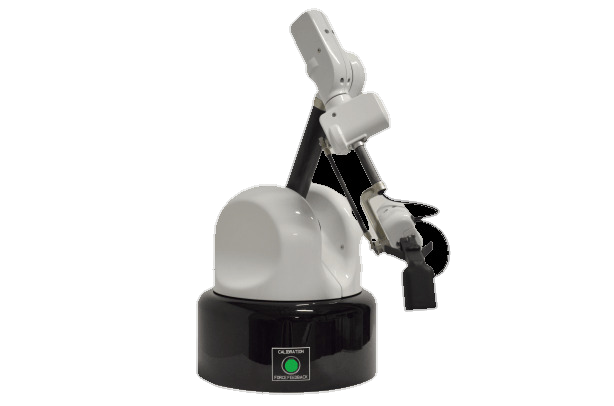
\includegraphics[width=22mm]{desktop-6D-compact-force-feedback-device-white.png}};
\node[lab, below=0mm of device] {Haptic device};
\draw[core] (0.95,14.6) -- node[right, lab]{$p_h, R_h$} (0.95,13.25);
\draw[core] (0.25,13.25) -- node[left, lab]{$w_h$} (0.25,14.6);

\node[blk=23mm] (fr)  at (4.4,13.3) {Force\\rendering};
\node[blk=23mm] (map) at (4.4,11.5) {Teleoperation\\mapping};
\begin{pgfonlayer}{background}
\node[grp, fit=(map)(fr), fill=black!3, draw=black!45] (tgrp) {};
\end{pgfonlayer}
\node[gtitle, black!60] at (tgrp.north) {Teleoperation};
\draw[core] (1.75,11.5) -- node[above, lab, align=center]{$p_h, R_h$\\$v_h,\omega_h$} (map.west);
\draw[core] (fr.west) -- node[above, lab]{$w_h$} (1.75,13.3);

% ---------------- shared autonomy ----------------
\node[blk] (intent) at (8.5,13.3) {Intent\\estimation};
\node[blk] (pol)    at (11.8,13.3) {Goal\\policies};
\node[blk] (arb)    at (10.15,11.5) {Arbitration};
\begin{pgfonlayer}{background}
\node[grp, fit=(intent)(pol)(arb), fill=orange!7, draw=orange!55!black] (sagrp) {};
\end{pgfonlayer}
\node[gtitle, orange!55!black] at (sagrp.north) {Shared autonomy};

\draw[core] (pol.west) -- node[above, lab]{$\pi_k^{\text{user}}$} (intent.east);
\draw[core] (map.east) -- node[below, lab, pos=0.3]{$v_{\text{user}}$} (arb.west);
\draw[core] (7.95,11.5) -- (7.95,12.9);
\draw[optB] (9.0,12.9) -- node[left, lab, pos=0.4]{$b_k$} (9.65,11.9);
\draw[optB] (11.3,12.9) -- node[right, lab, pos=0.4]{$\pi_k$} (10.65,11.9);
\node[tagl] at (10.15,12.65) {B};
\draw[optF] (intent.west) -- node[above, lab]{$b_k,\pi_k^{\text{user}}$} node[below=1pt, tagl]{F} (fr.east);

% ---------------- safety controller ----------------
\node[blk] (gov)   at (14.6,9.0) {Reference\\limiter};
\node[blk] (qp)    at (14.6,7.3) {\mbox{CLF--CBF QP}};
\node[blk] (col)   at (14.6,5.6) {Collision\\manager};
\node[blk] (sched) at (11.0,9.0) {Slack\\schedule};
\begin{pgfonlayer}{background}
\node[grp, fit=(gov)(qp)(col)(sched), fill=blue!6, draw=blue!45!black] (sfgrp) {};
\end{pgfonlayer}
\node[gtitle, blue!45!black] at (sfgrp.north) {Safety controller};

\draw[core] (arb.east) -- node[above, lab, pos=0.5]{$x_{\text{ref}}, \dot{x}_{\text{ref}}$} (14.6,11.5) -- (gov.north);
\draw[core] (gov) -- node[right, lab]{$x_g, v_g$} (qp);
\draw[core] (col) -- node[left, lab]{$J_{\text{soft}}, h_{\text{soft}}, d_{\text{safe}}$} (qp);
\draw[core] ($(qp.west)+(0,0.2)$) coordinate (qlam) -- node[above, lab, pos=0.4]{$\lambda_{\text{cbf}}, \lambda_{\text{jl}}$} (qlam -| {$(sched.south)+(-0.4,0)$}) -- ($(sched.south)+(-0.4,0)$);
\draw[core] ($(sched.south east)+(-0.2,0)$) -- node[above right, lab, inner sep=0.5pt, pos=0.55]{$w_{\delta}$} ($(qp.north west)+(0.3,0)$);

% ---------------- robot ----------------
\node (robot) at (5.2,6.9) {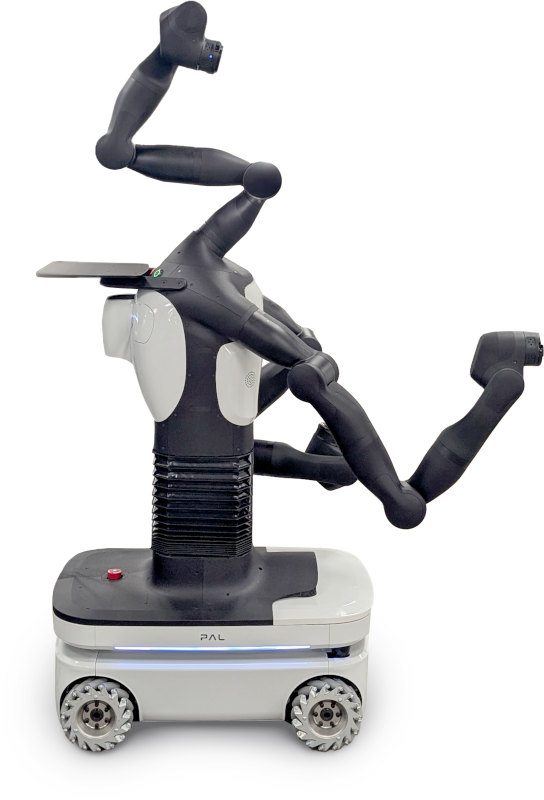
\includegraphics[width=20mm]{triago.png}};
\node[lab, left=0mm of robot] {TRIAGo};
\draw[core] ($(qp.west)+(0,-0.2)$) coordinate (qdot) -- node[below, lab, pos=0.9]{$\qdot^{\star}$} (qdot -| 6.2,0);
\draw[core] (col.west -| 6.2,0) -- node[below, lab, pos=0.25]{$q,\ \qdot^{\text{meas}}$} (col.west);

% ---------------- perception and world ----------------
\node[blk] (head)  at (5.2,2.6) {Head\\perception};
\node[blk] (perc)  at (9.0,2.6) {Perceived\\world};
\node[blk] (decl)  at (12.6,2.6) {Declared\\world};
\begin{pgfonlayer}{background}
\node[grp, fit=(head)(perc)(decl), fill=black!4, draw=black!45] (pwgrp) {};
\end{pgfonlayer}
\node[gtitle, black!60, anchor=north] at (pwgrp.south) {Perception and world};
\draw[core] (robot.south) -- node[right, lab]{RGB-D image} (head.north);
\draw[core] (head.east) -- node[above, lab]{$\hat{\mathcal{O}}$} (perc.west);
\coordinate (wsel) at (10.8,3.9);
\draw[selArr] (perc.north) |- (wsel);
\draw[selArr] (decl.north) |- (wsel);
\fill[black!60] (wsel) circle (0.6mm);
\draw[core] (wsel) -- (10.8,4.5) -- (18.1,4.5) -- node[right, lab, pos=0.5]{$\mathcal{G}$} (18.1,14.4) -- (11.8,14.4) -- (pol.north);
\draw[core] (14.6,4.5) -- node[right, lab]{$\mathcal{O}$} (col.south);
\draw[core] (col.east) -- (16.4,5.6) -- node[right, lab, pos=0.5]{$J_{\text{safe}}, b_{\text{safe}}$} (16.4,13.3) -- (pol.east);

\end{tikzpicture}}
\caption{System architecture. Ellipses and pictures are the human and physical endpoints, rounded rectangles are software nodes, grouped by layer. The operator sets the pose $(p_h, R_h)$ of the haptic device's handle, whose pose and twist $(v_h, \omega_h)$ the teleoperation mapping, clutch or joystick, turns into the commanded twist $v_{\text{user}}$; the operator feels the wrench $w_h$~\eqref{eq:wtotal}. Intent estimation scores $v_{\text{user}}$ against the per-goal policies $\pi_k^{\text{user}}$ into the belief $b_k$, and arbitration blends $v_{\text{user}}$ with the belief-weighted policies $\pi_k$~\eqref{eq:blend} into the reference pose $x_{\text{ref}}$ and its feed-forward twist $\dot{x}_{\text{ref}}$. The two assistance channels are orange: channel B (dashed) feeds $b_k$ and $\pi_k$ to arbitration, and without it $x_{\text{ref}}$ is the operator's own reference; channel F (dotted) feeds them to force rendering, which then adds the guidance force $w_{\text{guide}}$~\eqref{eq:fguide}. The reference limiter bounds $x_{\text{ref}}$ into $(x_g, v_g)$, the CLF--CBF QP returns the joint velocity $\qdot^{\star}$ under the barrier $(J_{\text{soft}}, h_{\text{soft}}, d_{\text{safe}})$, and its shadow prices $\lambda_{\text{cbf}}, \lambda_{\text{jl}}$ set the slack weight $w_\delta$~\eqref{eq:slacksched}. The collision manager builds the barrier from the measured state $(q, \qdot^{\text{meas}})$ and the obstacle set $\mathcal{O}$, and passes its Cartesian form $(J_{\text{safe}}, b_{\text{safe}})$ to the goal policies. Exactly one world source is active (grey dashed): the declared layout or the perceived world frozen from the head's estimate $\hat{\mathcal{O}}$; it also defines the goal set $\mathcal{G}$.}
\label{fig:arch}
\end{figure}

%───────────────────────────────────────────────────────────────────────────────
\section{Task setting and world model}
\label{sec:task}

The robot works at a fixed tabletop workcell. Rigid cylinders of known radius stand on the table; each must be picked up, transported, and set upright on a delivery station --- a conveyor infeed or an intermediate handover disk --- mounted on a unit beside the table. A cylinder admits two grasp families: a \emph{top grasp}, approaching along world $-Z$ with a free roll about the cylinder axis, and a \emph{side grasp}, approaching horizontally at a free azimuth and a free height along the body. Which family is usable in a layout is fixed by the overhead clearance --- a shelf or canopy over the table closes the top corridor and forces side grasps, an unobstructed ceiling admits top grasps. A layout may also place a delivery station within reach of only one arm, so that clearing the table requires the arms to hand a cylinder between them, or it may give each arm a station within its own reach; the two cases exercise, respectively, the coordinated and the independent behaviour of the bimanual controller. The concrete layouts used for evaluation are specified in the setup of the user study (Section~\ref{sec:study}).

Two representations of this scene coexist and are kept distinct. The \emph{visual} scene carries full industrial dressing --- fences, gantries, cabinets, the stations' own frames --- for the operator's spatial context only. The \emph{collision} world seen by the safety controller is a separate, deliberately small set of declared convex colliders: the table, each cylinder, the layout's blocking structure, and one convex envelope per station unit. The collision and joint-limit barrier constraints developed later in this chapter are stated over this declared model, so a fixture that is drawn but not declared lies outside them by construction. A cylinder is a world obstacle until grasped; on grasp it is attached to the gripper frame and carried with the arm as a moving collider, as the grasp lifecycle below details.

The shared-autonomy layer, developed later in this chapter, represents every admissible grasp and every admissible placement as a goal.

%───────────────────────────────────────────────────────────────────────────────
\section{QP-CLF-CBF safety controller}
\label{sec:qp}

\subsection{Decision variables and complete formulation}

Let $n_v$ be the velocity dimension of the full kinematic model~\cite{carpentier2019} and let $\mathcal{A}$ denote the index set of the 14 actuated arm joints (7 per arm; every other joint --- head, torso, base, grippers --- is locked, see below). The decision vector is
\begin{equation}
x \;=\; \bigl[\,\qdot,\;\; \delta_R,\;\; \delta_L\,\bigr] \in \mathbb{R}^{n_v+2},
\end{equation}
where $\qdot \in \mathbb{R}^{n_v}$ is the commanded joint velocity and $\delta_R,\delta_L \in \mathbb{R}$ are scalar tracking-relaxation (slack) variables, one per arm. At every control tick the controller solves a strictly convex QP, a safety filter that pairs a control Lyapunov function (CLF) for task tracking with a control barrier function (CBF) for collision avoidance, in the standard form of~\cite{ames2017cbf,ames2019ecc},
\begin{equation}
\label{eq:cost}
\min_{\qdot,\,\delta_R,\,\delta_L}\;
\underbrace{\sum_{i=1}^{n_v}\lambda_i\,\qdot_i^{2}}_{\text{damping}}
+ \underbrace{w_c\sum_{i\in\mathcal{A}}\bigl(\qdot_i - v_i^{\text{post}}\bigr)^2}_{\text{posture field}}
+ \underbrace{\sum_{X} w_{\delta,X}\,\delta_X^2}_{\text{CLF slack}}
+ \underbrace{\sum_{i\in\mathcal{A}} \rho_i\bigl(\qdot_i - \qdot_i^{\text{meas}}\bigr)^2}_{\text{rate damping}},
\end{equation}
subject to, for each arm $X \in \{R, L\}$,
\begin{align}
\hat{e}_{w,X}^{\top} J_{\text{task},X}\,\qdot \;+\; \delta_X \;&\ge\; \hat{e}_{w,X}^{\top}\dot{x}_{\text{ref},X} + \tfrac{\gamma_X}{2}\,\|e_{w,X}\|, && \text{(CLF)} \label{eq:clf}\\
J_{\text{soft},X}\,\qdot \;&\ge\; -\gamma_{\text{cbf}}\,\bigl(h_{\text{soft},X} - d_{\text{safe},X}\bigr), && \text{(CBF)} \label{eq:cbf}\\
\qdot_{\min,i}^{\text{safe}} \;\le\; \qdot_i \;&\le\; \qdot_{\max,i}^{\text{safe}} \quad \forall i. && \text{(joint limits)} \label{eq:jl}
\end{align}
Here:
\begin{itemize}[nosep]
\item $\lambda_i$ is the $i$-th component of the per-joint damping weight vector, $\lambda_i = \lambda$ for every joint from a single scalar base damping $\lambda > 0$, raised on a frozen arm's joints, as detailed in the bimanual-coupling discussion below. (Throughout, bare $\lambda$ denotes this damping scalar; Lagrange multipliers are always subscripted, e.g.,\ $\lambda_{\text{cbf}}$, $\lambda_{\text{jl}}$ --- introduced with the adaptive scheduling law below);
\item $v^{\text{post}}$ is the posture-field reference velocity and $w_c$ its scalar weight, defined with the posture task below, nonzero only on $\mathcal{A}$;
\item $w_{\delta,X}$ is the adaptively scheduled slack weight of arm $X$, defined with the scheduling law below;
\item $\rho_i$ is the per-arm \emph{scheduled} rate-damping weight and $\qdot^{\text{meas}}$ the \emph{measured} joint velocity, both defined with the rate-damping term below; the term exists only on $\mathcal{A}$;
\item $e_{w,X} = W_{\text{task}}\,e_X$ is the diagonally weighted task error of arm $X$, $\hat{e}_{w,X}$ its unit vector, $J_{\text{task},X}$ the arm's 6D frame Jacobian, $\dot{x}_{\text{ref},X}$ the reference feed-forward twist, and $\gamma_X$ the arm's CLF convergence rate;
\item $h_{\text{soft},X}$ is arm $X$'s collision barrier, a smooth lower approximation (SoftMin) of the smallest distance between that arm and anything it may collide with, and $J_{\text{soft},X}$ its gradient, the row that maps joint velocities into the rate of change of that clearance, $\dot{h}_{\text{soft},X} = J_{\text{soft},X}\,\qdot$, both constructed in Section~\ref{sec:cbf}; $d_{\text{safe},X}$ its velocity-dependent safety margin, $\gamma_{\text{cbf}}$ the class-$\mathcal{K}$ barrier gain.
\end{itemize}
Joints outside $\mathcal{A}$ are hard-locked to zero velocity by two opposing rows of~\eqref{eq:jl} ($0 \le \qdot_i \le 0$), rendering the head, torso, base, and grippers kinematically frozen from the QP's perspective. Every cost term leaves a zero gradient on those locked joints, a requirement for feasibility that the rate-damping term below must also respect.

The QP is solved with a dual active-set method (Goldfarb--Idnani~\cite{goldfarb1983}, \texttt{quadprog}). On the rare infeasible tick the commanded velocity is zeroed for that tick, a zeroed setpoint whose consequences are discussed among the limitations (Section~\ref{sec:concllimitations}).

\subsection{CLF --- task tracking with relaxation}
\label{sec:clf}

For each arm, the task error is $e_X = x_{\text{ref},X} - x_X$ --- stacked position error and orientation error ($\log_3$ of the relative rotation). Let $W_{\text{task}}$ be the diagonal, strongly position-dominant task-weight matrix, $e_{w,X} = W_{\text{task}}\,e_X$ the weighted error, and $\hat{e}_{w,X} = e_{w,X}/\|e_{w,X}\|$ its unit direction (for $e_{w,X} \neq 0$); the position dominance of $W_{\text{task}}$ is what makes orientation yield first when tracking and safety conflict.

Row~\eqref{eq:clf} is the normalised decrease condition of the quadratic candidate
\begin{equation}
V_X^{q} = \tfrac{1}{2}\,e_X^{\top} W_{\text{task}}\,e_X,
\qquad
\nabla_{e_X} V_X^{q} = W_{\text{task}}\,e_X = e_{w,X},
\label{eq:clfquadgrad}
\end{equation}
so $\hat{e}_{w,X}$ is exactly the unit gradient of $V_X^{q}$, with no factor of $W_{\text{task}}$ left over. With $\dot{e}_X = \dot{x}_{\text{ref},X} - J_{\text{task},X}\,\qdot$, imposing the normalised decrease $\hat{e}_{w,X}^{\top}\dot{e}_X \le -\tfrac{\gamma_X}{2}\,\|e_{w,X}\| + \delta_X$ with slack $\delta_X \ge 0$ and rearranging returns~\eqref{eq:clf} exactly. This inequality is \emph{not} the derivative of $\|e_{w,X}\|$ itself, which would carry an extra factor of $W_{\text{task}}$; scaling it instead by $\|e_{w,X}\| \ge 0$ gives the exact rate of $V_X^{q}$,
\begin{equation}
\dot{V}_X^{q} = e_{w,X}^{\top}\dot{e}_X = \|e_{w,X}\|\,\hat{e}_{w,X}^{\top}\dot{e}_X \;\le\; -\tfrac{\gamma_X}{2}\,\|e_{w,X}\|^2 + \delta_X\|e_{w,X}\|,
\label{eq:clfnorm}
\end{equation}
where the inequality is the imposed row. Writing $w_{\min}$ and $w_{\max}$ for the smallest and largest diagonal entries of $W_{\text{task}}$, $\|e_{w,X}\|^2 = e_X^{\top}W_{\text{task}}^2 e_X \ge w_{\min}\,e_X^{\top}W_{\text{task}}e_X = 2w_{\min}V_X^{q}$, so~\eqref{eq:clfnorm} certifies
\begin{equation}
\dot{V}_X \;\le\; -\tfrac{\gamma_X w_{\min}}{2}\,V_X + \sqrt{w_{\max}}\,\delta_X, \qquad V_X = \sqrt{2V_X^{q}} = \bigl(e_X^{\top}W_{\text{task}}e_X\bigr)^{1/2},
\label{eq:clfrate}
\end{equation}
for the weighted-norm candidate $V_X$ --- positive definite, radially unbounded, continuously differentiable away from $e_X = 0$, admissible if non-smooth at the origin (Section~\ref{sec:sota-clf-cbf-qp}) --- a valid relaxed exponential decrease, but at rate $\gamma_X w_{\min}/2$, not the naive $\gamma_X/2$. Under a position-dominant $W_{\text{task}}$, $w_{\min}$ is an orientation weight, so the certified rate is lowest for a purely rotational error and larger for a positional one; raising the orientation weights, as the grasp phase does, raises $w_{\min}$ and with it the worst-case rate. The normalisation is therefore a genuine trade of certified rate for conditioning, not a free simplification: $\hat{e}_{w,X}^{\top}J_{\text{task},X}$ is positively homogeneous of degree zero in $e_X$ (unit norm at every error magnitude) rather than degree one, so it neither grows unbounded far from the target nor vanishes at it. Positivity of $\delta_X$ is implicit --- it enters no other constraint and is quadratically penalised, so the optimum never drives it below what the row requires; through the same scaling, $\delta_X$ enters the certified decrease not as a bare offset but rescaled by $\|e_{w,X}\|$, and hence by at most $\sqrt{w_{\max}}$ in~\eqref{eq:clfrate}.

The decrease condition of $V_X^{q}$ itself,
\begin{equation}
(W_{\text{task}}e_X)^{\top} J_{\text{task},X}\,\qdot + \delta_X
\;\ge\;
(W_{\text{task}}e_X)^{\top}\dot{x}_{\text{ref},X} + \gamma_X\, V_X^{q}
\label{eq:clfquad}
\end{equation}
has a row vector $W_{\text{task}}e_X$ and a closing-speed demand $\gamma_X V_X^{q}$ that both grow with $e_X$ --- near-singular rows far from the reference, vanishing tracking authority close to it. Row~\eqref{eq:clf} is exactly~\eqref{eq:clfquad} divided by $\|\nabla_{e_X} V_X^{q}\| = \|e_{w,X}\|$: the same descent direction $\hat{e}_{w,X}$, but a unit-norm coefficient instead of one that blows up far from the target and disappears at it, at the price of the reduced certified rate in~\eqref{eq:clfrate}.

The slack is the single most important design element for feasibility: because $\delta_X$ appears only in arm $X$'s CLF row and in the cost, the CLF can \emph{always} yield to the hard constraints \eqref{eq:cbf}--\eqref{eq:jl}. Tracking degrades gracefully under conflict; safety never does.

The rate $\dot{e}_X$ above treats the orientation channel as the plain angular-velocity difference $\omega_{\text{ref},X} - \omega_X$, a first-order approximation of the true $SO(3)$ kinematics of the orientation error that is exact only as the error vanishes. The approximation is left uncorrected because the reference limiter keeps that error small and $W_{\text{task}}$'s low orientation weight further discounts whatever residual it leaves in~\eqref{eq:clf}.

\subsection{CBF --- per-arm SoftMin collision barrier}
\label{sec:cbf}

Collision avoidance is enforced over a capsule-based geometric model of both arms (dominant-axis-snapped capsules per link, box-approximated grippers, body/ground/wall colliders). The declared pairs cover each arm against the world obstacles, each arm against the other, each arm against itself (its distal hand against its own proximal links), and each arm against the head chain, whose live forward-kinematic capsules enter as a quasi-static obstacle with no head joint in the QP decision vector. Each tick, all declared pairs are queried for signed distance $d_k(q)$; pairs within a filter radius are sorted and the $K$ closest retained.

A single minimum-distance constraint is non-smooth, so the barrier aggregates the active set through a SoftMin --- a log-sum-exp composition in the spirit of nonsmooth barrier composition~\cite{glotfelter2017}. The key architectural decision is a \emph{per-arm decomposition}: two independent barriers are assembled, where $\mathcal{P}(X)$ is the subset of active pairs touching at least one geometry belonging to arm $X$ (its own links and gripper, or a cylinder it currently holds):
\begin{align}
h_{\text{soft},X}(q) &= -\frac{1}{\alpha_s}\,\log\!\!\sum_{k \in \mathcal{P}(X)} e^{-\alpha_s d_k(q)}, \notag\\[2pt]
J_{\text{soft},X}(q) &= \sum_{k \in \mathcal{P}(X)} \sigma_k\, J_k(q),
\qquad
\sigma_k = \frac{e^{-\alpha_s d_k}}{\sum_{j \in \mathcal{P}(X)} e^{-\alpha_s d_j}},
\label{eq:softmin}
\end{align}
where $\alpha_s$ is the aggregation sharpness, $J_k$ is pair $k$'s distance Jacobian (witness-point Jacobian difference projected on the witness normal), and $\sigma_k$ are softmax weights. $h_{\text{soft},X}$ is a smooth lower approximation of the true minimum distance restricted to arm $X$'s pairs, and $J_{\text{soft},X}$ is the convex blend of exactly those pairs' Jacobians --- hence it has zero columns in the \emph{other} arm's joints unless a pair genuinely involves both arms. A genuine inter-arm pair contributes to both $\mathcal{P}(R)$ and $\mathcal{P}(L)$, preserving the ability of either arm to yield for the other.

Without the split, a single SoftMin row would mix all pairs and let the QP recruit the idle arm's joints to cheaply satisfy a barrier activated solely by the active arm near an unrelated obstacle, producing spurious idle-arm motion and oscillation. The same coupling concern applies to the safety margin, which is therefore also split per arm and made velocity-dependent, so that a faster-moving arm is held back sooner,
\begin{equation}
d_{\text{safe},X} \;=\; d_0 + k_v\,\|\qdot_X\|,
\label{eq:dsafe}
\end{equation}
computed from each arm's \emph{own} 7-joint velocity vector $\qdot_X$, with base margin $d_0$ and gain $k_v$.

\textbf{$d_{\text{safe},X}$ as a Cartesian closing-speed bound.} Consider a pair $k \in \mathcal{P}(X)$ that touches only arm $X$'s own geometry, that is, its links, its gripper, or an object it currently holds, re-parented onto the wrist joint at grasp. Writing $J_k = n_k^{\top}(J_{p_1} - J_{p_2})$, with $n_k$ the unit witness normal and $J_{p_1}$, $J_{p_2}$ the translational Jacobians of the two witness points, $J_k$ has nonzero entries only on arm $X$'s columns for such a pair, so the signed distance's time derivative is $\dot{d}_k = J_k(q)\,\qdot_X$. Each column $i$ of a revolute joint's point Jacobian equals $z_i \times (p - o_i)$, with $z_i$ the unit axis of joint $i$ and $o_i$ a point on it, a vector whose norm is the perpendicular distance from axis $i$ to the point $p$. Bounding every such lever arm on arm $X$, and on any object it holds, by $r_{\max}$, and applying the Cauchy--Schwarz inequality over the $n_A = 7$ columns of arm $X$, gives
\begin{equation}
\|J_k\|_2 \;\le\; \ell_{\max} \;=\;
\begin{cases}
\sqrt{n_A}\,r_{\max}, & \text{world pair } (J_{p_2} = 0),\\[2pt]
2\sqrt{n_A}\,r_{\max}, & \text{self-collision pair,}\\
 & \text{both witness points on arm } X,
\end{cases}
\label{eq:lmax}
\end{equation}
the self-collision bound being loose because the shared proximal columns of $J_{p_1}$ and $J_{p_2}$ partially cancel. A second use of the Cauchy--Schwarz inequality, on $\dot{d}_k = J_k\,\qdot_X$, gives $|\dot{d}_k| \le \|J_k\|_2\,\|\qdot_X\| \le \ell_{\max}\,\|\qdot_X\|$, so that
\begin{equation}
\begin{split}
d_{\text{safe},X} &\;=\; d_0 + k_v\,\|\qdot_X\| \;\ge\; d_0 + \tau_v\,|\dot{d}_k|, \\
\tau_v &\;\triangleq\; \frac{k_v}{\ell_{\max}},
\end{split}
\label{eq:tauv}
\end{equation}
for every such pair, where only the closing, rather than separating, sense of $\dot{d}_k$ matters, since the barrier only restrains approach. Equation~\eqref{eq:dsafe} is therefore a conservative over-approximation of a Cartesian approach-speed margin with time horizon $\tau_v$, which also shows that $k_v$ carries units of length$\times$time/angle rather than time alone (Appendix~\ref{app:config}). Taking $r_{\max}$ as the arm's own shoulder-to-fingertip reach fixes $\ell_{\max}$, and with it the time horizon $\tau_v$ that Equation~\eqref{eq:dsafe}'s $k_v$ actually realises (Appendix~\ref{app:config}). Two cases remain uncovered by this bound: an inter-arm pair, whose true closing speed also depends on the other arm's $\qdot$ and is captured only by an optional inter-arm closing-margin term, disabled in every reported trial, and a head-vs-arm pair, whose margin on the arm side structurally cannot see the head's own motion, a coupling taken up in the bimanual-coupling discussion below. Only the current-tick value of $d_{\text{safe},X}$ enters the enforced row~\eqref{eq:cbf}; its own time derivative, $k_v\,\frac{d}{dt}\|\qdot_X\|$, is not enforced, since the QP is a velocity-level program with no $\ddot{q}$ decision variable to carry it.

Constraint~\eqref{eq:cbf} then enforces the class-$\mathcal{K}$ barrier condition $\dot{h} \ge -\gamma_{\text{cbf}}\,(h - d_{\text{safe}})$ on each arm's aggregate: the arm may approach an obstacle only at a rate that vanishes as the margin approaches $d_{\text{safe},X}$, enforcing, on each arm's aggregate, a nominal barrier condition on the sampled state rather than a certified physical invariance (Section~\ref{sec:concllimitations}); the SoftMin approximation itself errs on the conservative side.

The aggregation sharpness $\alpha_s$ is set to a high value, for a reason that becomes acute in cluttered geometry. The log-sum-exp in~\eqref{eq:softmin} under-approximates the true minimum distance over $\mathcal{P}(X)$ by at most $\alpha_s^{-1}\ln|\mathcal{P}(X)|$, so a larger $\alpha_s$ both tightens $h_{\text{soft},X}$ onto $\min_k d_k$ and concentrates the softmax weights $\sigma_k$ onto the genuinely nearest pair. When an arm is boxed in --- a table below, a shelf above, structural legs alongside --- many pairs sit at nearly equal distance while their witness normals point in genuinely different directions. A low $\alpha_s$ then averages those directions in $J_{\text{soft},X}$ toward mutual cancellation, shrinking $\|J_{\text{soft},X}\|$ with no real loss of clearance; through~\eqref{eq:cbf} this drives up the collision shadow price $\lambda_{\text{cbf},X}$, the quantity the adaptive scheduling law below tracks --- which varies roughly as $\|J_{\text{soft},X}\|^{-2}$ --- and inflates the apparent cost of a clearance deficit that is not physically present. A sharp $\alpha_s$ keeps the blend~\eqref{eq:softmin} dominated by the single closest pair, so $J_{\text{soft},X}$ retains the magnitude and direction of a true nearest-obstacle gradient.

\subsection{Posture task --- gradient potential field}
\label{sec:posture}

Redundancy not consumed by the tracking row is shaped by a posture field: the negative gradient of a scalar joint-limit potential, folded into the QP cost~\eqref{eq:cost} rather than projected through the null space, so the solver arbitrates it against tracking and the hard rows instead of subordinating it to them. The potential is an inverse-square repulsive barrier --- the joint-limit counterpart of the gradient-projection criteria of Li\'egeois~\cite{liegeois1977} and of Zghal, Dubey, and Euler~\cite{zghal1990} --- with one term per bound and the distance-to-limit in place of a distance-to-obstacle. It is evaluated on the \emph{normalised} joint coordinate, so every joint is defended at the same fraction of its travel toward whichever bound it approaches. For joint $i$ with limits $[q_i^{\ell}, q_i^{u}]$, midpoint $\bar{q}_i$, and half-range $\Delta_i = \tfrac{1}{2}(q_i^{u} - q_i^{\ell})$:
\begin{align}
p_i &= \operatorname{clip}\!\Bigl(\frac{q_i - \bar{q}_i}{\Delta_i},\, -1+\varepsilon,\, 1-\varepsilon\Bigr),
&
H(p) &= \frac{1}{(1-p)^2} + \frac{1}{(1+p)^2},
\\
\frac{dH}{dp} &= \frac{2}{(1-p)^3} - \frac{2}{(1+p)^3},
&
v_i^{\text{post}} &= \operatorname{clip}\!\Bigl(-k_g\,\frac{dH}{dp}\Big|_{p_i},\; \pm v_{\max}^{\text{post}}\Bigr),
\end{align}
where $k_g$ is the gradient gain, $v_{\max}^{\text{post}}$ a hard clamp for solver safety, and the interior clamp $\varepsilon$ keeps the gradient finite and correctly signed even at or beyond a limit --- the raw cube would flip sign there and drive the joint \emph{out}. At the midpoint $p_i = 0$, so $dH/dp = 0$ and $v_i^{\text{post}}$ vanishes; toward either bound $|p_i| \to 1$ and $H$ diverges. The field is therefore negligible through mid-range --- leaving full redundancy to the CLF --- and grows sharply only near a limit. During autonomous precision phases the posture weight $w_c$ is smoothly ramped to a small fraction of its nominal value by a first-order filter, so the QP spends the redundancy on tracking rather than centring.

\subsection{Rate damping --- measured-velocity anchor}
\label{sec:rate}

The rate term in~\eqref{eq:cost} penalises deviation from the \emph{measured} joint velocity $\qdot^{\text{meas}}$ on the active joints $\mathcal{A}$. Under a position-dominant $W_{\text{task}}$ the wrist directions are task-null for~\eqref{eq:clf} and are resolved by the cost alone, which without this term carries no memory of the previous tick; the anchor supplies that memory from the arm's physical state. The weight $\rho_i$ trades tracking against damping and is scheduled per arm between two values (Appendix~\ref{app:config}), full only near convergence: at large error a strong pull toward a near-zero measured velocity re-suppresses every departing command and stalls the arm. Two properties are structural. The anchor is the measured velocity, not the controller's own previous output $\qdot^{\star}_{k-1}$, which would instead close a self-referential loop, pulling the command toward its own history rather than the arm's state. The restriction to $\mathcal{A}$ is likewise required for feasibility: joints outside $\mathcal{A}$ are already pinned by~\eqref{eq:jl}, and an unmasked term would contest that pin. Empirically, the term proves necessary on the physical robot: left unanchored, exactly these task-null directions develop a persistent high-frequency oscillation in the commanded velocity, damped by anchoring the cost to the arm's actual state.

\subsection{Adaptive scheduling via KKT shadow prices}
\label{sec:sched}

Every solve of~\eqref{eq:cost} returns, together with the command, the Karush--Kuhn--Tucker (KKT) Lagrange multipliers of its constraints. At the optimum, the multiplier of an active row is its \emph{shadow price}: the rate at which the optimal cost would decrease if that row were relaxed by one unit~\cite{boyd2004}. It is zero while the row is inactive and grows with how much of the task the row is holding back. The multipliers of the safety rows therefore carry, at no additional computational or sensing cost, a quantitative measure of how difficult the current situation is for the controller: an arm moving through free space has null prices, while an arm whose reference drives it into a table or toward a joint stop has large ones. This section exploits that signal so that the robot assesses the difficulty of its own surroundings from its own optimisation and adapts its behaviour to it, with no separate environment classifier, no distance threshold, and no operator input. One rule governs every adaptation: when the surroundings are easy, the task is executed at full precision and full speed; when they become hard, precision and timing are relaxed first, so that the one requirement that is never relaxed, safety, keeps its full authority.

\textbf{Why a fixed tracking priority is inadequate.} The slack weight $w_{\delta,X}$ is the price of tracking error in~\eqref{eq:cost}, and a single fixed value has to serve two regimes with opposite needs. Drop the arm index and retain, for one arm, only the quadratic velocity terms of the cost, with diagonal Hessian $D \succ 0$, the CLF row~\eqref{eq:clf} written as $a^{\top}\qdot + \delta \ge c$, with $a = J_{\text{task}}^{\top}\hat{e}_w$, and the CBF row~\eqref{eq:cbf} as $n^{\top}\qdot \ge b$, with $n = J_{\text{soft}}^{\top}$. Stationarity of the Lagrangian gives
\begin{equation}
2D\qdot = \lambda_{\text{clf}}\,a + \lambda_{\text{cbf}}\,n,
\qquad
2w_{\delta}\,\delta = \lambda_{\text{clf}},
\label{eq:kktstat}
\end{equation}
with $\lambda_{\text{clf}}, \lambda_{\text{cbf}} \ge 0$ the multipliers of the two rows. In free space only the CLF row is active, $\lambda_{\text{cbf}} = 0$, and~\eqref{eq:kktstat} yields the residual slack
\begin{equation}
\delta^{\star} = \frac{c}{1 + w_{\delta}\,a^{\top}D^{-1}a},
\label{eq:freeslack}
\end{equation}
which decreases as $1/w_{\delta}$: free-space precision asks for a \emph{high} weight. When the reference instead drives the arm into the barrier, both rows are active. Writing $A = a^{\top}D^{-1}a$, $N = n^{\top}D^{-1}n$, and $C = a^{\top}D^{-1}n < 0$ (the tracking direction points into the obstacle), solving~\eqref{eq:kktstat} with both rows tight gives
\begin{equation}
\lambda_{\text{clf}} = \frac{2\,(c - bC/N)}{A_{\perp} + 1/w_{\delta}},
\qquad
\lambda_{\text{cbf}} = \frac{2b + \lambda_{\text{clf}}\,\lvert C\rvert}{N},
\qquad
A_{\perp} = A - \frac{C^2}{N} \ge 0,
\label{eq:kktconflict}
\end{equation}
where $A_{\perp}$ measures the tracking authority left in directions that do not touch the barrier. When the reference points squarely into the obstacle, $A_{\perp} \ll 1/w_{\delta}$ and both multipliers grow linearly with $w_{\delta}$. A high weight then buys no tracking --- the obstructed part of the demand cannot be met at any price --- and only inflates the multipliers, with two consequences on the sampled loop.

First, by~\eqref{eq:kktstat} the barrier contributes the term $\tfrac{1}{2}D^{-1}n\,\lambda_{\text{cbf}}$ to the command. When the row leaves the active set --- the arm slides past the obstacle, a pair leaves the activation radius, or the SoftMin switches its dominant pair --- this term vanishes within one tick, so the step in $\qdot$ scales with $\lambda_{\text{cbf}}$: a stiff tracking weight turns every active-set change into an abrupt brake or a velocity oscillation rather than a smooth yield. Second, the slack guarantees feasibility of the CLF row by construction, but the hard rows must also be jointly feasible, and on the sampled loop this depends on the state. At tick $k+1$ the CBF row and the box~\eqref{eq:jl} admit a solution if and only if
\begin{equation}
\gamma_{\text{cbf}}\,\bigl(d_{\text{safe},k+1} - h_{\text{soft},k+1}\bigr) \;\le\; \max_{\qdot^{\text{safe}}_{\min} \le \qdot \le \qdot^{\text{safe}}_{\max}} J_{\text{soft}}\,\qdot,
\label{eq:hardfeas}
\end{equation}
the right-hand side being the recovery capacity of the box, which shrinks near a joint limit. In continuous time the barrier condition keeps the left-hand side non-positive. On the sampled loop, with the CBF row active at tick $k$, $h_{\text{soft},k+1} - d_{\text{safe},k+1}$ departs from its nominal value $(1 - \gamma_{\text{cbf}}\Delta t)(h_{\text{soft},k} - d_{\text{safe},k})$ by the second-order remainder of $h_{\text{soft}}$ over one tick, $O(\Delta t^2\|\qdot_k\|^2)$, by the growth $k_v\,\Delta\|\qdot\|$ of the margin~\eqref{eq:dsafe}, and by terms the nominal condition does not model (actuator lag, stale inputs, pair-set changes; Section~\ref{sec:concllimitations}), all of which grow with how hard the previous command pressed along the barrier. That command is, by~\eqref{eq:kktstat}, the one a large $\lambda_{\text{clf}}$ buys. Condition~\eqref{eq:hardfeas} therefore holds by design in the nominal model yet is violated in practice by commands that are too aggressive at the barrier: this is the mechanism by which the tracking weight, absent from every hard row, still decides whether the physical loop runs into infeasible ticks.

\textbf{Shadow-price filtering and slack schedule.} Raw multipliers are noisy from tick to tick, since active-set changes are discrete events, so every scheduled quantity is driven through a first-order low-pass filter (LPF), the exact zero-order-hold discretisation of $\tau\dot{y} = u - y$ at the control period $\Delta t$,
\begin{equation}
y_k = \text{LPF}_{\tau}(u)_k \;\triangleq\; e^{-\Delta t/\tau}\,y_{k-1} + \bigl(1 - e^{-\Delta t/\tau}\bigr)\,u_k,
\label{eq:lpf}
\end{equation}
with unit static gain and time constant $\tau$. After each solve, the multipliers of the two CBF rows ($\lambda_{\text{cbf},R}$, $\lambda_{\text{cbf},L}$) and of the joint-limit rows ($\lambda_{\text{jl}}$, reduced to a per-arm maximum) are filtered as $\bar{\lambda}_{(\cdot)} = \text{LPF}_{\tau_{\lambda}}(\lambda_{(\cdot)})$. The slack weight of arm $X$ is scheduled from its own driver $\bar{\lambda}_X = \max\bigl(\bar{\lambda}_{\text{cbf},X},\, \bar{\lambda}_{\text{jl},X}\bigr)$ through a quadratic-tolerance law followed by a second, independent LPF on its output:
\begin{equation}
w_{\delta,X}^{\text{tgt}} \;=\; w_{\delta}^{\text{base}} + e^{-\beta\,\bar{\lambda}_X^2}\,\bigl(w_{\delta}^{\max} - w_{\delta}^{\text{base}}\bigr),
\qquad w_{\delta,X} = \text{LPF}_{\tau_{w}}\bigl(w_{\delta,X}^{\text{tgt}}\bigr),
\label{eq:slacksched}
\end{equation}
each arm carrying its own filter states. In free space ($\bar{\lambda}_X \to 0$) the weight rises to its ceiling $w_{\delta}^{\max}$, which tightens tracking through~\eqref{eq:freeslack}; near an active constraint it falls to its floor $w_{\delta}^{\text{base}}$, which caps the multipliers of~\eqref{eq:kktconflict} --- independently of the other arm. The quadratic exponent keeps the law flat for small prices, so the chatter of a barely active row leaves free-space tracking untouched. The output stage is required because a shadow price observed on hardware to spike by orders of magnitude crosses the whole knee of the law within a fraction of $\tau_{\lambda}$, so the input filter alone still lets through a sharp one-tick weight change. The schedule closes a loop --- a higher weight presses the QP harder against the barrier, raising $\bar{\lambda}_X$, which the law returns as a lower weight --- whose stability is observed on hardware, not formally proven.

\textbf{Choice of the schedule range.} The two bounds are tuned in sequence, each against the regime it serves. The floor $w_{\delta}^{\text{base}}$ is fixed first, on the critical case: an arm close to an obstacle with a large tracking error. It is the largest weight for which that case produces neither infeasible ticks through~\eqref{eq:hardfeas} nor chattering through the active-set steps above. Because the schedule returns to $w_{\delta}^{\text{base}}$ whenever a constraint is strongly active, this tuning carries over to every configuration in which the conflict actually arises. The floor alone, however, leaves an imprecise free-space motion, by~\eqref{eq:freeslack}, so the ceiling $w_{\delta}^{\max}$ is then raised above it until free-space tracking is precise and still stable, with $\beta$ placing the knee between the two regimes. A single fixed weight must trade these two requirements against each other; the schedule separates them, at the cost of one exponential and two scalar filters per arm per tick.

\textbf{Scope of the contribution.} The contribution of this section is the use of the safety filter's own shadow prices as a self-assessment of how constrained the robot currently is, and the slack-weight schedule~\eqref{eq:slacksched} is its main instance, the one active and plotted in the trials of Chapter~\ref{ch:exp}. The same signal was exploited to regulate further behaviours, which support the same principle without being part of the reported evaluation. For an assigned trajectory with no operator in the loop, the reference is re-timed by a virtual clock $\vartheta$ whose rate $\nu$ drops as the worst collision price rises,
\begin{equation}
\begin{split}
\nu^{\text{tgt}} &= \nu_{\min} + (1 - \nu_{\min})\,e^{-k_{\nu}\max_X \lambda_{\text{cbf},X}},
\qquad
\nu = \text{LPF}_{\tau_{\nu}}\bigl(\nu^{\text{tgt}}\bigr),\\
\dot{\vartheta} &= \nu,
\qquad
x_{\text{ref}} = p(\vartheta),
\qquad
\dot{x}_{\text{ref}} = \nu\,\frac{\partial p}{\partial \vartheta}(\vartheta),
\end{split}
\label{eq:timescale}
\end{equation}
where $p(\vartheta)$ is the time-parametrised reference path, $\nu_{\min} \in (0,1)$ keeps the clock from stalling, and $k_{\nu}$ sets the sensitivity. The path geometry is unchanged; only its timing stretches near an obstacle, so the reference no longer runs ahead of an arm the barrier is holding back and the reference limiter of Section~\ref{sec:governor} is not left to clip it. This time scaling was tested on autonomous trajectory runs during development, where it slowed the motion near obstacles and ran stably; those runs are not reported with figures in this work. Along the same lines, the CLF rate $\gamma_X$ was scheduled over an interval $[\gamma_{\min}, \gamma_{\max}]$ by the same kernel as~\eqref{eq:slacksched}, and a per-joint posture weight by each joint's own joint-limit price; both are included here as directions opened by the same signal. Across these mechanisms the price of adaptation is low: in free space the robot tracks with full precision and at nominal speed, and once the scene becomes hard it gives up precision and execution time to preserve safety. Keeping a stiff tracking weight or a fixed schedule there would not complete an obstructed motion any faster, by~\eqref{eq:kktconflict}; it would only turn the conflict into multiplier spikes, abrupt brakes, and oscillation.

\subsection{Joint limits --- per-joint position-limit barrier}
\label{sec:jl}

Each actuated joint must stay inside its mechanical range, so the set to render forward-invariant is the joint-space box
\begin{equation}
\mathcal{C}_q \;=\; \bigl\{\, q \;:\; q_i^{\ell} \le q_i \le q_i^{u}\ \ \forall i \,\bigr\},
\label{eq:jlset}
\end{equation}
the intersection of the per-joint slabs $\mathcal{C}_i = \{\,q : q_i^{\ell} \le q_i \le q_i^{u}\,\}$. The arms are commanded at the velocity level, so each joint is a single integrator $\dot{q}_i = \qdot_i$ with $\qdot_i$ a decision variable, and forward invariance of $\mathcal{C}_q$ is secured by one linear barrier per bound. Let $d_i^{+} = q_i^{u} - q_i$ and $d_i^{-} = q_i - q_i^{\ell}$ be the distances to the upper and lower limit; each is $C^1$ and positive on the interior of its slab. With a speed-dependent buffer $b_i = b_0 + k_b\,\lvert\qdot_i^{\text{meas}}\rvert$ --- base margin $b_0 > 0$ and horizon gain $k_b > 0$ acting on the measured joint speed $\lvert\qdot_i^{\text{meas}}\rvert$ --- the barrier guarding the upper bound is $h_i^{+} = d_i^{+} - b_i$ and the one guarding the lower bound is $h_i^{-} = d_i^{-} - b_i$, each positive while the joint sits more than $b_i$ from that limit. Imposing the class-$\mathcal{K}$ barrier condition $\dot{h}_i^{+} \ge -k_p\,h_i^{+}$ with linear gain $k_p > 0$ and substituting the single-integrator kinematics $\dot{d}_i^{+} = -\qdot_i$, with $b_i$ held constant over one tick so that $\dot{h}_i^{+} \approx \dot{d}_i^{+}$, reduces the condition to a plain upper bound on the joint velocity, $\qdot_i \le k_p\,(d_i^{+} - b_i)$. The lower bound follows the same way from $h_i^{-}$, where $\dot{d}_i^{-} = \qdot_i$ gives $\qdot_i \ge -k_p\,(d_i^{-} - b_i)$. Combined with the model's hard velocity limit $\bar{v}_i$, these are the box~\eqref{eq:jl} bounds
\begin{equation}
\qdot_{\max,i}^{\text{safe}} = \min\!\bigl(\bar{v}_i,\; k_p(d_i^{+} - b_i)\bigr),
\qquad
\qdot_{\min,i}^{\text{safe}} = -\min\!\bigl(\bar{v}_i,\; k_p(d_i^{-} - b_i)\bigr).
\label{eq:jlbrake}
\end{equation}
Invariance follows from Nagumo's theorem~\cite{blanchini1999,ames2019ecc}: on the face $q_i = q_i^{u}$ the admissible interval collapses to $\qdot_i \le -k_p b_i < 0$, so any $\qdot$ satisfying the row points strictly into $\mathcal{C}_q$, and likewise on the lower face. The barrier is linear and one per bound, so the joint limits enter the QP as a hard box with no aggregation and no relaxation, unlike the collision barrier of Section~\ref{sec:cbf}. The buffer keeps the trajectory a margin $b_i$ inside the mechanical stop, and its growth with $\lvert\qdot_i^{\text{meas}}\rvert$ offsets the one-tick sampling lag, so the inward-pointing property survives discretisation and a fast joint begins braking earlier.

Unlike the collision barrier, the joint-limit barrier also holds in discrete time: the exact one-tick zero-order-hold condition $\qdot_i \le (q_i^u - q_i)/\Delta t$ is implied by the enforced bound $\qdot_i \le k_p(d_i^+ - b_i)$ whenever the gain $k_p$ is small relative to the tick rate $1/\Delta t$ (Appendix~\ref{app:config}), so~\eqref{eq:jlbrake} is discretely forward-invariant given faithful velocity tracking, without further assumption.

\subsection{Reference limiter}
\label{sec:governor}

An intermediate layer between the raw Cartesian reference and the CLF --- a reference limiter, inspired by but distinct from the reference-governor family~\cite{garone2017} --- bounds the speed, the acceleration, the position error, and the orientation error of the target the CLF is asked to track, so that a discontinuous, aggressive, or far-away command cannot demand an arbitrarily large decrease from the CLF row in a single tick (Algorithm~\ref{alg:governor}). Unlike the governors of Garone et al., the limiter runs no predictive admissibility test against the CBF or joint-limit rows and computes no future trajectory; it bounds the aggressiveness of what reaches the CLF row, and therefore the tracking slack $\delta_X$ and the size of the transient, rather than guaranteeing feasibility of the QP, which the CLF row's own slack already makes independent of the reference (Section~\ref{sec:qp}). The limiter is transparent when the reference is well-behaved (output $\equiv$ input), stateful per arm (velocity memory $v^{\text{prev}}$ for the acceleration clamp, reset on arm switch or watchdog freeze), and adds no rows to the QP.

\begin{algorithm}[t]
\caption{Reference limiter (one arm, one control tick).}
\label{alg:governor}
\small
\KwIn{raw reference $(x_{\text{ref}}, R_{\text{des}}, v_{\text{ref}}, \omega_{\text{ref}})$; real end-effector (EE) pose $(x, R)$; previous governed velocities $(v^{\text{prev}}, \omega^{\text{prev}})$; timestep $\Delta t$}
\KwOut{governed reference $(x_g, R_g, v_g, \omega_g)$ passed to the CLF}
\tcc{1. Velocity shaping (magnitude clamp, direction preserved)}
$v_g \leftarrow v_{\text{ref}}\cdot\min\bigl(1,\, V_{\max}^{\text{lin}}/\|v_{\text{ref}}\|\bigr)$\;
$\omega_g \leftarrow \omega_{\text{ref}}\cdot\min\bigl(1,\, V_{\max}^{\text{ang}}/\|\omega_{\text{ref}}\|\bigr)$\;
\tcc{2. Position-error bounding (project onto the admissible ball)}
\eIf{$\|x_{\text{ref}} - x\| > E_{\max}^{\text{pos}}$}{
  $x_g \leftarrow x + E_{\max}^{\text{pos}}\,\dfrac{x_{\text{ref}} - x}{\|x_{\text{ref}} - x\|}$\;
}{
  $x_g \leftarrow x_{\text{ref}}$\;
}
\tcc{3. Acceleration limiting (rate-limit $\Delta v$, then re-clamp magnitude)}
$\Delta v \leftarrow v_g - v^{\text{prev}}$\;
$v_g \leftarrow v^{\text{prev}} + \Delta v \cdot \min\bigl(1,\, A_{\max}^{\text{lin}}\Delta t/\|\Delta v\|\bigr)$\;
$\Delta \omega \leftarrow \omega_g - \omega^{\text{prev}}$\;
$\omega_g \leftarrow \omega^{\text{prev}} + \Delta \omega \cdot \min\bigl(1,\, A_{\max}^{\text{ang}}\Delta t/\|\Delta \omega\|\bigr)$\;
re-apply step 1 to $(v_g, \omega_g)$\;
$v^{\text{prev}} \leftarrow v_g$;\quad $\omega^{\text{prev}} \leftarrow \omega_g$\;
\tcc{4. Orientation geodesic clamping (bounded angular demand, avoids the $\pi$ singularity)}
$R_{\text{err}} \leftarrow R_{\text{des}}R^{\top}$;\quad $\theta \leftarrow \|\log_3 R_{\text{err}}\|$\;
\eIf{$\theta > E_{\max}^{\text{ori}}$}{
  $R_g \leftarrow \exp_3\!\Bigl(\dfrac{E_{\max}^{\text{ori}}}{\theta}\log_3 R_{\text{err}}\Bigr)R$\;
}{
  $R_g \leftarrow R_{\text{des}}$\;
}
\end{algorithm}

\textbf{Consistency of the feed-forward.} The CLF row~\eqref{eq:clf} tracks the governed pose $x_g$ using $v_g$ as the feed-forward $\dot{x}_{\text{ref}}$, and the two coincide, $v_g = \dot{x}_g$, only while the position-error clamp (step 2 of Algorithm~\ref{alg:governor}) is inactive, since $x_g \equiv x_{\text{ref}}$ there and $v_g$ already tracks $v_{\text{ref}} \approx \dot{x}_{\text{ref}}$ through steps 1 and 3. When the clamp is active, write $e = x_{\text{ref}} - x$ for the raw position error, $r = \|e\|$ for its norm, and $\hat{u} = e/r$ for its unit direction; because $x_g = x + E_{\max}^{\text{pos}}\hat{u}$ is evaluated at the moving pose $x(t)$ rather than integrated forward by the limiter itself, its time derivative is
\begin{equation}
\dot{x}_g = \Bigl[I - \tfrac{E_{\max}^{\text{pos}}}{r}\bigl(I - \hat{u}\hat{u}^{\top}\bigr)\Bigr]\dot{x} + \tfrac{E_{\max}^{\text{pos}}}{r}\bigl(I - \hat{u}\hat{u}^{\top}\bigr)\dot{x}_{\text{ref}},
\label{eq:govmismatch}
\end{equation}
with $I$ the identity matrix, which differs from the feed-forward $v_g$ actually substituted into~\eqref{eq:clf} by
\begin{equation}
\dot{x}_g - v_g \;=\; \Bigl[I - \tfrac{E_{\max}^{\text{pos}}}{r}\bigl(I - \hat{u}\hat{u}^{\top}\bigr)\Bigr]\bigl(\dot{x} - \dot{x}_{\text{ref}}\bigr) + \bigl(\dot{x}_{\text{ref}} - v_g\bigr),
\label{eq:govmismatchbound}
\end{equation}
whose bracketed matrix has norm at most one for every $r \ge E_{\max}^{\text{pos}}$ and whose second term is the ordinary feed-forward residual already left by the velocity and acceleration clamps of steps 1 and 3, so that $\|\dot{x}_g - v_g\| \le \|\dot{x} - \dot{x}_{\text{ref}}\| + \|\dot{x}_{\text{ref}} - v_g\|$, bounded by the real end-effector speed and by the reference's own, already-clamped, speed. The orientation clamp (step 4) has the same structure, between $R_g$ and the feed-forward $\omega_g$. This mismatch enters only the right-hand side of the CLF row~\eqref{eq:clf}, as an additive perturbation that the row's own slack $\delta_X$ absorbs; the CBF row~\eqref{eq:cbf} and the joint-limit rows~\eqref{eq:jl} never reference $x_{\text{ref}}$, $v_g$, or $x_g$, so this mismatch cannot affect their feasibility.

%───────────────────────────────────────────────────────────────────────────────
\subsection{Bimanual coupling}
\label{sec:bimanual}

Each arm has its own CLF row, CBF row, slack variable, and adaptive weight schedule. An arm not currently teleoperated is CLF-held at its last EE pose (zero-velocity reference) with pinned maximal slack weight, raised convergence rate, and its damping $\lambda_i$ doubled (Appendix~\ref{app:config}) --- decoupling its solution from the active arm's demands, so it holds position rigidly yet can still yield if required by a genuinely shared inter-arm barrier. The QP always publishes solved velocities for \emph{both} arms, so that collision-avoidance motion is never discarded.

The head chain enters the same QP as a quasi-static CBF obstacle (Section~\ref{sec:cbf}); the coupling this creates between the arm and head barriers, and how the head-controller side resolves it, is developed in full later in this chapter, in the head perception section.

%───────────────────────────────────────────────────────────────────────────────
\section{Shared autonomy}
\label{sec:sa}

Each tick the shared-autonomy layer (i)~computes one optimal policy per goal, (ii)~updates a discounted belief score over the goal set from the operator's twist, (iii)~arbitrates authority between the operator and the highest-belief policy, and (iv)~drives a grasp state machine; under blending it is the sole writer of the arm reference.

\subsection{Goal set and goal manifolds}
\label{sec:policies}

For the task of Section~\ref{sec:task}, the goal set $\mathcal{G} = \{g_1,\dots,g_n\}$ contains, per graspable cylinder, a top-grasp and a side-grasp goal, plus one placement goal per placement platform the world declares (active only while holding an object). We denote by $\mathcal{G}_{\text{act}} \subseteq \mathcal{G}$ the \emph{active} subset of goals that are currently demandable, as the belief update defines below; all sums and maximisations below range over $\mathcal{G}_{\text{act}}$.

A cylinder does not prescribe one grasp pose: a side grasp is reached from any approach azimuth and at any height along the body, and a top grasp lifts the cylinder identically at any roll about its axis. Freezing these free directions into a single target would make the assistance fight the operator over choices the task does not care about. Each goal $g$ is therefore a \emph{manifold} of task-equivalent poses, and is resolved every tick into its point nearest to an anchor pose $T_a = (p_a, R_a) \in SE(3)$,
\begin{equation}
T_g \;=\; \mathcal{R}_g\bigl(T_a\bigr) \;=\; \bigl(p_g,\, R_g\bigr),
\label{eq:goalres}
\end{equation}
with $\mathcal{R}_g$ the resolution map of goal $g$ developed below. The anchor is the \emph{real} end-effector pose: it is always physically valid and slow-moving, whereas the operator's reference can momentarily fly through obstacles and would drag every goal manifold along with it. Throughout, the gripper's approach axis is the first column $R e_1$ of its orientation, $e_z$ is the world vertical, $\Pi_{xy}$ projects a vector onto the horizontal plane, and a cylinder has centre $p_{\text{cyl}}$, radius $r_{\text{cyl}}$, and height $\ell_{\text{cyl}}$. Every blend below uses the smoothstep
\begin{equation}
\sigma(x; a, b) = 3u^2 - 2u^3,\qquad u = \operatorname{clip}\!\bigl(\tfrac{x-a}{b-a}, 0, 1\bigr),
\label{eq:smoothstep}
\end{equation}
which rises smoothly from $0$ at $x = a$ to $1$ at $x = b$, and falls instead whenever $a > b$.

\textbf{Top grasp.} The position is pinned above the cylinder axis at a standoff $d_{\text{app}}$, and the approach axis points straight down. The only free direction is the roll $\theta$ about the vertical, so the goal manifold is the circle
\begin{equation}
p_g = p_{\text{cyl}} + \bigl(\tfrac{1}{2}\ell_{\text{cyl}} + d_{\text{app}}\bigr)\,e_z,
\qquad
R_g(\theta) = R_z(\theta)\,R_{\downarrow},
\label{eq:topgoal}
\end{equation}
with $R_{\downarrow} = R_y(\pi/2)$ the reference orientation whose approach axis is $-e_z$. The roll nearest to the anchor minimises the geodesic distance between $R_g(\theta)$ and $R_a$, that is, maximises $\operatorname{tr}\bigl(R_z(\theta)\,M\bigr)$ with $M = R_{\downarrow}R_a^{\top}$. Expanding the trace gives $(M_{11} + M_{22})\cos\theta + (M_{12} - M_{21})\sin\theta + M_{33}$, whose maximiser is the closed form
\begin{equation}
\theta^{\star} = \operatorname{atan2}\bigl(M_{12} - M_{21},\; M_{11} + M_{22}\bigr),
\label{eq:toproll}
\end{equation}
with no candidates and no hysteresis. The amplitude of the objective, $\|(M_{11} + M_{22},\, M_{12} - M_{21})\| = 1 - e_z^{\top}R_a e_1$, vanishes only when the anchor's approach axis points straight up, the goal's antipode, where every roll is equidistant; below a threshold $\epsilon_{\text{top}}$ the last roll is held. At $\theta^{\star}$ the residual angular error is exactly the tilt of the anchor's approach axis from $-e_z$, so the operator is never charged for a wrist roll that does not change the grasp.

\textbf{Side grasp.} The approach axis is horizontal and the gripper plane perpendicular to the cylinder axis. The height follows the anchor, clamped to the cylinder body by a margin $m_{\text{cyl}}$, and the approach azimuth, a unit horizontal vector $u$, is estimated from two sources whose degeneracies do not coincide: the horizontal direction from the anchor to the cylinder axis, undefined on the axis itself, and the gripper's own horizontal heading, undefined only when the gripper points vertically. Each is weighted by a smoothstep confidence on its own magnitude,
\begin{equation}
\begin{split}
d &= \Pi_{xy}\bigl(p_{\text{cyl}} - p_a\bigr), \qquad \bar{x}_a = \Pi_{xy}\bigl(R_a e_1\bigr),\\
\tilde{u} &= \sigma\bigl(\|d\|; \rho_{\text{lo}}, \rho_{\text{hi}}\bigr)\,\frac{d}{\|d\|}
+ \Bigl(1 - \sigma\bigl(\|d\|; \rho_{\text{lo}}, \rho_{\text{hi}}\bigr)\Bigr)\,\sigma\bigl(\|\bar{x}_a\|; \eta_{\text{lo}}, \eta_{\text{hi}}\bigr)\,\frac{\bar{x}_a}{\|\bar{x}_a\|},
\end{split}
\label{eq:sideaz}
\end{equation}
so the position estimate dominates away from the axis and hands over to the heading as the gripper comes over the cylinder. The azimuth is $u = \tilde{u}/\|\tilde{u}\|$ when $\|\tilde{u}\| \ge \epsilon_{\text{mix}}$; when both estimates are weak or cancel, the last azimuth is held. A smooth confidence replaces a hard radius, which would re-commit the azimuth to whatever direction the anchor happens to drift in when crossing it, and near the axis that direction is noise. The goal pose follows from $u$,
\begin{equation}
\begin{split}
p_g &= \begin{bmatrix} \Pi_{xy}\,p_{\text{cyl}} - r_s\,u \\ \operatorname{clip}\bigl(p_{a,z},\; p_{\text{cyl},z} - \tfrac{1}{2}\ell_{\text{cyl}} + m_{\text{cyl}},\; p_{\text{cyl},z} + \tfrac{1}{2}\ell_{\text{cyl}} - m_{\text{cyl}}\bigr)\end{bmatrix},\\
R_g^{+} &= \bigl[\,x_g,\; e_z \times x_g,\; e_z\,\bigr],
\qquad
R_g^{-} = \bigl[\,x_g,\; -e_z \times x_g,\; -e_z\,\bigr],
\qquad x_g = \begin{bmatrix} u \\ 0 \end{bmatrix},
\end{split}
\label{eq:sidegoal}
\end{equation}
with $r_s$ the standoff from the cylinder axis, which keeps the reference outside the cylinder. $R_g^{+}$ and $R_g^{-}$ are the two finger orientations, $180^{\circ}$ apart about the approach axis. This is the one discrete choice, and it is made against the anchor with a hysteresis margin that grows with the anchor's distance from the cylinder: the current candidate is abandoned only if
\begin{equation}
\begin{split}
\bigl\|\log_3\bigl(R_g^{\text{new}}R_a^{\top}\bigr)\bigr\| &\;<\; \bigl\|\log_3\bigl(R_g^{\text{cur}}R_a^{\top}\bigr)\bigr\| - \chi(d_{\text{obj}}),\\
\chi(d_{\text{obj}}) &\;=\; \chi_0 + \sigma\bigl(d_{\text{obj}}; s_{\text{lo}}, s_{\text{hi}}\bigr)\,\bigl(\chi_{\text{lock}} - \chi_0\bigr),
\end{split}
\label{eq:sidehyst}
\end{equation}
with $d_{\text{obj}} = \|p_a - p_{\text{cyl}}\|$: far from the object $\chi_{\text{lock}}$ exceeds any rotation distance and the choice is frozen while the operator is still uncommitted; near it the margin relaxes to $\chi_0$, just enough to stop noise at the bisector from sustaining a flip.

\textbf{Direction filter.} The two continuous free directions, the side azimuth $u$ and the top roll $(\cos\theta^{\star}, \sin\theta^{\star})$, are stored as unit 2-vectors and passed through a normalised exponential moving average,
\begin{equation}
u_k = \frac{(1 - a_{\text{dir}})\,u_{k-1} + a_{\text{dir}}\,\tilde{u}_k}{\bigl\|(1 - a_{\text{dir}})\,u_{k-1} + a_{\text{dir}}\,\tilde{u}_k\bigr\|},
\qquad a_{\text{dir}} = \frac{\Delta t}{\tau_{\text{dir}} + \Delta t},
\label{eq:dirfilter}
\end{equation}
which is free of the $\pm\pi$ wrap of an angle average and doubles as the memory held during a degeneracy. It bounds how fast a goal can travel around its own manifold, so a degeneracy cannot slew the goal, and with it the guidance force.

\textbf{Placement.} Each declared platform, a disc of centre $p_P$, radius $r_P$, and top face at height $z_P$, becomes demandable by either arm once that arm holds a cylinder, and belief and guidance select which platform is active. The only hard requirement is that the held cylinder's symmetry axis end up vertical, a 2-DOF tilt constraint. That axis is captured in the gripper frame at the instant of attachment, $a_{\text{loc}} = R_{\text{grasp}}^{\top}e_z$, and read in the world as $a_w = R_a\,a_{\text{loc}}$. The anchor, projected onto the disc and clamped a margin $m_P$ inside its rim, chooses \emph{where} to place, and the orientation is the minimal rotation of the anchor that brings $a_w$ onto the \emph{nearer} vertical, so the held object is never flipped end over end:
\begin{equation}
\begin{split}
p_g &= \begin{bmatrix} \Pi_{xy}\,p_P + \operatorname{clip}_{\,r_P - m_P}\bigl(\Pi_{xy}(p_a - p_P)\bigr) \\ z_P + \tfrac{1}{2}\ell_{\text{cyl}} + \Delta z_{\text{grasp}} + d_{\text{app}} \end{bmatrix},
\\
t &= \operatorname{sign}\bigl(e_z^{\top}a_w\bigr)\,e_z,
\qquad
\phi = \operatorname{atan2}\bigl(\|a_w \times t\|,\; a_w^{\top}t\bigr),\\
R_g &= \exp\!\Bigl(\phi\,\Bigl[\tfrac{a_w \times t}{\|a_w \times t\|}\Bigr]_{\times}\Bigr)\,R_a,
\end{split}
\label{eq:placegoal}
\end{equation}
where $\operatorname{clip}_{\rho}$ rescales a vector longer than $\rho$ to length $\rho$, $\Delta z_{\text{grasp}}$ is the height of the gripper above the cylinder centre at attachment, and $[\cdot]_{\times}$ is the skew-symmetric matrix of a vector. The yaw of the anchor about the vertical is left untouched, so hovering over the platform never rotates the wrist.

\subsection{Locally admissible task-space policy}
\label{sec:localpolicy}

Every layer above the safety controller consumes the same primitive: for each active goal, the best motion toward that goal that is admissible \emph{here}, at the pose the arm currently occupies and under the obstacles currently near it. The belief compares this twist against the operator's, the arbitration blends it into the reference, and the haptic layer renders it as a force. It is built in two stages --- an attractive field that knows the goal and nothing else, and a projection that filters the field through the live safety constraint.

\textbf{Attractive field.} For a goal pose $T_g = (p_g, R_g)$ and current pose $T = (p, R)$, the field is a smoothly saturated proportional law,
\begin{align}
v_{\text{lin}} &= \frac{e}{\|e\|}\; v_{\max}\tanh\!\Bigl(\frac{K_p\,\|e\|}{v_{\max}}\Bigr),
&
\omega &= \frac{e_R}{\|e_R\|}\; \omega_{\max}\tanh\!\Bigl(\frac{K_p\,\|e_R\|}{\omega_{\max}}\Bigr),
\label{eq:vgeo}
\end{align}
where $e = p_g - p$ is the position error, $e_R = \log_3(R_g R^{\top})$ the axis--angle orientation error (with a guarded fallback near the $\pi$ singularity), $K_p > 0$ the proportional gain, and $v_{\max}, \omega_{\max} > 0$ the saturation speeds. Writing $v_{\text{geo},k} = (v_{\text{lin}}, \omega) \in \mathbb{R}^6$ for the stacked twist toward goal $g_k$, the linear channel is exactly the negative gradient of a scalar attractive potential,
\begin{equation}
U(e) \;=\; \frac{v_{\max}^{2}}{K_p}\,\ln\cosh\!\Bigl(\frac{K_p\,\|e\|}{v_{\max}}\Bigr),
\qquad
v_{\text{lin}} \;=\; -\nabla_{p}\,U(p_g - p),
\label{eq:attpot}
\end{equation}
and the angular channel is the same construction on the geodesic orientation error. $U$ is smooth, radially symmetric, and positive definite about the goal, with $U(e) \to \tfrac{1}{2}K_p\|e\|^{2}$ as $\|e\| \to 0$ and $U(e) \to v_{\max}\|e\|$ as $\|e\| \to \infty$: a spring of stiffness $K_p$ near the goal, a cone of constant slope $v_{\max}$ far from it. Linearity at the origin means the field vanishes smoothly \emph{at} the goal, so a guidance force rendered from it, introduced later as the haptic guidance force, decays to zero instead of buzzing around a deadband edge; far-field saturation means the belief's evidence, defined below as the intent estimator, compares twist \emph{directions} rather than distances, since a goal twice as far does not demand a twist twice as large. This is the attractive half of the classical potential-field construction~\cite{khatib1986}; what replaces its repulsive half is the next stage.

\textbf{Safety filter.} The field is blind to obstacles. The safety controller has already assembled, for the arm carrying the goal, that arm's aggregate barrier~\eqref{eq:softmin}, and publishes it in the world-aligned frame at the end-effector origin as a single row,
\begin{equation}
\begin{split}
J_{\text{safe}} &\;=\; J_{\text{soft},X}\,J_{\text{EE},X}^{+} \;\in\; \mathbb{R}^{1\times 6}, \\
b_{\text{safe}} &\;=\; -\gamma_{\text{cbf}}\bigl(h_{\text{soft},X} - d_{\text{safe},X}\bigr) \;\in\; \mathbb{R},
\end{split}
\label{eq:jsafe}
\end{equation}
with $J_{\text{EE},X}^{+}$ the Moore--Penrose pseudoinverse of arm $X$'s end-effector Jacobian, so that a task twist $v$ advances the barrier of~\eqref{eq:cbf} at rate $J_{\text{safe}}\,v$ and counts as admissible here when $J_{\text{safe}}\,v \ge b_{\text{safe}}$. The pair $(J_{\text{safe}}, b_{\text{safe}})$ is the entire obstacle information available to this layer: a single half-space in twist space, recomputed each tick from the arm's real configuration.

The pseudoinverse $J_{\text{EE},X}^{+}$ is the plain, undamped Moore--Penrose inverse, taken in the same world-aligned frame as $v_{\text{geo},k}$; no singularity threshold is configured, so near a singular configuration of arm $X$ it is unbounded, and so is $J_{\text{safe}}$. Admissibility under the row $J_{\text{safe}}\,v \ge b_{\text{safe}}$ is equivalent to the joint-space barrier row $J_{\text{soft},X}\,\dot{q} \ge b_{\text{safe}}$ only for the minimum-norm realisation $\dot{q} = J_{\text{EE},X}^{+}v$; the whole-body safety QP instead solves for $\dot{q} = J_{\text{EE},X}^{+}v + N\dot{q}_{\text{null}}$, adding a null-space term (posture field, rate damping, joint damping, arm coupling) that this projection never sees.

The policy for goal $g_k$ is the admissible twist closest to the field in the task metric $W \succ 0$,
\begin{equation}
\pi_k \;=\; \arg\min_{v \in \mathbb{R}^6}\; \tfrac{1}{2}\,(v - v_{\text{geo},k})^{\top} W (v - v_{\text{geo},k})
\quad \text{s.t.} \quad J_{\text{safe}}\, v \ge b_{\text{safe}}.
\label{eq:policyqp}
\end{equation}
The feasible set is a closed half-space and the objective is strictly convex, so~\eqref{eq:policyqp} is a $W$-metric projection with a unique solution, and that solution is available in closed form. Stationarity of the Lagrangian of~\eqref{eq:policyqp} reads $W(\pi_k - v_{\text{geo},k}) = \mu\,J_{\text{safe}}^{\top}$ with multiplier $\mu \ge 0$, so the correction is confined to the single direction $W^{-1}J_{\text{safe}}^{\top}$; complementary slackness then leaves two cases, the constraint inactive with $\mu = 0$ and $\pi_k = v_{\text{geo},k}$, or the constraint active with $J_{\text{safe}}\,\pi_k = b_{\text{safe}}$, which determines $\mu$. Eliminating $\mu$ merges the two cases into
\begin{equation}
\pi_k \;=\; v_{\text{geo},k} \;+\; \frac{\bigl[\,b_{\text{safe}} - J_{\text{safe}}\,v_{\text{geo},k}\,\bigr]_{+}}{J_{\text{safe}}\,W^{-1}J_{\text{safe}}^{\top}}\;W^{-1}J_{\text{safe}}^{\top},
\label{eq:policyproj}
\end{equation}
with $[\,\cdot\,]_{+} = \max(\cdot,\,0)$. When the field already respects the barrier the policy \emph{is} the field, untouched. When it does not, the field is corrected by the smallest admissible increment, taken along the single direction $W^{-1}J_{\text{safe}}^{\top}$ --- the barrier gradient pulled through the inverse task metric --- and scaled exactly to bring the barrier to equality. Every component of the field with $J_{\text{safe}}\,v = 0$ is left intact, so the motion tangent to the obstacle survives the projection and the policy slides along the barrier instead of stopping in front of it. The implementation solves~\eqref{eq:policyqp} numerically, with~\eqref{eq:policyproj} its unique closed-form solution; the projection shapes belief inference and haptic guidance only, and final admissibility of the commanded velocity is enforced solely by the joint-space row~\eqref{eq:cbf} inside the safety QP, recomputed every tick independently of this layer. When $h_{\text{soft},X} < d_{\text{safe},X}$ (so $b_{\text{safe}} > 0$), a non-degenerate row yields, via~\eqref{eq:policyproj}, an escape twist along $W^{-1}J_{\text{safe}}^{\top}$ rather than zero. When the row is unavailable (no fresh barrier message) or degenerate ($\lVert J_{\text{safe}} \rVert \approx 0$ with $b_{\text{safe}} > 0$, the program infeasible), the policy is reported as unavailable and a zero twist is substituted --- which is not admissible under~\eqref{eq:jsafe} in that case, so it is \emph{no policy} rather than a safe halt, and never the unfiltered $v_{\text{geo},k}$.

Filtering through the safety layer's own live barrier, rather than through a private obstacle model, serves the estimator as much as the robot. Near an obstacle the operator's twist detours around the barrier, and against \emph{unfiltered} policies that detour would read as disagreement with every goal, corrupting the belief exactly where assistance matters most. Projected through the same barrier, all policies detour the same way, so the \emph{relative} costs in~\eqref{eq:cost-belief} keep discriminating between goals. Using the belief cost's own metric $W$ in~\eqref{eq:policyqp} closes the loop between inference and control: each $\pi_k$ is the admissible twist of lowest evidence cost against its goal, the cost the intent estimator below defines.

Two policy families are evaluated from the same goal resolution: \emph{robot policies}, anchored at the real end-effector (used for autonomous execution and belief-free guidance display), and \emph{user policies}, anchored at the pose the operator is actually steering --- the integrated clutch reference, the live end-effector in joystick mode, introduced later with the two teleoperation mappings, or the blended reference when blending is active, i.e.,\ always the gripper the operator is watching --- with lower, teleoperation-comfortable saturation speeds. The user family feeds belief inference and haptic guidance, so the observation model is matched to achievable hand motion and the guidance field never demands speeds the hand cannot track. Both families aim at the same manifold point: the goal resolution, and its sticky-choice memory, is computed once at the end-effector anchor and shared.

\subsection{Policy locality and operator responsibility}
\label{sec:locality}

Equations~\eqref{eq:policyqp} and~\eqref{eq:policyproj} deliver, at every pose and for every goal, a twist admissible under the minimum-norm realisation of the barrier row and optimal in the only sense this layer can evaluate --- the admissible motion closest to the steepest descent of that goal's potential. Read at face value, the robot can already solve the task by itself, and it is fair to ask what the operator is for. The answer is contained in the word \emph{local}, and it is structural rather than a matter of tuning.

The policy is a \emph{memoryless static feedback}. It is a function of the current pose, the current goal, and the barrier row evaluated at the current configuration from the currently nearest obstacle pairs; it holds no trajectory, no lookahead, and no representation of the free space beyond that one half-space. Under a single fixed goal the closed loop is therefore the autonomous system $\dot{T} = \pi_k(T)$. That structure is what buys real-time tractability and a hard safety certificate, and it fixes precisely what the policy cannot do. Three consequences follow.

\textbf{Equilibria away from the goal.} By~\eqref{eq:policyproj}, $\pi_k(T) = 0$ at a pose $T \neq T_{g_k}$ exactly when the barrier is active and the attractive field is cancelled by its own safety correction, that is, when
\begin{equation}
v_{\text{geo},k}(T) \;=\; -\mu\;W^{-1}J_{\text{safe}}^{\top}(T),
\qquad
\mu \;=\; \frac{b_{\text{safe}} - J_{\text{safe}}\,v_{\text{geo},k}}{J_{\text{safe}}\,W^{-1}J_{\text{safe}}^{\top}} \;>\; 0,
\label{eq:trap}
\end{equation}
i.e.,\ when the attractive direction is anti-parallel, in the metric $W$, to the only direction the barrier still admits. Geometrically this is the goal lying directly behind an obstacle. Koren and Borenstein characterise this trap for gradient navigation~\cite{koren1991potential}, and it survives the reformulation as a constrained program: Reis, Aguiar, and Tabuada show that the unified CLF--CBF QP admits asymptotically stable equilibria present in neither the field nor the barrier alone~\cite{reis2021undesirable}. Raising $K_p$ does not remove such a point, because~\eqref{eq:trap} is a condition on \emph{direction}; only leaving its basin does.

Exact anti-parallelism is only the local signature of a broader obstruction, and the broader statement is the one that bites. Along the unfiltered field the potential of~\eqref{eq:attpot} decreases monotonically, $\dot{U} = \nabla U^{\top}v_{\text{geo},k} = -\lVert\nabla U\rVert^{2} \le 0$, so the state can never leave the connected component of its own sublevel set $\{U \le U(T)\}$. Whenever an obstacle separates the two, the goal lies in a \emph{different} component of that sublevel set within the obstacle-free task space $\mathcal{X}_{\text{free}}$, and reaching it requires a stretch along which $U$ \emph{increases}: the detour around the obstacle is uphill before it is downhill. A law that at every instant takes the admissible direction nearest to $-\nabla U$ cannot select such a stretch, because it scores the instantaneous rate and not the integral --- the barrier's projection can carry the state uphill incidentally while it slides, but never in view of a lower value on the far side. Whether the sublevel sets are connected at all is a property of the entire obstacle arrangement, not of the nearest pair. Rimon and Koditschek show that a potential free of this obstruction can be built --- a navigation function, whose only minimum is the goal --- but the construction consumes the complete obstacle geometry~\cite{rimon1992exact}, which is exactly what~\eqref{eq:jsafe} does not carry: it reports the nearest pair, not the layout. The greedy law is thus globally convergent only on arrangements it has no way to recognise.

\textbf{Commitment to one route around an obstacle.} The same obstruction recurs as a discrete choice rather than a single blocked point once the free space admits more than one way around an obstacle: the collision-free paths from start to goal then split into \emph{homotopy classes}, as the cluttered study workspaces used for evaluation do. The classes are not interchangeable: they differ in path length and clearance, and --- the arm being redundant --- in the configuration the chain reaches the goal in, one route arriving with wrist and elbow inside their ranges and another against a joint limit or in an inverse-kinematics branch from which the task cannot be finished without releasing the pose. Choosing the good route is a discrete, global decision of the kind planners encode explicitly --- Bhattacharya, Likhachev, and Kumar constrain the search by homotopy class~\cite{bhattacharya2012topological}, Jaillet and Sim\'eon retain the roadmap cycles that distinguish the classes~\cite{jaillet2008deformation}, and R\"osmann, Hoffmann, and Bertram optimise one trajectory per topology in parallel~\cite{rosmann2017topologies}. The reactive layer performs no such search; the operator reads it from the scene at a glance and supplies it by committing early to one side, after which the policy is fast and optimal within that choice.

\textbf{Goals the geometry does not rank.} Which goal in $\mathcal{G}_{\text{act}}$ is the intended one at a given instant is not determined by the collision model. To \emph{rank} the goals is to order $\mathcal{G}_{\text{act}}$ by which one is intended, the ordering the belief update defined below produces; the geometry carries nothing that fixes it. The order in which objects must be cleared, the fact that a station is momentarily occupied, a change of plan mid-motion: none of it is expressed in a set of convex colliders, and the policy has no access to any of it. Every $\pi_k$ is computed with equal conviction.

None of the three gaps is a defect to be tuned away, and none is repaired by a better local law: each is a \emph{discrete} decision, and the policy is a continuous feedback. A global planner would in principle resolve the first two, given a complete, static, semantically labelled world model --- an assumption this architecture deliberately declines, since its collision world is a latched snapshot of what the camera could resolve, as the autonomous scene-perception pipeline described later in this chapter builds it, carries no task semantics, and is not re-planned as the scene evolves. The missing decisions must therefore come from outside the controller, and the operator is already present. This is where teleoperation enters, and its role is exactly the complement of the three consequences above:
\begin{enumerate}[nosep]
\item \textbf{Goal selection.} The operator chooses among $\mathcal{G}_{\text{act}}$ from scene information the collision model does not carry, resolving the ranking the geometry leaves open.
\item \textbf{Class selection.} By steering in the large --- committing early to one side of an obstacle --- the operator selects the homotopy class, after which the reactive layer is optimal \emph{within} it. The operator supplies a topological decision, not a trajectory; the metric refinement stays with the controller, which does it better and faster.
\item \textbf{Escape.} A deliberate, transient departure from the descent direction of every goal carries the state out of the basin of an equilibrium~\eqref{eq:trap}. This is the operator paying the uphill stretch: accepting an increase in $U$ that no descent law would choose, in exchange for a component of the sublevel set from which the goal is reachable. In cluttered scenes such equilibria are common rather than exceptional.
\end{enumerate}
This division of labour fixes the form the assistance must take, and the remainder of the layer follows from it. The autonomy cannot own the reference outright, because the operator's \emph{departures} from $\pi$ are precisely the channel through which the three missing decisions arrive; but it cannot be silent either, because within a class and away from a trap $\pi$ is the better motion, and it is safe. Authority is therefore graded by the agreement between the operator's twist and the policy, through the arbitration law developed below: alignment is the regime in which the local policy is trustworthy and assistance is welcome, and disagreement is the signature of a goal change, a class choice, or an escape, and returns authority to the operator. The belief update introduced next is the estimator for the first role; the arbitration law that follows it is the arbiter for the other two.

\subsection{Intent estimation as a discounted score filter}
\label{sec:belief}

A discrete belief score $b_k$ over the goal set $\mathcal{G}$ is maintained as an exponentially-forgetting log-linear model, updated from the operator's commanded twist $v_h$ --- the \emph{user's} intent signal, never the robot's realised twist, which with blending active contains the autonomy's own contribution and would close a self-confirmation loop through it. Here $b_k$ is a normalised measure of how strongly goal $g_k$ is favoured as the one the operator intends at the current instant, given the observed twist $v_h$; the $b_k$ sum to one over $\mathcal{G}$.

The recursion~\eqref{eq:beliefupdate} is an exponentially discounted log-linear score, inspired by the maximum-entropy and noisily-rational models of intent~\cite{ziebart2008maxent,baker2009action,dragan2013policy} rather than an instance of one: with $c_k$ at its raw scale, $-c_k$ would be a fixed-temperature Gaussian log-likelihood, but what is implemented scores each goal only relative to the goals currently active in $\mathcal{G}_{\text{act}}$, taking the step $-\beta_{\text{eff}}\hat{c}_k$ with $\hat{c}_k$ the per-tick min--max normalisation of~\eqref{eq:cost-belief}. This is equivalent to a likelihood $e^{-c_k/T(t)}$ whose temperature $T(t) = \max_j c_j - \min_j c_j$ is read off that tick's own competing costs rather than fixed a priori. That is not a stationary observation model, so $b_k$ is a normalised belief score, not a posterior, and is named `belief' below only for brevity. The discount (exponential forgetting) geometrically ages old evidence, which a stationary Bayes filter would keep forever --- inappropriate here because intent is \emph{non-stationary}: the operator changes their mind mid-task, and the estimator must be able to follow.

\textbf{Evidence.} Each goal $g_k \in \mathcal{G}_{\text{act}}$ is scored by how far the observed twist is from that goal's user policy, in the metric $W$:
\begin{equation}
c_k = \bigl(v_h - \pi_k\bigr)^{\top} W \bigl(v_h - \pi_k\bigr),
\qquad
c_k \leftarrow (1-w_{\text{pos}})\,c_k + w_{\text{pos}}\,c_k^{\text{pos}},
\label{eq:cost-belief}
\end{equation}
where $c_k^{\text{pos}}$ is the squared distance from the end-effector to goal $k$ and $w_{\text{pos}} \in (0,1)$ a small blending weight (Appendix~\ref{app:config}), present to break the degeneracy between goals whose policies are momentarily parallel (e.g.,\ two side grasps approached from afar): a stationary user near one goal sees it slowly climb. Costs are min--max normalised across $\mathcal{G}_{\text{act}}$,
$\hat{c}_k = \bigl(c_k - \min_{j \in \mathcal{G}_{\text{act}}} c_j\bigr)\big/\bigl(\max_{j \in \mathcal{G}_{\text{act}}} c_j - \min_{j \in \mathcal{G}_{\text{act}}} c_j\bigr) \in [0,1]$, making the update scale-free. This normalisation is what lets one step size $\beta_0$ serve every situation: the raw cost's scale varies with hand speed, with $W$, and with how many goals are active, and compressing each tick's costs into $[0,1]$ makes the update rate invariant to all three --- $\beta_0$ is calibrated once, in units of log-belief per tick of fully discriminating evidence. A degenerate tick (all costs equal) carries no information and is applied as pure decay.

\textbf{Update.} Each goal's log-belief $\ell_k$ evolves by a forgetting term plus a step proportional to the evidence against that goal,
\begin{equation}
\ell_k \;\leftarrow\; \alpha_{\text{eff}}\,\ell_k \;-\; \beta_{\text{eff}}\,\hat{c}_k,
\label{eq:beliefupdate}
\end{equation}
with $\hat{c}_k \in [0,1]$ the normalised twist--policy deviation of~\eqref{eq:cost-belief}, near $0$ when the operator moves toward $g_k$ and near $1$ when away. The retention $\alpha_{\text{eff}} \in [\alpha_0, 1]$ and step size $\beta_{\text{eff}} \in [0, \beta_0]$ are a fixed base pair $(\alpha_0, \beta_0)$ scaled by an \emph{engagement} factor $g \in [0,1]$,
\begin{equation}
\alpha_{\text{eff}} = 1 - (1 - \alpha_0)\,g,
\qquad
\beta_{\text{eff}} = \beta_0\, g.
\label{eq:effgains}
\end{equation}
The base retention $\alpha_0 \in (0,1)$ fixes how fast a stale hypothesis decays once the operator stops supporting it, the base step $\beta_0 > 0$ how fast a fresh one is taken up, and $g$ whether either acts at all on a given tick. At $g = 1$ the recursion runs at full rate: unsupported log-beliefs decay geometrically toward zero, and each tick moves $\ell_k$ by up to $\beta_0$ of fresh evidence. At $g = 0$ it is inert --- $\alpha_{\text{eff}} = 1$ leaves every $\ell_k$ unchanged and $\beta_{\text{eff}} = 0$ admits no evidence --- so the belief is \emph{held}, neither relaxing toward uniform nor sharpening on noise.

The engagement factor ties this to how hard the operator is driving,
\begin{equation}
g = \max\Bigl(g_{\min},\; \operatorname{clip}\Bigl(\tfrac{\|v_h^{\text{lin}}\| - v_{\text{lo}}}{v_{\text{hi}} - v_{\text{lo}}},\,0,\,1\Bigr)\Bigr)\cdot g_{\text{warmup}}.
\label{eq:engagement}
\end{equation}
The clipped ratio is a linear ramp on the hand's linear speed $\|v_h^{\text{lin}}\|$ --- $0$ below $v_{\text{lo}}$, $1$ above $v_{\text{hi}}$, rising linearly in between --- so a still hand pins $g$ to its floor and a committed motion drives it to $1$. A near-zero twist is almost uninformative, so a filter left running while the hand is still would drift a correct belief back toward uniform through $\alpha_{\text{eff}}$ or lock it onto measurement noise through $\beta_{\text{eff}}$; holding $g$ low there freezes the estimate instead. The floor $g_{\min} > 0$ still passes a thin stream of evidence at rest --- enough for the position term of~\eqref{eq:cost-belief} to slowly separate the goals for an operator who has stopped near one. The factor $g_{\text{warmup}}$ ramps from $0.25$ to $1$ over a fixed interval after every reset (arm switch, end of a grasp), so the estimator cannot lock on before the operator has moved; during autonomous grasp execution, when the twist carries no intent, updating is suspended outright.

The positional term $c_k^{\text{pos}}$ enters at its raw scale (in~$\text{m}^2$), blended with the $W$-weighted twist cost \emph{before} normalisation, so which term dominates the spread across goals is set by incidental magnitudes rather than a deliberate weighting of position against direction.

Probabilities are recovered from the log-beliefs by a softmax over the active goals,
\begin{equation}
b_k = \frac{e^{\ell_k}}{\sum_{j \in \mathcal{G}_{\text{act}}} e^{\ell_j}},
\label{eq:beliefnorm}
\end{equation}
with numerically stabilised exponentials.

\textbf{Initialisation and exclusion.} Each arm's estimator keeps its own log-beliefs $\ell_k$, initialised to $0$ (uniform belief) when that arm's estimator is constructed and never re-initialised afterward; switching the active arm restarts only the warm-up timer of~\eqref{eq:engagement}, leaving both arms' accumulated beliefs untouched. Excluding a goal forces its $\ell_k$ and $b_k$ to $0$, with the remaining active $b_k$ renormalised; a goal later re-admitted to $\mathcal{G}_{\text{act}}$ re-enters at $\ell_k = 0$. Since every active $\ell_k$ is non-positive by construction ($\hat{c}_k \ge 0$ and $\alpha_{\text{eff}} \le 1$ in~\eqref{eq:beliefupdate}), $\ell_k = 0$ is the most favourable log-score any goal can hold, so a re-admitted goal re-enters as a co-leader that must be argued down by fresh evidence rather than resuming from its pre-exclusion value.

\textbf{Active set and active goal.} Goals that are momentarily impossible --- the grasped cylinder's own goals, and every placement goal while the gripper is empty --- form the excluded set $\mathcal{G} \setminus \mathcal{G}_{\text{act}}$, held at $b_k = 0$, with the remaining beliefs renormalised whenever the set changes. The active goal is $g^{\star} = \arg\max_{k \in \mathcal{G}_{\text{act}}} b_k$ and $o^{\star} = \operatorname{obj}(g^{\star})$ the cylinder behind it, with $\operatorname{obj}(\cdot)$ the map from a goal to its cylinder. A grasp is committed not on $b_{g^{\star}}$ but on the \emph{object-level} belief mass
\begin{equation}
B_{\text{obj}}(o) \;=\; \sum_{k \in \mathcal{G}_{\text{act}}:\; \operatorname{obj}(k) = o} b_k \;\in\; [0,1],
\label{eq:objbelief}
\end{equation}
summed over the top and side grasp types of the same cylinder $o$, so that a belief split between two ways of taking one object still reaches the threshold; $g^{\star}$ then picks which grasp type executes, and the commit thresholds and their hysteresis belong to the grasp state machine described in the next section.

\subsection{Authority arbitration and reference blending}
\label{sec:blend}

When blending is enabled, the published arm reference integrates the blended twist~\cite{dragan2013policy}
\begin{equation}
v_{\text{blend}} \;=\; (1-\alpha)\,v_{\text{user}} \;+\; \alpha\,\bar{\pi},
\qquad
\bar{\pi} \;=\; \sum_{k \in \mathcal{G}_{\text{act}}} b_k\,\pi_k,
\label{eq:blend}
\end{equation}
where $\bar{\pi}$ is the belief-weighted \emph{mixture} of the per-goal policies (the guidance force introduced later renders the same weighting). The mixture is preferred to the argmax goal's policy because it is continuous in the belief: the autonomy's contribution cannot jump when two goals swap rank, and residual uncertainty dilutes it automatically --- policies toward competing goals partially cancel --- so a hesitant belief produces weak assistance without extra gating.

The autonomy authority $\alpha \in [0,1]$ is computed from the \emph{alignment} between the user twist and $\bar{\pi}$ --- belief selects \emph{what} the autonomy would do, alignment decides \emph{how much} of it is applied. The alignment $s \in [-1,1]$ is the mean per-channel cosine similarity over whichever channels (linear, angular) the user is actively commanding, so a translation-only command is judged on its own direction rather than diluted by the idle channel. The authority is a continuous two-sided ramp:
\begin{equation}
\alpha_{\text{raw}} =
\begin{cases}
\alpha_{\min} + (\alpha_{\max} - \alpha_{\min})\, s, & s \ge 0 \\
& \text{(agreement} \Rightarrow \text{policy leads)}\\[2pt]
\alpha_{\min}\,(1 + s), & s < 0 \\
& \text{(opposition ramps authority to } 0\text{)}
\end{cases}
\label{eq:alpha}
\end{equation}
continuous at $s{=}0$, where both branches give $\alpha_{\text{raw}} = \alpha_{\min}$; the authority $\alpha$ used in~\eqref{eq:blend} is $\alpha_{\text{raw}}$ low-pass filtered, so the blended reference stays $C^0$. The negative branch is the operator-primacy guarantee: a user driving directly against the policy ($s \to -1$) meets \emph{zero} resistance. Belief-proportional authority, the natural alternative, fails precisely at high confidence: near a goal the belief is rightly peaked, yet a millimetric repositioning that the policy disagrees with would be fought at full strength. Alignment measures the only quantity arbitration actually needs --- whether the autonomy is helping \emph{right now}.

Blending is suspended whenever the commanded twist falls below the stillness thresholds, while the clutch is held for repositioning, as clutch mode is defined below, and throughout the autonomous grasp phases described in the next section; each suspension zeroes $\alpha$ and resets its filter state on the same tick rather than letting it decay, so authority is withdrawn without the lag that keeps it smooth on the way up. Assistance in this channel therefore \emph{modulates} the motion the operator is already making, never substituting for it.

%───────────────────────────────────────────────────────────────────────────────
\section{Grasp lifecycle and world-model maintenance}
\label{sec:grasp}

Once the operator commits to a grasp, a per-arm state machine (Fig.~\ref{fig:fsm}) carries it out autonomously and hands control back on completion or on failure. All its decisions are geometric, from forward-kinematic distances and pose errors, since the arm has no force sensing. The pick sequence itself is conventional; what is specific to this architecture is how the target object enters and leaves the safety controller's collision model (Section~\ref{sec:cbf}) without breaking the barrier's guarantee, and that is the focus below.

\begin{figure}[t]
\centering
\resizebox{\linewidth}{!}{%
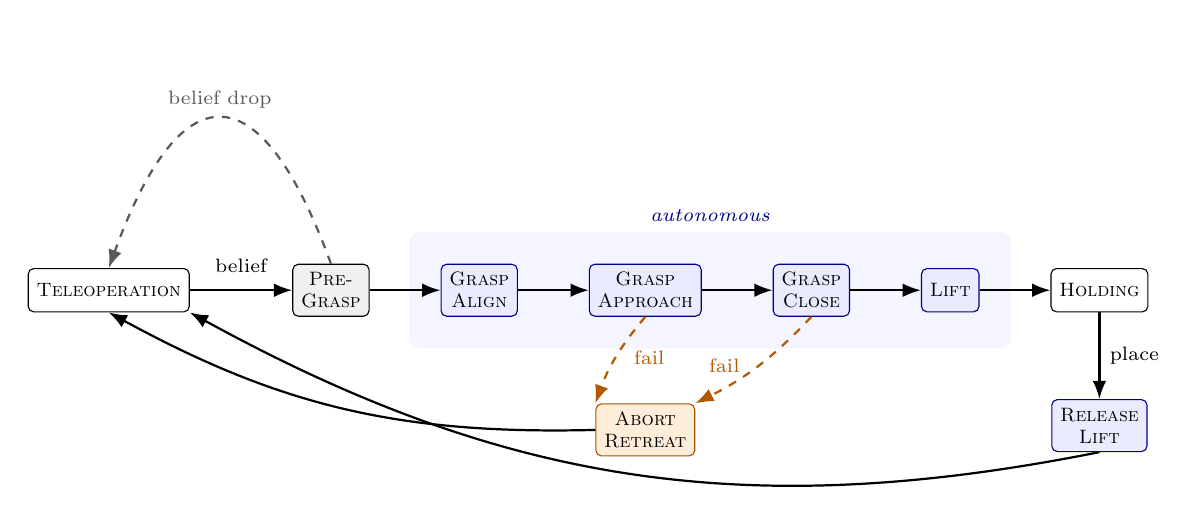
\begin{tikzpicture}[
  font=\scriptsize,
  state/.style={draw, rounded corners=2pt, align=center, inner sep=3pt, minimum height=5.5mm, fill=white},
  auto/.style={state, fill=blue!8, draw=blue!55!black},
  gate/.style={state, fill=gray!12},
  fail/.style={state, fill=orange!15, draw=orange!65!black},
  main/.style={-Latex, thick},
  soft/.style={-Latex, thick, dashed, gray!70!black},
  bad/.style={-Latex, thick, dashed, orange!70!black},
  node distance=4mm and 9mm]
\node[state] (sa) {\textsc{Teleoperation}};
\node[gate, right=13mm of sa] (pg) {\textsc{Pre-}\\\textsc{Grasp}};
\node[auto, right=of pg] (al) {\textsc{Grasp}\\\textsc{Align}};
\node[auto, right=of al] (ap) {\textsc{Grasp}\\\textsc{Approach}};
\node[auto, right=of ap] (cl) {\textsc{Grasp}\\\textsc{Close}};
\node[auto, right=of cl] (li) {\textsc{Lift}};
\node[state, right=of li] (ho) {\textsc{Holding}};
\node[fail, below=11mm of ap] (ab) {\textsc{Abort}\\\textsc{Retreat}};
\node[auto, below=11mm of ho] (rl) {\textsc{Release}\\\textsc{Lift}};
\begin{pgfonlayer}{background}
\node[fit=(al)(ap)(cl)(li), fill=blue!4, rounded corners=4pt, inner sep=4mm,
      label={[blue!55!black, font=\scriptsize\itshape]above:autonomous}] {};
\end{pgfonlayer}
\draw[main] (sa) -- node[above=1mm]{belief} (pg);
\draw[main] (pg) -- (al);
\draw[main] (al) -- (ap);
\draw[main] (ap) -- (cl);
\draw[main] (cl) -- (li);
\draw[main] (li) -- (ho);
\draw[main] (ho) -- node[right]{place} (rl);
\draw[bad] (ap.south) to[bend right=10] node[right, pos=0.5, xshift=1mm]{fail} (ab.north west);
\draw[bad] (cl.south) to[bend left=10] node[left, pos=0.5, xshift=-1mm]{fail} (ab.north east);
\draw[main] (ab.west) to[bend left=15] (sa.south);
\draw[main] (rl.south) to[bend left=20] (sa.south east);
\draw[soft] (pg.north) to[out=110, in=70, looseness=2.4] node[above]{belief drop} (sa.north);
\end{tikzpicture}}
\caption{Grasp lifecycle. The highlighted chain executes autonomously with boosted tracking; a belief drop or a phase failure both return control to the operator.}
\label{fig:fsm}
\end{figure}

\textbf{Commit and execution.} A single press of the left device button (Section~\ref{sec:opcontrols}) requests a grasp, granted only when the object-level belief $B_{\text{obj}}(o^{\star})$~\eqref{eq:objbelief} and the \emph{measured} gripper pose are both within entry tolerance of the goal standoff, each with hysteresis so noise cannot chatter the state. Reading the real pose rather than the reference forces the operator to bring the arm itself to the standoff before the grasp will trigger. From \textsc{Grasp-Align} to \textsc{Lift} the arm then follows the per-goal robot policy with tracking boosted (Section~\ref{sec:sched}) and belief, blending, and teleoperation suspended; any phase timeout aborts into a retreat that returns authority to the operator.

\textbf{The object in the collision model.} A single ``released pair'' does not describe how the target object actually moves through the collision model; five regimes do, executed as a hybrid automaton rather than a continuous deformation of one constraint:
\begin{itemize}[nosep]
\item \emph{Align/Approach}: the commit event bypasses the gripper--target pair, removing it from the SoftMin outright rather than merely relaxing it; the relaxed margin value set at the same instant stays inert while the pair is absent.
\item \emph{Close}: the fingers-commanded-closed event re-admits the pair at that relaxed margin, a discrete switch with no reset dynamics of its own.
\item \emph{Lift/Holding}: on attach completion the object is re-parented onto the wrist joint, its pairs against the rest of the world become active, and every pair touching it starts from a large positive distance shift that decays over an attach ramp.
\item \emph{Release}: the travel-gated retreat detaches the object to its placed world pose, removes its pairs against the table, ground, and body outright, and re-admits the gripper--object pair under the same positive-shift, decaying-ramp treatment as attach.
\item \emph{Abort recover}: the same travel-gated retreat, following a failed attempt, holds the bypass, then clamps the margin to the live measured contact and, after a debounce, ramps it from the relaxed value back to nominal.
\end{itemize}

The only ramps in the whole lifecycle are the attach/detach distance shift and the abort-recovery margin ramp (Appendix~\ref{app:config} gives their durations and the margin values); the commit-time release is a discrete pair removal, not a ramp, and no ramp derivative enters the enforced row~\eqref{eq:cbf}. Continuity of the margin value smooths the row and its multiplier \emph{within} a regime, but it does not keep the state inside the previous regime's admissible set, since $\mathcal{P}(X)$, and hence $h_{\text{soft},X}$, change discontinuously at every regime boundary above. The mechanism is therefore a smooth heuristic for handing a barrier from one geometry to another, not a preservation of the original collision-free set: invariance is intentionally suspended for the target pair from commit until the object is re-parented at Lift, or until the reactivation ramp completes after the retreat clearance at Release, and it is never suspended for any other declared pair. The physical hardware teleoperation trial reported in this work ran an earlier revision, with a fixed-duration, clearance-blind abort retreat and no Recover phase.

%───────────────────────────────────────────────────────────────────────────────
\section{Haptic interface and force rendering}
\label{sec:teleop}

The operator commands the robot through a grounded six-degree-of-freedom haptic interface of impedance type: it measures handle motion and renders a commanded wrench on the handle (the devices used are described in Section~\ref{sec:hardware}). This section gives the frame convention, the two command mappings that turn handle motion into an arm reference, and the force laws that determine every wrench rendered on the handle, with and without assistance.

\subsection{Device frame and driver-side wrench}
\label{sec:device}

\textbf{Frame convention.} The device reports handle motion, and receives the commanded wrench, in its own base frame, which the driver leaves at the manufacturer's native convention; that frame does not coincide with the robot base frame. This work relates the two by a pure $180^{\circ}$ rotation about the vertical axis, $\Phi = R_z(\pi) = \operatorname{diag}(-1,-1,1)$. The rotation is a design choice of the teleoperation layer, not a property of either device: it makes the gripper move in the direction the hand moves for an operator who faces the device and watches the robot from behind, so pushing the handle away drives the gripper forward and a sideways motion stays on the same side. $\Phi$ flips the sign of the $x$- and $y$-components of any 3-vector (linear or axial), leaving the vertical component unchanged, and is applied to every quantity crossing between the two frames:
\begin{equation}
v^{\text{robot}} = \Phi\, v^{\text{dev}},
\qquad
F^{\text{dev}} = \Phi\, F^{\text{robot}},
\label{eq:flip}
\end{equation}
and because flipping twice returns the original vector, $\Phi$ undoes itself, so the same flip converts a velocity device $\to$ robot and a wrench robot $\to$ device: one formula, both directions.

\textbf{Operator controls.}
\label{sec:opcontrols}
Discrete commands reach the system through programmable buttons on the handle (Figure~\ref{fig:haptiondevices}), each mapped in software to one command. The right button is the clutch: while it is held the pose reference is frozen (Section~\ref{sec:clutchmode}) and reference blending is suspended (Section~\ref{sec:blend}), so repositioning the hand neither moves the robot nor is read as intent; the joystick mapping needs no indexing and ignores it. The left button is an event channel read by edge detection over a double-press window $T_{\text{dp}}$: a single press requests a grasp (Section~\ref{sec:grasp}), a double press switches the active arm. On the full-size device a deadman switch additionally gates the session, the operator being in control only while holding it.

\textbf{Viscous damping.} Every rendered wrench, in every condition, carries a constant viscous damper $(-K_d^{\text{lin}} v_h,\, -K_d^{\text{ang}} \omega_h)$ opposing handle motion, with $v_h$ and $\omega_h$ the handle linear and angular velocity. Rendering the damper in the assistance process would add a topic hop of delay on top of the sample period, so it is computed at the driver from the same-tick velocity sample and added after the slew limiter, on top of whichever wrench the active force law supplies; same-tick computation removes that delay but does not by itself make a sampled damper passive, a passivity concern taken up with the guidance force below.

\subsection{Clutch mode --- position control}
\label{sec:clutchmode}

Clutch mode is position-control teleoperation with indexing. The handle twist is integrated into a pose reference,
\begin{equation}
p_{\text{ref}} \leftarrow p_{\text{ref}} + \Phi\, v_h\,\Delta t,
\qquad
R_{\text{ref}} \leftarrow \exp_3\!\bigl(\Phi\,\omega_h\,\Delta t\bigr)\, R_{\text{ref}},
\label{eq:clutchint}
\end{equation}
and published with the feed-forward twist consumed by the CLF row~\eqref{eq:clf}. While the clutch is held the reference is frozen and a zero twist is published, so the operator repositions the hand freely and a bounded device yields an unbounded workspace. The map is unscaled: workspace extension comes entirely from indexing, so hand and gripper displacements correspond one to one and the operator's kinaesthetic calibration transfers directly to fine manipulation. The integration anchor is the measured end-effector pose, re-captured on every arm switch and at the end of every autonomous phase, so teleoperation always resumes from where the robot physically is --- no jump, regardless of what the autonomous phase does.

\subsection{Joystick mode --- velocity control}
\label{sec:joystick}

Joystick mode is an alternative teleoperation mapping whose advantage is structural and holds for any device or robot: because the robot is commanded a velocity rather than an integrated position, no clutch is needed to reach the full workspace. The only persistent force on the handle is a centring spring toward a home pose, defined below with the base force per mapping, and intent is read purely as displacement from home. Releasing the handle recentres it, which is exactly a zero command. The two modes are the two classical families of master kinematic mapping, position control and rate control~\cite{kim1987comparison}, and constitute the control-mode factor manipulated in the user study.

With the radial deadband operator
\begin{equation}
\operatorname{db}_{\varepsilon}(d) \;=\;
\begin{cases}
0, & \|d\| \le \varepsilon,\\[2pt]
\dfrac{\|d\|-\varepsilon}{\|d\|}\, d, & \|d\| > \varepsilon,
\end{cases}
\label{eq:db}
\end{equation}
a shrink, with direction preserved and continuous at its boundary, of a raw displacement $d$ past a deadband radius $\varepsilon$, so that diagonal commands are not distorted as they are by per-axis deadbands. The commanded twist is proportional to the displacement past the deadband, lightly damped by the handle velocity, magnitude-clamped, and frame-flipped,
\begin{equation}
\begin{aligned}
v_{\text{user}} &= \Phi\,\operatorname{clamp}_{V_{\max}}\!\Bigl(K_t\,\operatorname{db}_{\varepsilon_{\text{lin}}}\!\bigl(p_h - p_{\text{home}}\bigr) \;-\; c_v\, v_h\Bigr),\\
\omega_{\text{user}} &= \Phi\,\operatorname{clamp}_{\Omega_{\max}}\!\Bigl(K_r\,\operatorname{db}_{\varepsilon_{\text{ang}}}\!\bigl(\log_3(R_h R_{\text{home}}^{\top})\bigr) \;-\; c_\omega\, \omega_h\Bigr),
\end{aligned}
\label{eq:jtwist}
\end{equation}
where $p_h, R_h$ are the handle's measured position and orientation, and $v_h, \omega_h$ its linear and angular velocity as in Section~\ref{sec:device}; $p_{\text{home}}, R_{\text{home}}$ are the home position and orientation, the latter derived below in~\eqref{eq:homerot}; $\varepsilon_{\text{lin}}, \varepsilon_{\text{ang}}$ the linear and angular deadband radii of~\eqref{eq:db}; $K_t, K_r$ the translational and rotational gains; $c_v, c_\omega$ the linear and angular damping coefficients; and $V_{\max}, \Omega_{\max}$ the resulting speed clamps (Appendix~\ref{app:config}). The damping is active only outside the deadband, so a handle resting or settling near home commands exactly zero. The deadband is sized above the centring spring's settling precision, so residual settling motion is never read as input.

The home position is fixed; the home orientation tracks the gripper, so that a handle at rest always means ``hold the current gripper orientation'',
\begin{equation}
R_{\text{home}} \;=\; \exp_3\!\Bigl(\tfrac{1}{s_r}\,\Phi \log_3\!\bigl(R_{\text{EE}}\,\bar{R}_{\text{arm}}^{\top}\bigr)\Bigr)\, R_0,
\label{eq:homerot}
\end{equation}
where $R_0$ is the neutral handle orientation, $\bar{R}_{\text{arm}}$ a per-arm gripper reference captured once at that arm's first activation and never re-anchored, and $s_r > 1$ compresses the gripper's excursion into the device's narrower, unevenly-ranged rotational workspace, the binding constraint on the hand-to-gripper map. The compression applies to the home pose only, never to the commanded twist. Because~\eqref{eq:homerot} is recomputed every tick, including while teleoperation is suspended, the home stays synchronised with the gripper and no state transition produces a jump; the same live home pose is the spring target defined below with the base force per mapping, and the zero point of~\eqref{eq:jtwist}.

Without blending the twist is integrated into a latched reference whose lead over the end-effector is bounded by projection,
\begin{equation}
\|p_{\text{ref}} - p_{\text{EE}}\| \le L_{\text{lin}},
\qquad
\bigl\|\log_3\!\bigl(R_{\text{ref}} R_{\text{EE}}^{\top}\bigr)\bigr\| \le L_{\text{ang}},
\label{eq:latchlead}
\end{equation}
with $L_{\text{lin}}, L_{\text{ang}}$ the maximum allowed linear and angular lead (Appendix~\ref{app:config}), so the reference cannot run away while the arm saturates against a constraint, and on release the arm catches up by at most the cap. With blending the pure user twist is passed to the arbitration law~\eqref{eq:blend} with the live end-effector pose as the belief anchor, $T_{\text{user}} \equiv T_{\text{EE}}$.

\subsection{Force rendering}
\label{sec:rendering}

Every wrench rendered on the handle is the superposition of a base layer, fixed by the control mode, and an assistance layer, fixed by the condition, with two invariants that hold in every condition: the superposed wrench is proportionally rescaled whenever its magnitude exceeds the authority cap $(F_{\text{cap}}, \tau_{\text{cap}})$, preserving direction and layer proportions so that the autonomy can never overpower the operator, and the published wrench is clipped to the device envelope. Writing every wrench as $w = (F, \tau) \in \mathbb{R}^6$, the wrench the operator feels is
\begin{equation}
w_h \;=\; \operatorname{clip}_{\text{dev}}\Bigl(\mathcal{S}_{\text{cap}}\bigl(w_{\text{base}}^{(m)} + a_F\,w_{\text{guide}}\bigr) + w_{\text{cue}}\Bigr) \;-\; \begin{bmatrix} K_d^{\text{lin}}\,v_h \\ K_d^{\text{ang}}\,\omega_h \end{bmatrix},
\label{eq:wtotal}
\end{equation}
with $\mathcal{S}_{\text{cap}}(F, \tau) = \bigl(F\min(1, F_{\text{cap}}/\|F\|),\; \tau\min(1, \tau_{\text{cap}}/\|\tau\|)\bigr)$ the proportional rescale, and the last term the driver-side damper of Section~\ref{sec:device}. The two layers are:
\begin{itemize}[nosep]
\item $w_{\text{base}}^{(m)}$, the base force of the control mode $m \in \{\text{C}, \text{J}\}$, present in every condition and defined in Section~\ref{sec:columnbase},
\begin{equation}
w_{\text{base}}^{(\text{J})} = \begin{bmatrix} F_{\text{home}} \\ \tau_{\text{home}} \end{bmatrix},
\qquad
w_{\text{base}}^{(\text{C})} =
\begin{cases}
\begin{bmatrix} F_{\text{sync}}^{\text{lin}} \\ \tau_{\text{sync}} \end{bmatrix}, & \text{clutch released},\\[10pt]
\begin{bmatrix} 0 \\ \tau_{\text{align}} \end{bmatrix}, & \text{clutch held};
\end{cases}
\label{eq:wbase}
\end{equation}
\item $a_F\,w_{\text{guide}}$, the guidance force of Section~\ref{sec:guidance}, where $a_F \in \{0, 1\}$ is the assistive-feedback factor of the condition: $a_F = 1$ in CF, CFB, JF, and JFB, and $a_F = 0$ in CB and JB (Table~\ref{tab:cells}), whose assistance acts on the reference alone.
\end{itemize}
Two regimes override~\eqref{eq:wtotal}. While the clutch is held, the alignment torque is the whole wrench, with no guidance and no cap, since the operator is repositioning the hand rather than commanding the robot. During autonomous grasp execution the clutch mapping renders no force at all, $w_{\text{base}}^{(\text{C})} = w_{\text{guide}} = 0$, while the joystick mapping keeps its centring spring, which there holds a zero command. The term $w_{\text{cue}}$ collects the vibrotactile cues described with each base force; it carries torque only and is added after the cap, so it is never absorbed by the rescaling.

The two mappings are constructed as duals of one another, so that the assistance factor is compared on equal footing rather than against two unrelated baselines. Each has one base force whose role is to restore the device to its rest relation with the robot. In the joystick mapping a centring spring returns the handle to the deadzone, where the commanded twist is zero; in the clutch mapping a coupling force --- the position-error feedback of a position--position bilateral scheme~\cite{hokayem2006bilateral}, which synchronises handle and robot --- draws the handle, and with it the integrated reference, back toward the robot's actual pose. Each likewise keeps the operator's wrist aware of the gripper's orientation, without which neither mapping is usable at the wrist: the joystick home orientation tracks the gripper continuously~\eqref{eq:homerot}, so that a handle at rest means ``hold the current gripper orientation'', and the clutch mapping renders, whenever the clutch is held, an alignment torque that turns the handle toward the gripper~\eqref{eq:aligntorque}. And in both mappings the guidance force, introduced next, is rendered against that same base force: to follow the guidance the operator moves with it against the spring or the coupling, and to refuse it they move against both. The assistance is thus measured in the same currency in both mappings --- as a fraction of the force that holds the device back --- which is what lets a difference between the two be attributed to the mapping itself rather than to the feel of the assistance.

\subsection{Base force per mapping}
\label{sec:columnbase}

\textbf{Clutch mapping.} The base layer is the coupling force of the position--position scheme, a tether along the robot's tracking error, so the operator feels how far the arm lags its reference:
\begin{equation}
F_{\text{sync}}^{\text{lin}} = K_p^{s}\,\Phi\bigl(p_{\text{EE}} - p_{\text{ref}}\bigr),
\qquad
\tau_{\text{sync}} = K_R^{s}\,\Phi \log_3\!\bigl(R_{\text{EE}}\,R_{\text{ref}}^{\top}\bigr),
\label{eq:fsync}
\end{equation}
with no damping of its own, viscosity being supplied once by the driver-side damper of Section~\ref{sec:device}. The tether target is the published arm reference, which under blending is the blended reference --- the gripper the operator is actually watching.

While the clutch is held the tether is released and the rendered wrench carries an orientation-alignment torque alone: the operator repositions the hand freely in translation while the wrist is drawn into alignment with the gripper. The target is not an absolute orientation but a difference referred to two references, $R_{\text{EE},0}$ and $R_0$, pinned once at the end of the startup homing procedure to the gripper's and the handle's own orientation at that moment,
\begin{equation}
\delta \;=\; \log_3\!\bigl(R_{\text{EE}}\,R_{\text{EE},0}^{\top}\bigr),
\qquad
R_{\text{target}} \;=\; \exp_3\!\bigl(\Phi\,\delta\bigr)\, R_0,
\label{eq:clutchalign}
\end{equation}
where $\delta$ is the gripper's rotation measured from the moment $R_{\text{EE},0}$ is pinned, and $R_{\text{target}}$ applies that same rotation, mapped into the device frame by $\Phi$, to the handle's own pinned orientation $R_0$ --- the orientation the torque below servos the handle toward. Pinning both references once, rather than re-reading them every tick, is mandatory: the gripper's and the handle's zero orientations are unrelated, so only differences transfer between the frames, and position control integrates orientation purely incrementally through~\eqref{eq:clutchint}. Mapping the rotation \emph{vector} through $\Phi$, rather than forming a matrix product across frames and repairing the torque afterwards, is what keeps the result a genuine rotation in the destination frame. Writing $R_h$ for the live handle orientation, the torque is a rotational spring on the residual $e_a = \log_3\!\bigl(R_{\text{target}}\,R_h^{\top}\bigr)$, saturated on its magnitude with its axis preserved,
\begin{equation}
\tau_{\text{align}} \;=\; M_a \tanh\!\Bigl(\frac{K_a\,\| e_a \|}{M_a}\Bigr)\,\frac{e_a}{\| e_a \|},
\label{eq:aligntorque}
\end{equation}
with $K_a$ the angular stiffness and $M_a$ the torque bound. The torque fades to zero within a margin of any device joint limit. Two vibrotactile cues complete the mapping, both a flat torque of fixed small amplitude whose sign reverses every tick, present exactly while their trigger holds: one while any device joint sits within a margin of its limit, one throughout autonomous grasp execution.

\textbf{Joystick mapping.} The base layer is a centring spring toward the live home pose~\eqref{eq:homerot}:
\begin{equation}
F_{\text{home}} = K_P\bigl(p_{\text{home}} - p_h\bigr),
\qquad
\tau_{\text{home}} = K_R \log_3\!\bigl(R_{\text{home}}\,R_h^{\top}\bigr).
\label{eq:fhome}
\end{equation}
$p_{\text{home}}$ is fixed, but $R_{\text{home}}$ is recomputed every tick from the live gripper orientation~\eqref{eq:homerot}, so this is also the orientation-synchronisation mechanism, deliberately rendering no end-effector position tether --- coupling a robot-state force onto the handle whose displacement is then re-read as intent is the loop joystick mode exists to break. The rotation mechanism is structurally the clutch mapping's own delta map~\eqref{eq:clutchalign}: a rotation relative to a reference pinned once, mapped into the device frame by $\Phi$. Two differences follow from the mappings' own structure rather than from the mechanism itself: the reference $\bar{R}_{\text{arm}}$ is pinned at that arm's first activation rather than at startup homing, and the delta is compressed by $1/s_r$ into the device's narrower rotational range, since joystick mode has no indexing step to periodically reset how far it has drifted the way clutching does. Its magnitude therefore differs from the clutch tether by design: the two mappings define their base feedback differently, and that difference is part of the manipulated factor. The same vibrotactile cue signals the handle being outside either deadband, so the operator always feels when a command is being impressed, and signals autonomous grasp execution; no follow force accompanies the latter.

\subsection{Guidance force}
\label{sec:guidance}

In the assistive-feedback conditions the inferred intent is rendered as a feed-forward velocity-field force, a guidance virtual fixture~\cite{rosenberg1993virtual,abbott2007haptic}. The belief-weighted blend of the user-frame policies, the same weighting as in~\eqref{eq:blend}, is mapped into the device frame and saturated,
\begin{equation}
v_{\text{field}} \;=\; \Phi\!\sum_{k \in \mathcal{G}_{\text{act}}} b_k\, \pi_k^{\text{user}},
\qquad
F_{\text{guide}} \;=\; g \cdot
\begin{bmatrix}
M_F \tanh\!\bigl(D_F\, v_{\text{field}}^{\text{lin}} / M_F\bigr)\\[2pt]
M_\tau \tanh\!\bigl(D_\tau\, v_{\text{field}}^{\text{ang}} / M_\tau\bigr)
\end{bmatrix},
\label{eq:fguide}
\end{equation}
low-pass filtered for $C^0$ continuity across belief transitions. The gain $g \in [0,1]$ is the product of two smoothstep gates, identical in every guidance condition of both control modes, built from the smoothstep~\eqref{eq:smoothstep}. The confidence gate rises with the active-goal belief $b_{\max} = \max_k b_k$ between $c_{\text{lo}}$ and $c_{\text{hi}}$; the proximity gate falls with distance to the goal, full at $d_{\text{near}}$ and silent from $d_{\text{far}}$ on, so guidance stays off until the operator has brought the reference close enough for the goal manifold to be stable,
\begin{equation}
g \;=\; \sigma\!\bigl(b_{\max};\, c_{\text{lo}}, c_{\text{hi}}\bigr)\;\cdot\;\sigma\!\bigl(\|p_{\text{ref}} - p_{g^{\star}}\|;\, d_{\text{far}}, d_{\text{near}}\bigr).
\label{eq:guidegate}
\end{equation}
Gating on $b_{\max}$, rather than on a peakedness measure such as normalised entropy, which is goal-count dependent, lets every condition share one belief function and one set of margins.

Three properties of~\eqref{eq:fguide} are structural. It is feed-forward, not velocity feedback: the form $D\,(v_{\text{field}} - v_{\text{handle}})$ is a virtual damper whose coefficient, at useful force levels, far exceeds what an impedance loop at $f_{\text{dev}}$ can render passively~\cite{colgate1994factors}; dropping the handle-velocity term turns the guidance into a bias shifting the equilibrium of the base spring rather than a velocity-feedback loop, and the force still vanishes at the goal since $\pi_k \to 0$. No passivity or stability analysis of the complete rendering loop is carried out. The sampled-spring passivity condition $b > KT/2 + |B|$~\cite{colgate1997schenkel}, with $b$ the device's physical damping, $K$ and $B$ the rendered stiffness and damping, and $T = 1/f_{\text{dev}}$ the sample period, cannot be verified because $b$ is not characterised, and it covers only a fixed spring with a same-tick damper, not the moving targets, latency, and saturations of the full loop. No instability was observed across the study and hardware trials. The gain $g$ is applied after the saturation, so it reads directly as a fraction of the guidance authority. And in the joystick mapping the saturations are tied to the deadzone-exit force, the force needed to push the resting handle exactly to the deadband boundary,
\begin{equation}
M_F = \kappa\,\sigma_{\text{lin}}\, K_P\, \varepsilon_{\text{lin}},
\qquad
M_\tau = \kappa\,\sigma_{\text{ang}}\, K_R\, \varepsilon_{\text{ang}},
\qquad
\kappa\,\sigma_{(\cdot)} < 1,
\label{eq:kappacal}
\end{equation}
where $\kappa \in (0,1)$ is the deadzone-exit fraction and $\sigma_{\text{lin}}, \sigma_{\text{ang}} > 1$ per-channel trims. The constraint $\kappa\,\sigma_{(\cdot)} < 1$ is what keeps the guidance a strict bias: below unity it can never push the handle out of the deadband on its own, so the operator remains the sole initiator of motion. In the clutch mapping the saturations are absolute, sized against the sync-tether landscape (Appendix~\ref{app:config}).

%───────────────────────────────────────────────────────────────────────────────
\section{Head perception and the camera-derived world model}
\label{sec:head}

The 7-DOF head carries an RGB-D camera and serves two roles: framing the operator's active hand during teleoperation, and building the collision world autonomously.

\subsection{Active-arm visual servoing (teleoperation)}
\label{sec:headtrack}

During teleoperation the head keeps the operator's active hand framed, tracking the grasp frame of the active gripper --- the same frame the safety QP, the belief estimator, and the grasp state machine treat as the hand. The head is driven by its own QP, sharing no decision variable with the arm controller, over $x_h = [\qdot_h \in \mathbb{R}^7,\, s \in \mathbb{R}^3]$, solved every control tick as
\begin{equation}
\label{eq:headqp}
\begin{split}
\min_{\qdot_h,\,s} \;\;
&\underbrace{\sum_{i=1}^{7}\lambda_{h,i}\bigl(\qdot_{h,i}-\qdot_{h,i}^{\text{ref}}\bigr)^2}_{\text{posture + lean}}
\;+\; \underbrace{s^{\top}W_s\,s}_{\text{visual slack}} \\
&\;+\; \underbrace{w_{\text{roll}}\bigl(J_{\text{roll}}\qdot_h-\omega_{\text{align}}\bigr)^2}_{\text{roll preference}}
\;+\; \underbrace{w_{\text{app}}\,\|J_{\text{lin}}\qdot_h-v_{\text{orbit}}\|^2}_{\text{approach preference}}
\end{split}
\end{equation}
subject to
\begin{align}
J_{\text{task}}\,\qdot_h - s \;&=\; -\lambda_v\, e \label{eq:headtask}\\[2pt]
-\gamma_{\text{fov}}\bigl(m_{\text{fov}}-\zeta\bigr) \;\le\; J_{\zeta}\,\qdot_h \;&\le\; \gamma_{\text{fov}}\bigl((M_{\zeta}-m_{\text{fov}})-\zeta\bigr), \label{eq:headfov}\\[2pt]
&\quad \zeta \in \{u_h, v_h\} \notag \\[2pt]
\bigl[J_{\text{soft},\text{head}}(q)\bigr]_{\mathcal{H}}\,\qdot_{\mathcal{H}} \;&\ge\; \notag\\[-1pt]
&\quad -\,\gamma_{\text{head}}\,\Bigl(h_{\text{soft},\text{head}}(q) - \bigl(d_{\text{safe},\text{head}} + d_{\text{extra}}\bigr)\Bigr) \label{eq:headcbf}\\[2pt]
\qdot_{h,\min,i} \;\le\; \qdot_{h,i} \;&\le\; \qdot_{h,\max,i} \quad \forall i \label{eq:headjl}
\end{align}
Here:
\begin{itemize}[nosep]
\item $\qdot_h^{\text{ref}}$ and $\lambda_{h,i}$, in the cost~\eqref{eq:headqp}: the posture-plus-lean term, combining the same inverse-square joint-limit potential as the arm posture task (Section~\ref{sec:posture}) with a lateral lean pulling the head elbow toward the active hand's side, so the proximal joints, not only the wrist, follow an arm switch; both terms are clamped at a fraction of the velocity cap so neither can claim the whole budget, and near a bound they push the same way as~\eqref{eq:headjl}. $\lambda_{h,i}$ is its uniform per-joint weight. During an arm-switch retraction $\qdot_h^{\text{ref}}$ is instead a joint-space servo toward a compact home configuration, and the roll/approach terms below are dropped, leaving only~\eqref{eq:headcbf} and~\eqref{eq:headjl} active;
\item $s$ and $W_s$, in the cost~\eqref{eq:headqp}: the visual-task slack and its weight --- a pixel weight on the image-plane rows and a scaled-up weight on the depth row so a comparable centimetre of depth error and pixel error are priced alike; re-weighted uniformly when $s$ instead carries angular units (position-based visual servoing (PBVS), below);
\item $J_{\text{roll}}, \omega_{\text{align}}, w_{\text{roll}}$ and $J_{\text{lin}}, v_{\text{orbit}}, w_{\text{app}}$, in the cost~\eqref{eq:headqp}: the roll- and approach-alignment preferences --- camera roll-rate and linear-velocity Jacobian rows, their commanded rates (up-righting the image against the world vertical, and orbiting the camera toward the gripper's approach axis), and their weights, recomputed each tick and gated to vanish smoothly as the hand leaves the optical axis, so neither preference can fight acquisition;
\item $J_{\text{task}}, e, \lambda_v$, in~\eqref{eq:headtask}: the visual task itself, driving the hand toward the image centre at the target stand-off. With the hand inside the field of view (FOV), the controller runs image-based visual servoing (IBVS): $J_{\text{task}}$ is the 2.5D interaction-matrix Jacobian~\cite{malis1999,chaumette2006} and $e = [u_h-u^{\star},\,v_h-v^{\star},\,Z_h-Z^{\star}]$ the stacked pixel-plus-depth error; with the hand outside the FOV, the controller runs PBVS: $J_{\text{task}}$ is the camera's rotational-velocity Jacobian rows and $e$ the angular error rotating the optical axis onto the hand direction;
\item $\gamma_{\text{fov}}, m_{\text{fov}}$, in~\eqref{eq:headfov}: the FOV barrier, holding the hand clear of the image edges (IBVS only) --- barrier gain and the shared pixel margin from every edge. One row per image axis is meant: $\zeta$ ranges over the hand's horizontal and vertical pixel coordinates $\{u_h, v_h\}$, with $J_{\zeta}$ the matching row of $J_{\text{task}}$ ($[J_{\text{task}}]_{1,:}$ for $u_h$, $[J_{\text{task}}]_{2,:}$ for $v_h$, since the predicted pixel rate is exactly what the visual task already computes) and $M_{\zeta}$ the matching image dimension ($W_{\text{im}}$ for $u_h$, $H_{\text{im}}$ for $v_h$);
\item $\mathcal{H}, \qdot_{\mathcal{H}}, \gamma_{\text{head}}, d_{\text{safe},\text{head}}, d_{\text{extra}}$, in~\eqref{eq:headcbf}: the head-vs-arm collision barrier, detailed below;
\item $\qdot_{h,\min,i}, \qdot_{h,\max,i}$, in~\eqref{eq:headjl}: the head's own instance of the joint-limit velocity CBF of Section~\ref{sec:jl}.
\end{itemize}
The rate at which the visual error is driven down is set jointly by $\qdot_{\max}$ and $\lambda_v$,
\begin{equation}
\dot{s} \;=\; \min\!\bigl(\qdot_{\max},\; \lambda_v\,\|e\|\bigr),
\label{eq:headvel}
\end{equation}
flat at $\qdot_{\max}$ for $\|e\| > \qdot_{\max}/\lambda_v$ and exponential at rate $\lambda_v$ below it, so the cap owns the far field and the gain the near field. An active-arm switch retracts the head to its home configuration under the head-CBF and joint-limit rows alone, so re-entry into tracking never begins from a stretched chain.

\textbf{Head-vs-arm collision barrier.} The safety QP carries the head chain as a quasi-static obstacle, but its dynamic margin~\eqref{eq:dsafe} thickens with the arm's own joint-velocity norm only, so a moving head acts on that barrier as an unmodelled disturbance. The head QP supplies the symmetric half from the arms' own barrier: the SoftMin aggregation of~\eqref{eq:softmin} is taken over $\mathcal{P}(\text{head})$, the active pairs that touch a head capsule, giving row~\eqref{eq:headcbf} above, where $d_{\text{safe},\text{head}} = d_0 + k_v\,\|\qdot_{\mathcal{H}}^{-}\|$ is of the form~\eqref{eq:dsafe} but driven by the head velocity commanded on the previous tick, precisely the term the arm-side margin lacks, so the same unit correction and the same bound~\eqref{eq:tauv} apply, with $r_{\max}$ for the head chain of the same order as the arm's, giving a comparable $\tau_v$. With a lower gain and an extra margin, the head brakes sooner and more softly than the arm for the identical encounter, so a close call is paid for in camera-tracking performance rather than in arm task performance; the arm's own barrier on the same pair is untouched. If the appended row is infeasible against the joint-limit box, the head is commanded zero velocity: it freezes rather than colliding.

\subsection{Autonomous scene perception and world-model freezing}
\label{sec:convergence}

Independently of teleoperation, the head can build the collision world of Section~\ref{sec:task} from its own depth stream. The table plane is fitted by RANSAC~\cite{fischler1981ransac}, the points above it are clustered, and each cluster's rim is fitted by a circle to give the cylinder's centre, radius, and height; estimates are fused over time, and each object carries an \emph{arc coverage} recording which sectors of its circumference have been observed. Head motion is led by perception: fixation targets are chosen to raise the coverage of the least-covered object, frames are fused only while the head is settled, and the policy is bounded by a time budget.

The estimate is handed to the safety controller only when it has demonstrably stopped changing, by a criterion that needs no ground truth. Convergence requires every expected object present above a confidence floor and an arc-coverage floor $c_{\min}$, so that a geometrically insufficient view can never start the clock, and an oscillation-amplitude lock over a sliding window $\mathcal{W}$ of settled frames of duration $T_w$,
\begin{equation}
\max_{t \in \mathcal{W}} \bigl\|c(t) - \bar{c}_{\mathcal{W}}\bigr\| \le \varepsilon_{\text{pos}},
\qquad
\max_{t \in \mathcal{W}} \bigl|r(t) - \bar{r}_{\mathcal{W}}\bigr| \le \varepsilon_{\text{dim}},
\label{eq:amplock}
\end{equation}
with $c(t)$ and $r(t)$ each object's centre and radius, $\bar{c}_{\mathcal{W}}, \bar{r}_{\mathcal{W}}$ their window means, and $\varepsilon_{\text{pos}}, \varepsilon_{\text{dim}}$ the admitted bands; any head-motion frame clears the window, so motion time is never credited as stability. An amplitude band over a window captures slow drift and fast wobble in one frame-rate-independent test, which a per-frame drift counter cannot, since a static but wrong viewpoint passes it trivially. The criterion certifies stationarity, not accuracy: a consistently biased fit, from depth noise, extrinsic calibration, plane fit, segmentation, or circle fit, passes it as readily as an accurate one. None of these error sources is bounded, and no bound is propagated into the barrier; the only buffer against a radius underestimate is $d_0$~\eqref{eq:dsafe}, so a bias larger than that margin is not absorbed. Measurement-robust barrier functions~\cite{cosner2021mrcbf} (Section~\ref{sec:sota-world-representation}) are the principled remedy, left as future work. Hardware accuracy is not measured against ground truth. On convergence the estimate is frozen and published once as a latched snapshot --- table box and cylinders --- which replaces the declared world as the safety controller's collision model, with everything downstream unchanged. The pipeline supports an optional radius inflation, set to zero in every trial reported here, so the frozen model carries each cylinder's raw fitted radius. The world is deliberately not updated per tick: a moving obstacle set would make the barrier non-stationary and void the forward-invariance argument of Section~\ref{sec:cbf}.

%───────────────────────────────────────────────────────────────────────────────

\chapter{Experiments and results}
\label{ch:exp}

\section{Hardware}
\label{sec:hardware}

Every trial in this chapter, from the hardware validation to the simulated user study, runs on the same robot, driven through one of two devices from the same haptic-interface family. This section introduces the physical hardware once, at a high level; the quantitative envelope of the study's own device is tabulated in Appendix~\ref{app:config}.

\subsection{PAL TRIAGo}
\label{sec:hwtriago}

The robot is a PAL Robotics TRIAGo, a bimanual mobile manipulator built around a wheeled base, a lift torso, two 7-DOF arms ending in two-finger grippers, and a 7-DOF sensorised head carrying an RGB-D camera (Figure~\ref{fig:hwtriago}). Every mechanism this thesis controls --- the safety filter of Chapter~\ref{ch:method}, the shared-autonomy arbitration, and the active-vision head servo --- runs on this same kinematic chain, in simulation throughout the study and on the physical unit shown here for the two hardware trials reported in this chapter.

\begin{figure}[t]
\centering
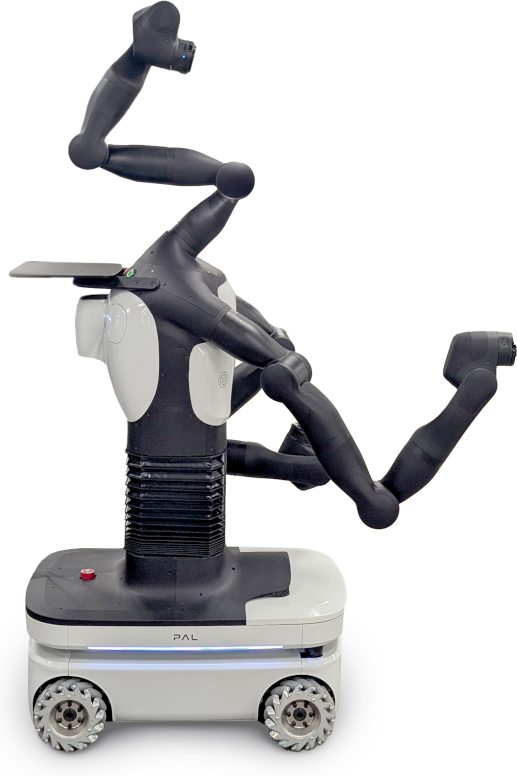
\includegraphics[height=6.8cm]{triago_lateral.png}\hspace{1.5cm}%
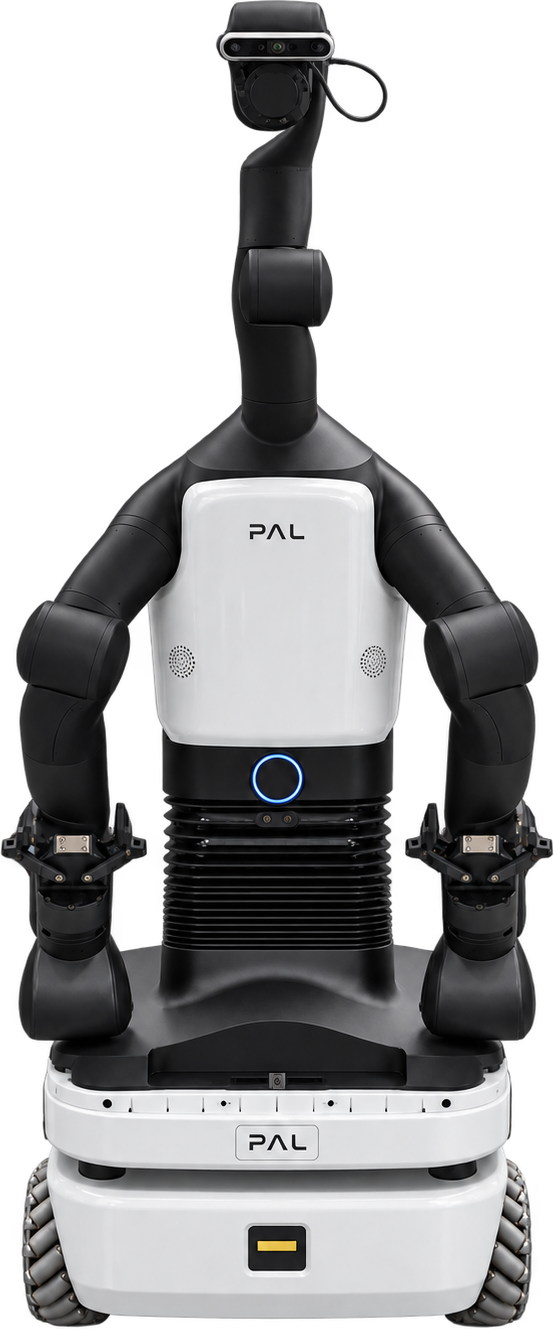
\includegraphics[height=6.8cm]{triago_front.png}
\caption{The physical PAL TRIAGo: a lateral view (left), and a front view in the home configuration the robot assumes at power-on, with the two-finger grippers mounted (right).}
\label{fig:hwtriago}
\end{figure}

\subsection{Haption Desktop 6D Compact}
\label{sec:hwdesktop}

The operator's interface for every session of the simulated study is a Haption Desktop 6D Compact (Figure~\ref{fig:haptiondevices}, left), a benchtop, six-degree-of-freedom impedance-type haptic device: it measures the handle's own pose and renders a commanded wrench back onto it, the mechanism both control mappings of Section~\ref{sec:device} are built on. A push-button pad fitted on the handle (Figure~\ref{fig:haptiondevices}, centre) carries the operator's discrete commands; its buttons are programmable, so each can be mapped in software to an arbitrary command (Section~\ref{sec:opcontrols}). Its joint travel and Cartesian workspace are tabulated in Appendix~\ref{app:config}.

\subsection{Haption Virtuose 6D}
\label{sec:hwvirtuose}

The two hardware trials instead use a Haption Virtuose 6D (Figure~\ref{fig:haptiondevices}, right), the full-size member of the same device family: the same six-degree-of-freedom impedance interface and control software, mounted on a floor-standing pedestal with a substantially larger reach than the desktop unit. The two devices share a control interface but not a physical envelope, so the desktop unit's workspace of Appendix~\ref{app:config} does not describe the operator's workspace in the teleoperated hardware trial. Unlike the desktop unit, it also carries a deadman switch on its handle: the device renders forces only while the switch is held, and the hardware trials count the operator as in control only over those intervals.

\begin{figure}[!t]
\centering
\raisebox{-0.5\height}{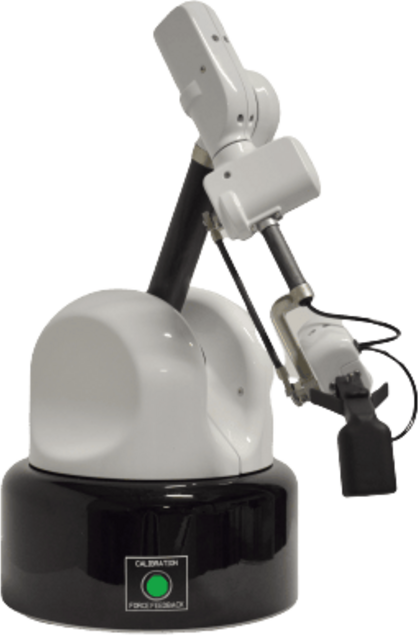
\includegraphics[height=5.1cm]{haption_desktop.png}}\hfill
\raisebox{-0.5\height}{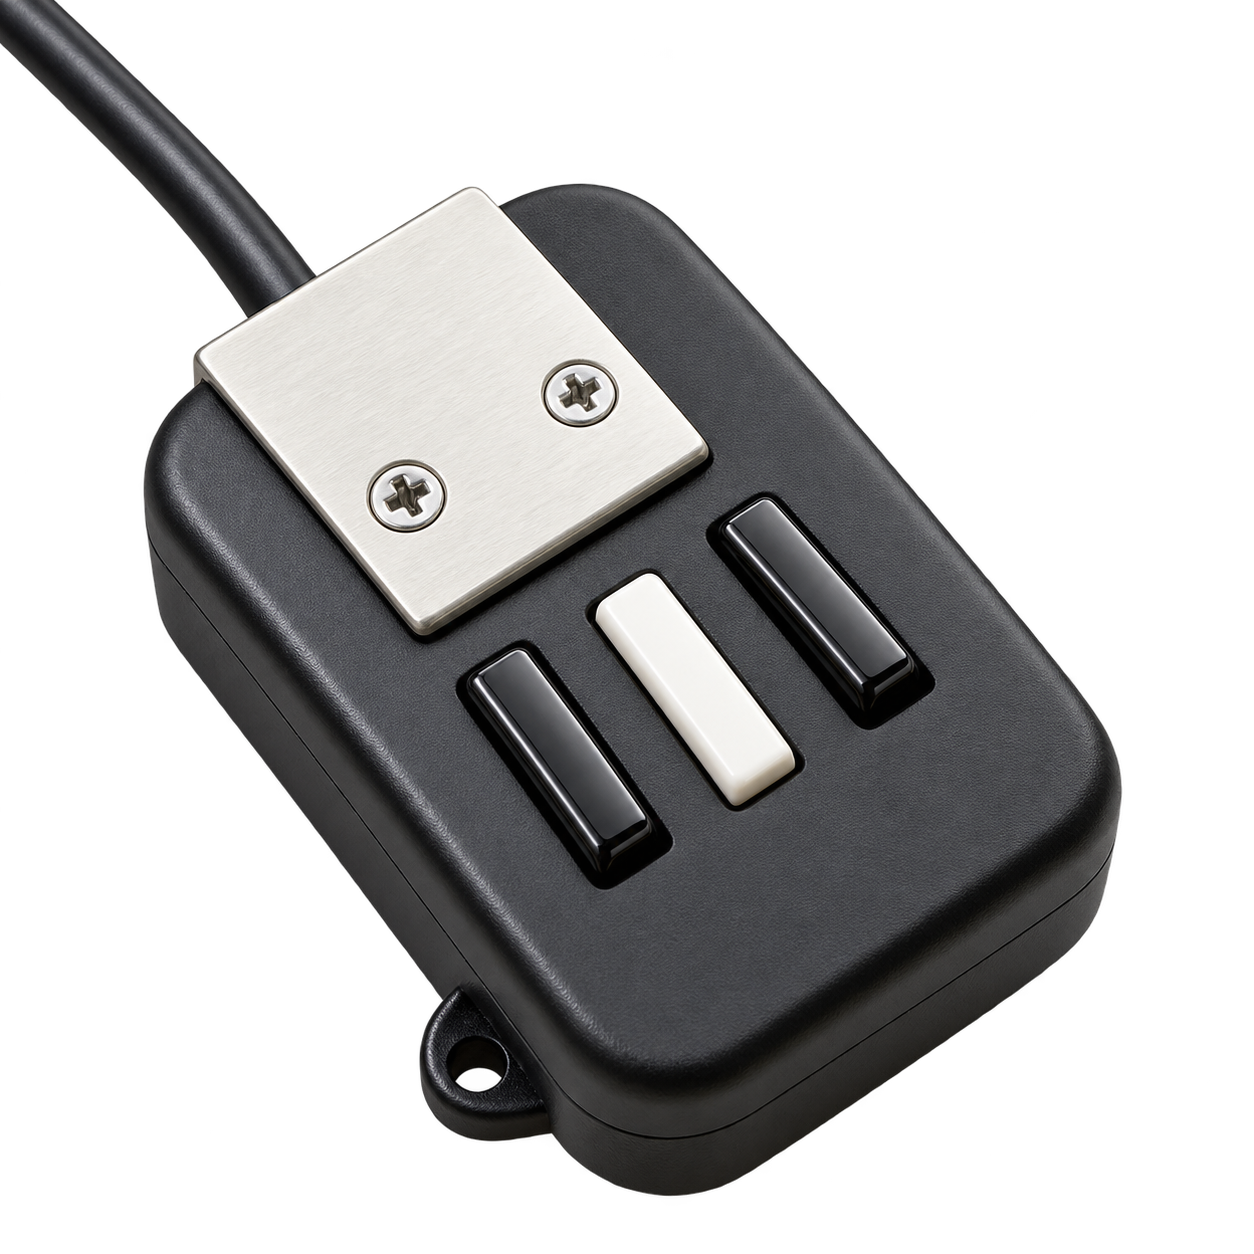
\includegraphics[width=2.9cm]{button.png}}\hfill
\raisebox{-0.5\height}{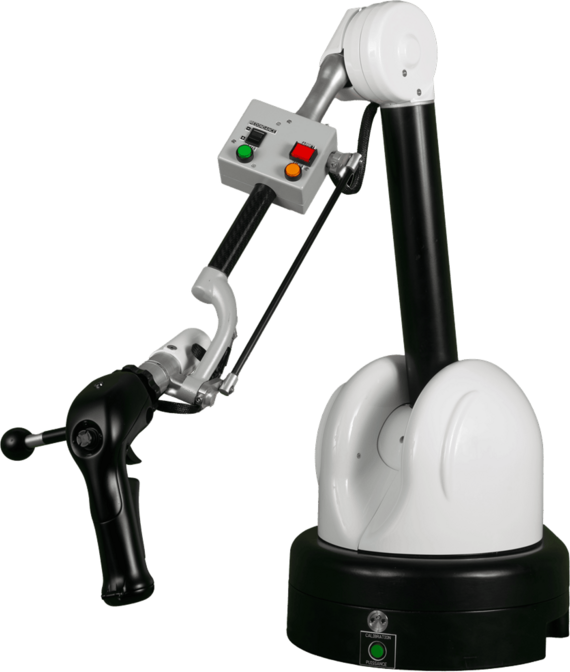
\includegraphics[height=5.39cm]{haption_virtuose.png}}
\caption{The haptic hardware used in this thesis: the Desktop 6D Compact (left) for the simulated study, the programmable push-button pad fitted on its handle, through which the operator issues every discrete command (centre), and the full-size Virtuose 6D (right) for the two hardware trials.}
\label{fig:haptiondevices}
\end{figure}

\FloatBarrier

\section{Hardware validation}
\label{sec:hwvalidation}

The perception pipeline is validated separately on the physical robot. The head scans a table carrying two cups; the table plane and both objects are recovered by the RANSAC-based estimator, and the frozen snapshot is loaded as the safety controller's collision model. Teleoperation and barrier-based obstacle avoidance are then exercised against that perceived model, confirming functional end-to-end operation, from depth stream to enforced constraint, but not the geometric accuracy of the perceived model, which is not measured against ground truth on hardware.

\subsection{Start-to-crossed reaching}
\label{sec:hwswap}

The first hardware test targets the controller alone, with vision excluded from the loop. Both arms are driven open-loop, by the same quintic-timed Cartesian reference source used throughout controller development, from a common starting pose --- both grippers raised and held away from the body (Figure~\ref{fig:hwhome}) --- to the pose sampled from the other arm at the start of the motion, so each arm is commanded straight through the space the other one occupies (Figure~\ref{fig:hwcrossed}). That target pair is not jointly reachable without the self-collision and inter-arm rows of the safety filter (Section~\ref{sec:cbf}) becoming active, so the manoeuvre is posed as a conflict between tracking and safety rather than a compliant reach: it tests whether the CLF's tracking slack yields gracefully under that conflict (Section~\ref{sec:clf}), by exactly as much as each arm's adaptively scheduled weight (Section~\ref{sec:sched}) allows, so the controller settles on the best pose the hard constraints admit for both grippers rather than stalling or violating one.

\begin{figure}[t]
\centering
\begin{subfigure}[t]{0.46\linewidth}\centering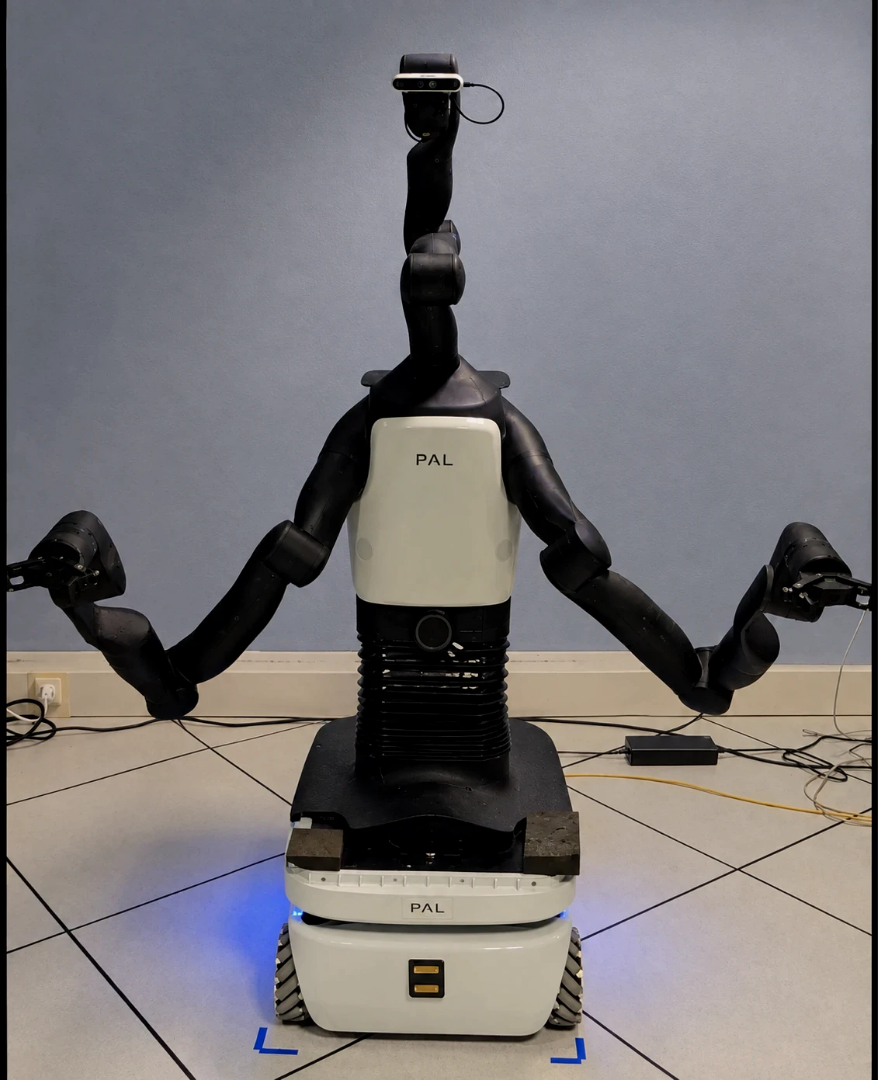
\includegraphics[width=\linewidth]{TRIAGO_Home_Colored.png}\caption{Starting pose}\label{fig:hwhome}\end{subfigure}\hfill
\begin{subfigure}[t]{0.46\linewidth}\centering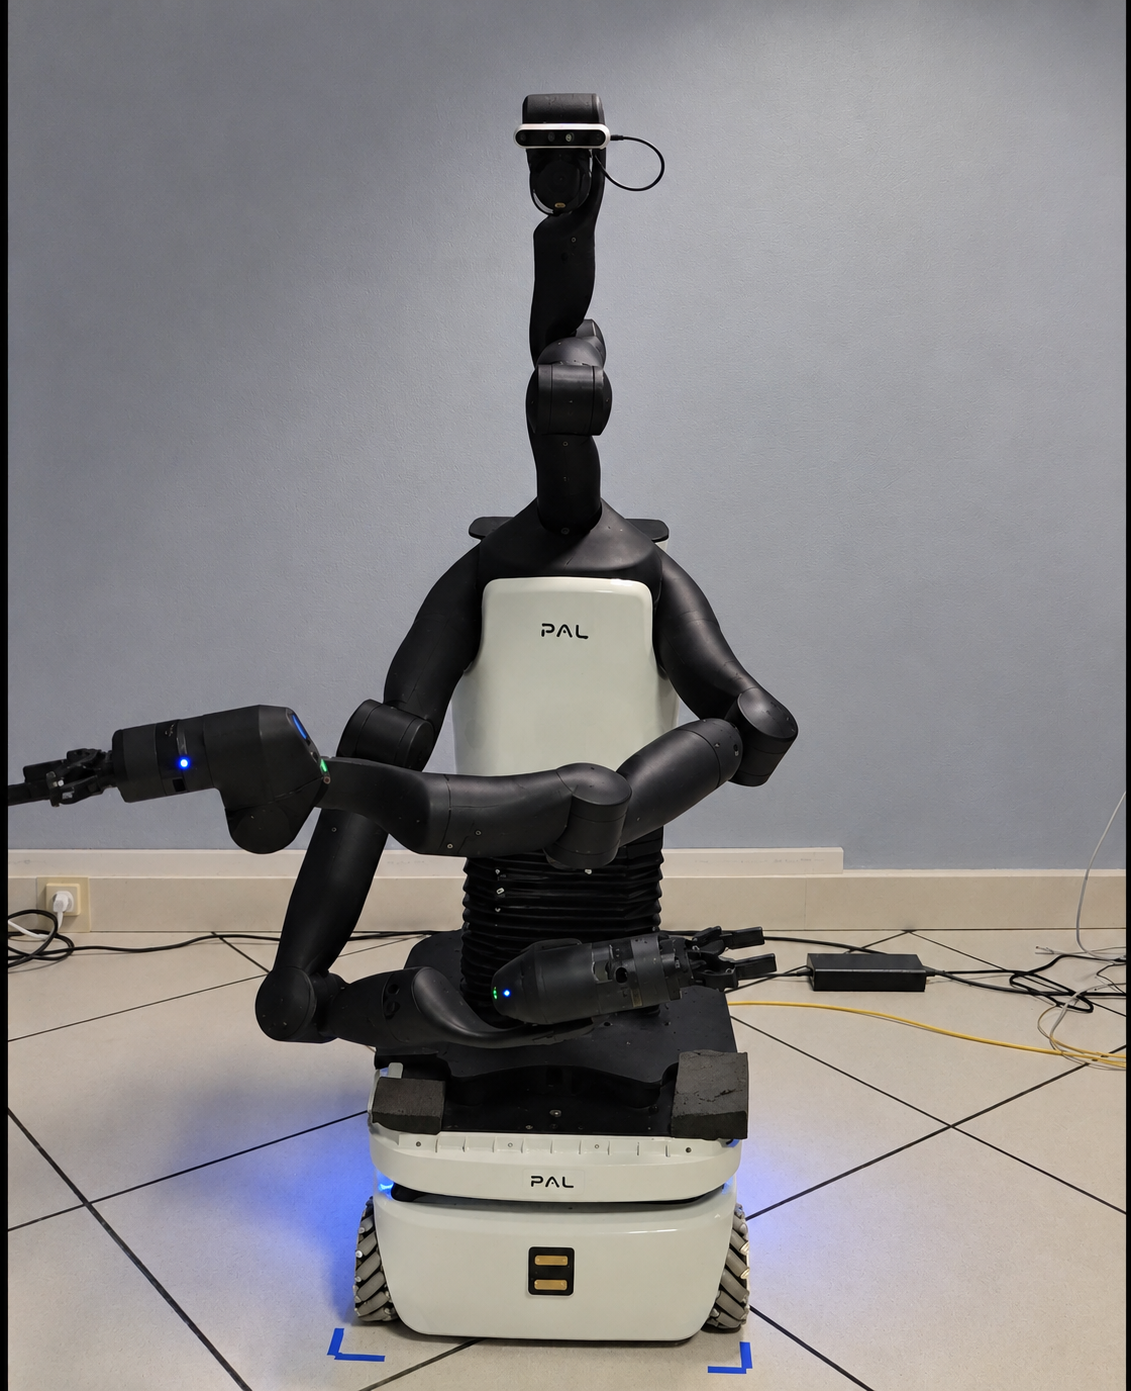
\includegraphics[width=\linewidth]{TRIAGO_Crossed.png}\caption{Crossed configuration}\label{fig:hwcrossed}\end{subfigure}
\caption{The physical robot at the two endpoints of the start-to-crossed reaching test: both grippers start raised and away from the body (left) and finish crossed in front of the torso, each having reached the other's starting pose (right).}
\label{fig:hwswap}
\end{figure}

The manoeuvre is logged with the controller's own telemetry (Section~\ref{sec:sched}), reconstructed offline from the recorded rosbag, over a $25.1$~s trial: the shared quintic-timed reference for both arms runs open-loop from $t=0$ to $t\approx10$~s, marked by the dashed vertical line in every panel of Figures~\ref{fig:hwjoints} and~\ref{fig:hwqpdata}, after which the reference is held fixed at the crossed endpoint for the remainder of the recording. The physical robot sustains a mean loop rate of $126$~Hz with $15.7\%$ tick-to-tick jitter against the $150$~Hz nominal --- lower and noisier than in simulation, as expected on hardware --- with the barrier row computed asynchronously and consumed up to two ticks stale, as Section~\ref{sec:concllimitations} describes. This loop-rate telemetry is a window mean over four control ticks, since the telemetry decimation is doubled on hardware: the window-mean tick period has a median of $7.92$~ms, a 95th percentile of $10.6$~ms, a 99th of $11.7$~ms, and a worst case of $13.6$~ms, with $9.61\%$ of windows exceeding the $6.67$~ms nominal period by more than $50\%$ and $0.132\%$ by more than $100\%$; an independent per-tick estimate, from the barrier-row telemetry published every tick, gives a lower median of $7.58$~ms but a heavier tail, up to $15.8$~ms at the 99th percentile and $19.9$~ms worst case. No exact-zero, infeasible-branch command appears in this trial's $761$ decimated command samples, one in four ticks, which is consistent with the branch's rarity but is not a full-resolution count, and a watchdog freeze is not distinguishable from that branch in the recorded data. Low-level execution is faithful throughout: the root-mean-square mismatch between the commanded and the measured joint velocity, across all 14 arm joints, is $5.0\times10^{-3}$~rad/s, so the discrepancies reported below originate in the constrained optimum the QP is solving, not in how well the robot executes it.

\begin{figure}[t]
\hwjointlegend
\begin{subfigure}[t]{0.485\linewidth}\centering
\includegraphics{results/hw_q_R.pdf}\caption{Joint positions, right arm}\label{fig:hw-qR}\end{subfigure}\hfill
\begin{subfigure}[t]{0.485\linewidth}\centering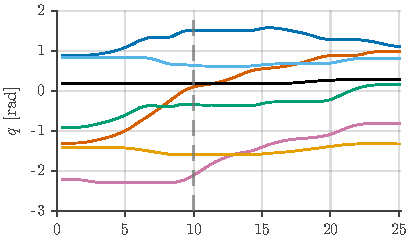
\includegraphics{results/hw_q_L.pdf}\caption{Joint positions, left arm}\label{fig:hw-qL}\end{subfigure}
\vspace{0.3em}
\begin{subfigure}[t]{0.485\linewidth}\centering
\includegraphics{results/hw_qdot_R.pdf}\caption{Measured joint velocities, right arm}\label{fig:hw-qdR}\end{subfigure}\hfill
\begin{subfigure}[t]{0.485\linewidth}\centering
\includegraphics{results/hw_qdot_L.pdf}\caption{Measured joint velocities, left arm}\label{fig:hw-qdL}\end{subfigure}
\caption{Joint-space view of the trial: position and measured velocity of the seven joints of each arm, J1 (shoulder) to J7 (wrist).}
\label{fig:hwjoints}
\end{figure}

Figure~\ref{fig:hwjoints} is the trial seen from the joints. No joint exceeds $0.27$~rad/s at any point, and every velocity trace is smooth: there is no trace of the high-frequency ripple that an unanchored cost otherwise produces on this robot; the measured-velocity rate damping of Section~\ref{sec:rate} suppresses it. The two arms do not stop when the reference does: the joints keep moving after $t\approx10$~s at up to $0.2$~rad/s, slowly and continuously, which is the settling that the shadow prices of Figure~\ref{fig:hwqpdata} account for tick by tick --- the arms are still being moved by the barrier and joint-limit rows, not drifting. The two late joint-limit bursts are visible here as the last inflections of the position traces, around $19$~s on the right arm and $22$~s on the left, after which the configurations settle and the velocities decay to zero.

\begin{figure}[p]
\hwrllegend
\begin{subfigure}[t]{0.485\linewidth}\centering
\includegraphics{results/hw_lambda_cbf.pdf}\caption{CBF shadow price}\label{fig:hw-lcbf}\end{subfigure}\hfill
\begin{subfigure}[t]{0.485\linewidth}\centering
\includegraphics{results/hw_lambda_jl.pdf}\caption{Joint-limit shadow price}\label{fig:hw-ljl}\end{subfigure}
\vspace{0.4em}
\begin{subfigure}[t]{0.485\linewidth}\centering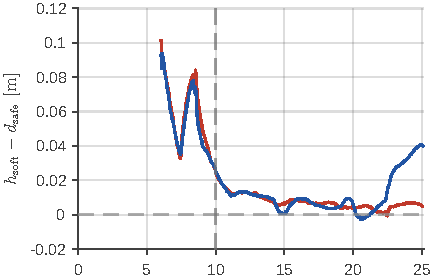
\includegraphics{results/hw_margin.pdf}\caption{CBF safety margin}\label{fig:hw-margin}\end{subfigure}\hfill
\begin{subfigure}[t]{0.485\linewidth}\centering
\includegraphics{results/hw_dmin.pdf}\caption{Minimum inter-geometry distance}\label{fig:hw-dmin}\end{subfigure}
\vspace{0.4em}
\begin{subfigure}[t]{0.485\linewidth}\centering
\includegraphics{results/hw_dsafe.pdf}\caption{Velocity-dependent safety margin}\label{fig:hw-dsafe}\end{subfigure}\hfill
\begin{subfigure}[t]{0.485\linewidth}\centering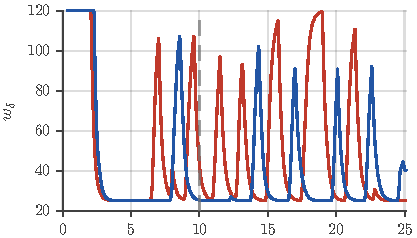
\includegraphics{results/hw_wslack.pdf}\caption{Adaptive slack weight}\label{fig:hw-wslack}\end{subfigure}
\vspace{0.4em}
\begin{subfigure}[t]{0.485\linewidth}\centering
\includegraphics{results/hw_gov_ep.pdf}\caption{Limiter: position error}\label{fig:hw-govep}\end{subfigure}\hfill
\begin{subfigure}[t]{0.485\linewidth}\centering
\includegraphics{results/hw_gov_theta.pdf}\caption{Limiter: orientation error}\label{fig:hw-govtheta}\end{subfigure}
\caption{QP-CLF-CBF and reference-limiter data of the same trial. The vertical axis of (a) is broken between $180$ and $500$ to keep the single $557$ spike in view. Traces (c) and (d) start at $t \approx 6$~s, when the first collision pair enters the activation radius.}
\label{fig:hwqpdata}
\end{figure}

Figures~\ref{fig:hw-lcbf} to~\ref{fig:hw-dsafe} are the safety filter's own account of the conflict. Both collision shadow prices climb together during the transit; the left arm's spikes to the trial's peak of $557$ near $t=6$~s, and both arms show repeated smaller bursts of $100$--$150$ throughout the hold phase, each a fresh barrier engagement rather than one sustained event. That peak and its neighbour are the only two samples above $180$ in the whole trial, so the vertical axis of Figure~\ref{fig:hw-lcbf} is broken between $180$ and $500$: the spike stays visible in the top strip without compressing the bursts that make up the rest of the trace. The joint-limit shadow price is active mainly during the transit, then returns in two brief late bursts, around $19$~s for the right arm and $22$~s for the left. Figures~\ref{fig:hw-margin} and~\ref{fig:hw-dmin} report what those prices are protecting, and both traces likewise only start around this same $t\approx6$~s rather than at $t=0$: both arms begin raised and away from the body and from each other, so no pair is yet within the activation radius (Section~\ref{sec:cbf}), and neither $h_{\text{soft},X}$ nor the raw minimum distance carries a meaningful value against an empty, inactive pair set. From that point on, the CBF safety margin dips to just below zero at its worst ($-2.6$~mm) and otherwise sits within a few millimetres of it for the whole hold phase, while the raw minimum inter-geometry distance floors at $4.2$~cm over the same stretch --- clearance is barrier-limited, the same pattern the human-subject study exhibits at full scale. The velocity-dependent margin $d_{\text{safe},X}$ of~\eqref{eq:dsafe} (Figure~\ref{fig:hw-dsafe}) tracks each arm's own speed directly: it rises to as much as $5.3$~cm during the fast transit and relaxes back toward its $1.5$~cm static floor $d_0$, dotted, as each arm slows.

Figures~\ref{fig:hw-wslack} to~\ref{fig:hw-govtheta} show the two mechanisms that shape what the QP is even asked to do. The slack weight $w_{\delta,X}$ sits at its ceiling before either arm starts moving, collapses to its floor within the first few seconds of motion, and then cycles back toward the ceiling every time that arm's own shadow price relaxes --- the schedule of~\eqref{eq:slacksched}, now read directly from its own output rather than inferred from the slack it produces. Of the reference limiter's four mechanisms (Algorithm~\ref{alg:governor}), only one is exercised by this manoeuvre: the commanded linear speed and angular speed never approach their configured ceilings at any point (not shown), and neither does the orientation-error norm, whose raw and governed traces coincide throughout in Figure~\ref{fig:hw-govtheta} (dashed under solid). Position-error bounding (Figure~\ref{fig:hw-govep}) is the exception, and it is not a brief event: once the right arm's real pose falls behind its raw reference, the governed error is pinned at a common ceiling of about $0.30$~m on $78\%$ of the trial's ticks, and the left arm's error is clamped intermittently over the same stretch it is still converging. The raw traces of the same panel are the residual each arm is left with: at the end of the trial the right gripper sits $0.42$~m and $14.7^{\circ}$ from its commanded pose, the left $0.11$~m and $28.8^{\circ}$ --- each arm converges on a different coordinate of the same target pose, the residual falling wherever its own slack leaves it. This is the same fact the shadow-price and slack panels already show from the QP's side of the loop, seen here from upstream of it: whenever the safety filter is genuinely fighting the reference, the limiter keeps re-issuing one the CLF can still make progress toward, rather than the raw, receding one.

\subsection{Teleoperated bimanual grasping}
\label{sec:hwteleop}

The second hardware trial closes the loop that Section~\ref{sec:hwswap} leaves open: the operator drives the robot directly, through the shared-autonomy architecture of Chapter~\ref{ch:method} rather than an open-loop reference, against the same two-cup tabletop scene introduced at the start of this section. The condition is \textsc{clutch} full guidance (CFB, Table~\ref{tab:cells}): the operator's tether is rendered as both a guidance-biased force on the handle and, through the blending layer, the arm reference itself. The device driving the real robot is a full-size Haption Virtuose 6D, not the Desktop 6D Compact whose joint travel and workspace are tabulated in Appendix~\ref{app:config} for the simulated study --- the two share a control interface but not a physical envelope, so the operator's available motion range in this trial is not the one those tables describe. The trial is recorded over $253.7$~s at a mean loop rate of $109.6$~Hz with $18.6\%$ tick-to-tick jitter, lower and noisier than the open-loop trial of Section~\ref{sec:hwswap} since the shared-autonomy stack now also carries belief estimation, the grasp state machine, and the blending arbitration on every tick. Its window-mean tick period has a median of $9.22$~ms, a 95th percentile of $12.6$~ms, a 99th of $14.6$~ms, and a worst case of $29.4$~ms, with $34.8\%$ of windows exceeding the $6.67$~ms nominal period by more than $50\%$ and $2.51\%$ by more than $100\%$; the per-tick barrier-row estimate gives a median of $8.97$~ms, a 99th percentile of $18.8$~ms, and a worst case of $36.9$~ms. Neither bag records per-tick QP solve times or in-trial end-to-end command latency; a separate transport measurement on the robot network finds a joint-state delay of mean $3.00$~ms, standard deviation $0.12$~ms, a transport figure rather than a sensor-to-actuation latency. The root-mean-square mismatch between commanded and measured joint velocity across all 14 arm joints is $1.2\times10^{-2}$~rad/s, higher than Section~\ref{sec:hwswap}'s $5.0\times10^{-3}$ but still an order of magnitude below the motions it is tracking, so here too execution fidelity is not the limiting factor in what follows.

% NOTE (not for the reader): radius, table footprint, and the blue cylinder's height in fig:telworld are NOT recovered from this trial's own head-perception snapshot (that pipeline doesn't carry them on any topic this bag records) -- they are retrieved from previously recorded values for the same physical rig, reused here for continuity. The PDF text below deliberately does not say this; it states them as retrieved numbers, not as a fresh physical measurement. Keep this distinction in mind if the provenance of these figures is questioned later.
\textbf{World.} The collision model is the head's own live estimate (Section~\ref{sec:convergence}), not a declared one: the trial launches the camera-driven controller variant, which blocks at startup on the head's converged, latched snapshot and never falls back to a static world file. The world holds two cylinders: the red cylinder's top surface sits at $0.872$~m above the base frame, and Figure~\ref{fig:telworld} gives its radius, the table's own footprint, and the blue cylinder's height. The red cylinder sits on the robot's right and the blue on its left, so throughout this section red is the right arm's object and blue the left's, the same colour convention as the arms themselves.

\begin{figure}[t]
\centering

\includegraphics[width=0.92\linewidth]{results/tel_world_recon.pdf}
\caption{Reconstructed two-cylinder world of the trial: top view (left) and front elevation (right). Candidate points are illustrative, not the recorded cloud.}
\label{fig:telworld}
\end{figure}

\begin{figure}[t]
\centering
\begin{subfigure}[t]{0.30\linewidth}\centering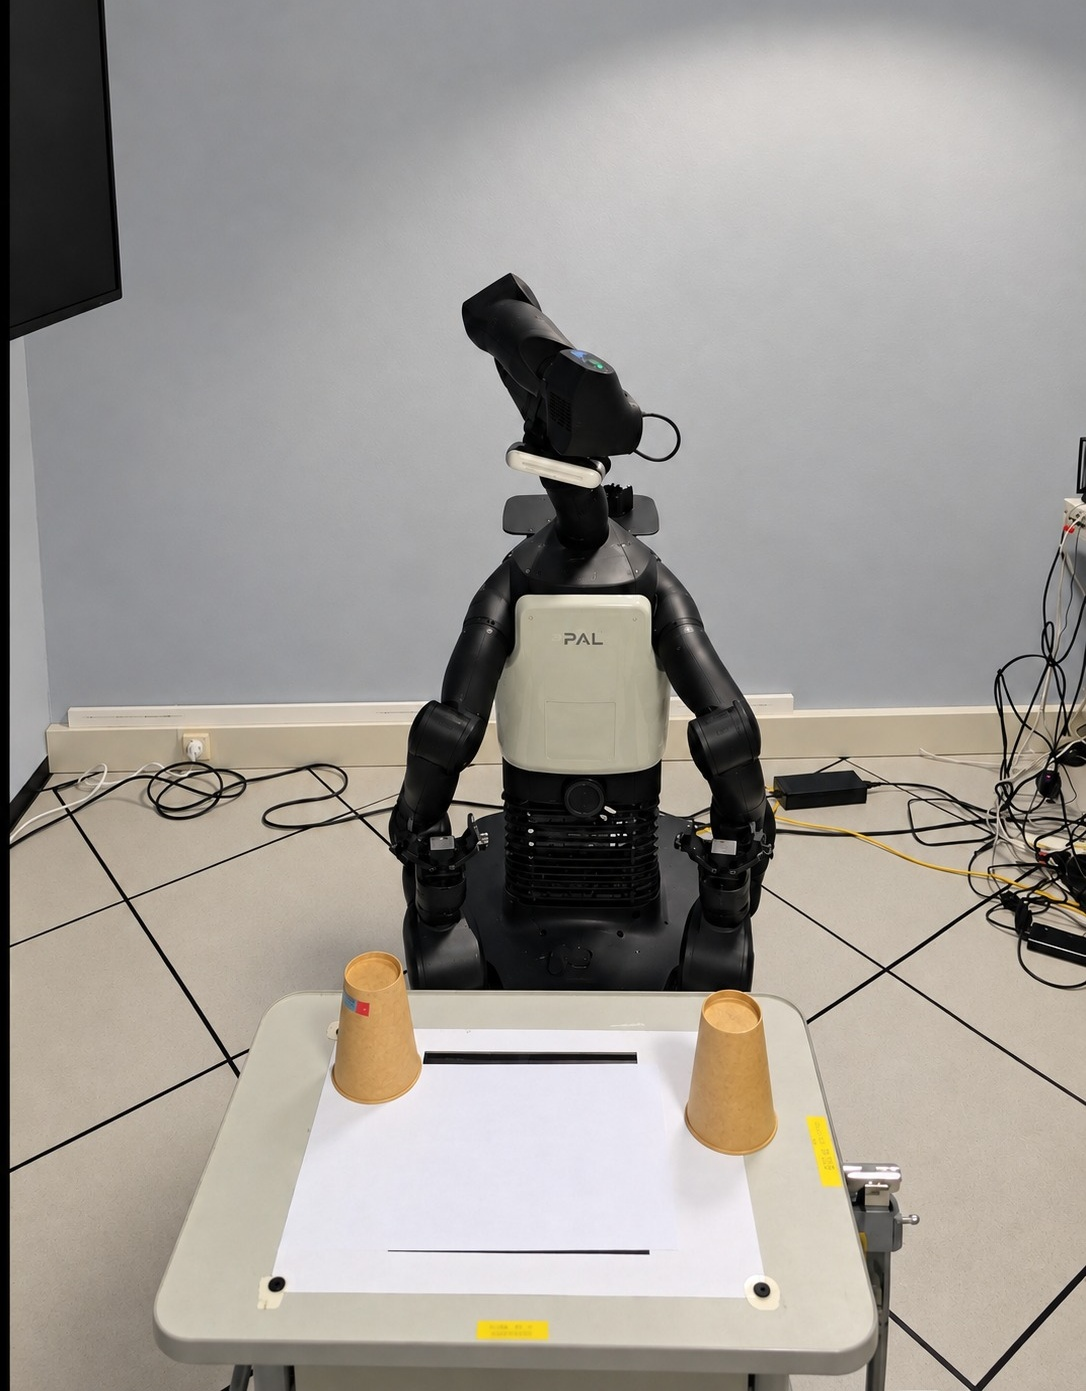
\includegraphics[width=\linewidth]{results/Real_Teleop_10_CFB_SUCCESS/Teleop1_crop.jpeg}\caption{Home configuration}\label{fig:tel-p1}\end{subfigure}\hspace{1.5em}%
\begin{subfigure}[t]{0.30\linewidth}\centering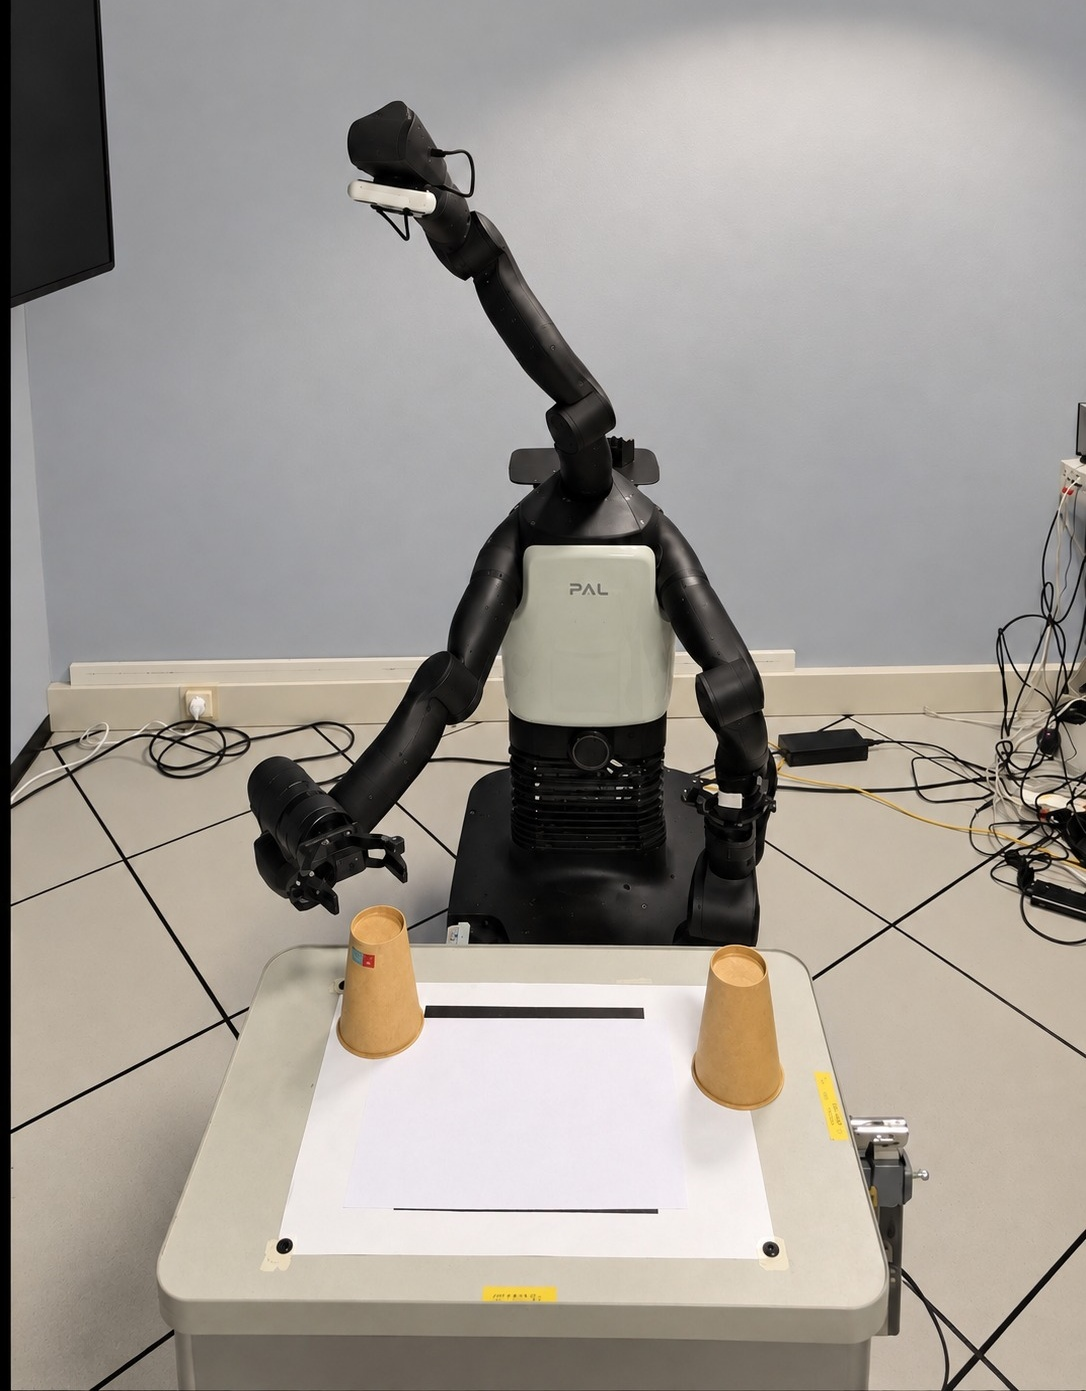
\includegraphics[width=\linewidth]{results/Real_Teleop_10_CFB_SUCCESS/Teleop2_crop.jpeg}\caption{Approaching the near cup}\label{fig:tel-p2}\end{subfigure}
\par\vspace{0.3em}
\begin{subfigure}[t]{0.30\linewidth}\centering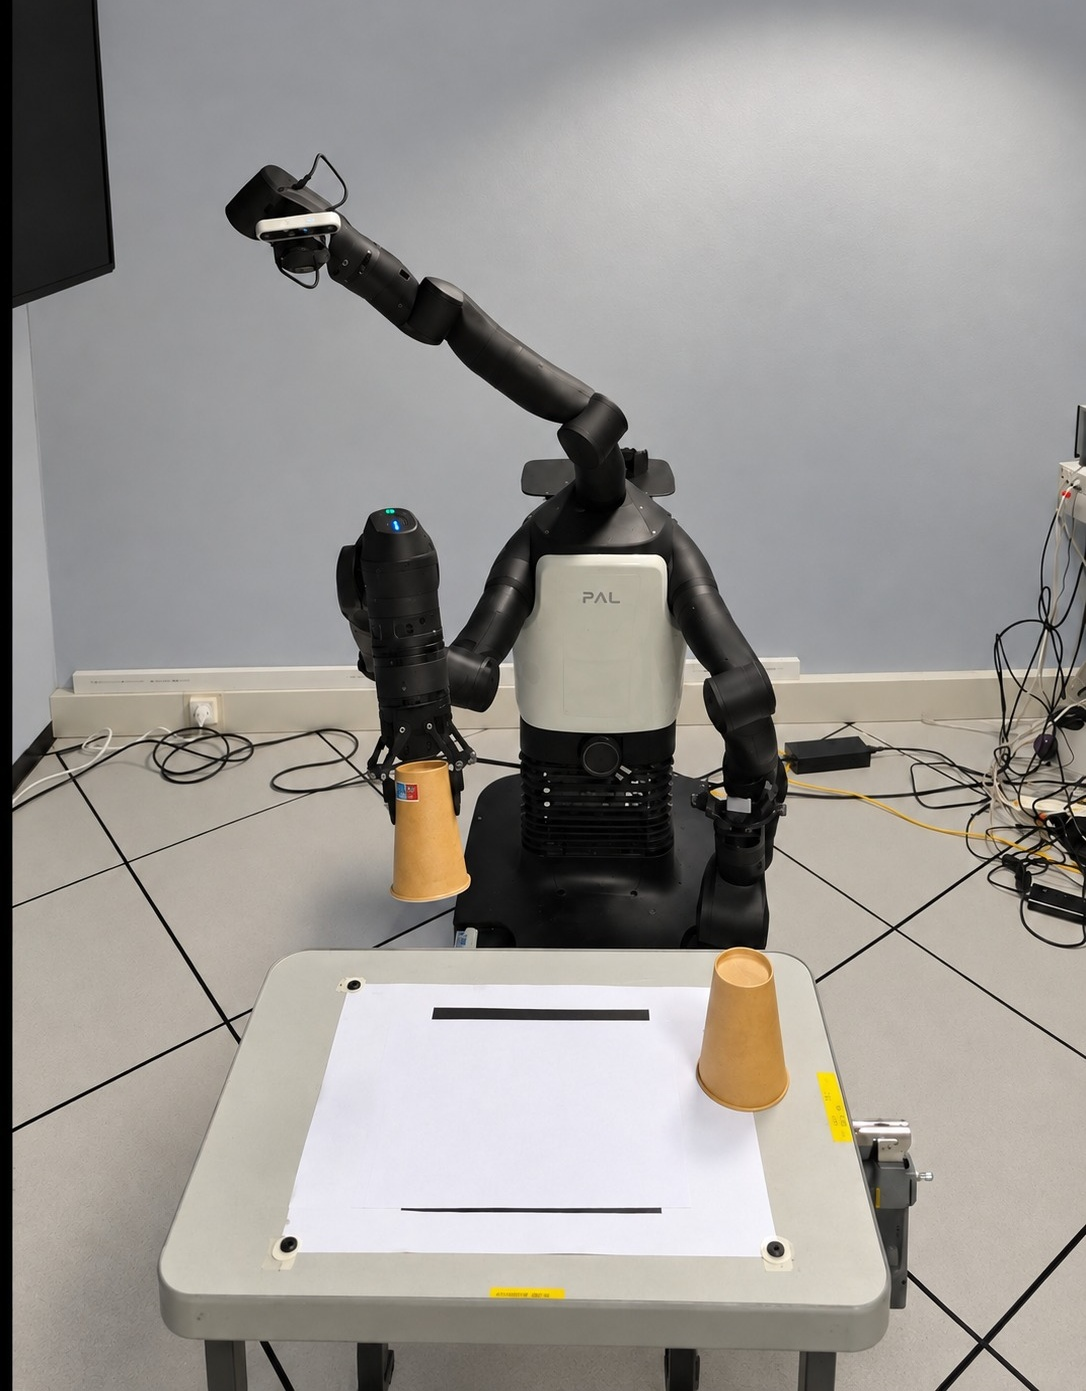
\includegraphics[width=\linewidth]{results/Real_Teleop_10_CFB_SUCCESS/Teleop3_crop.jpeg}\caption{Right cup secured}\label{fig:tel-p3}\end{subfigure}\hspace{1.5em}%
\begin{subfigure}[t]{0.30\linewidth}\centering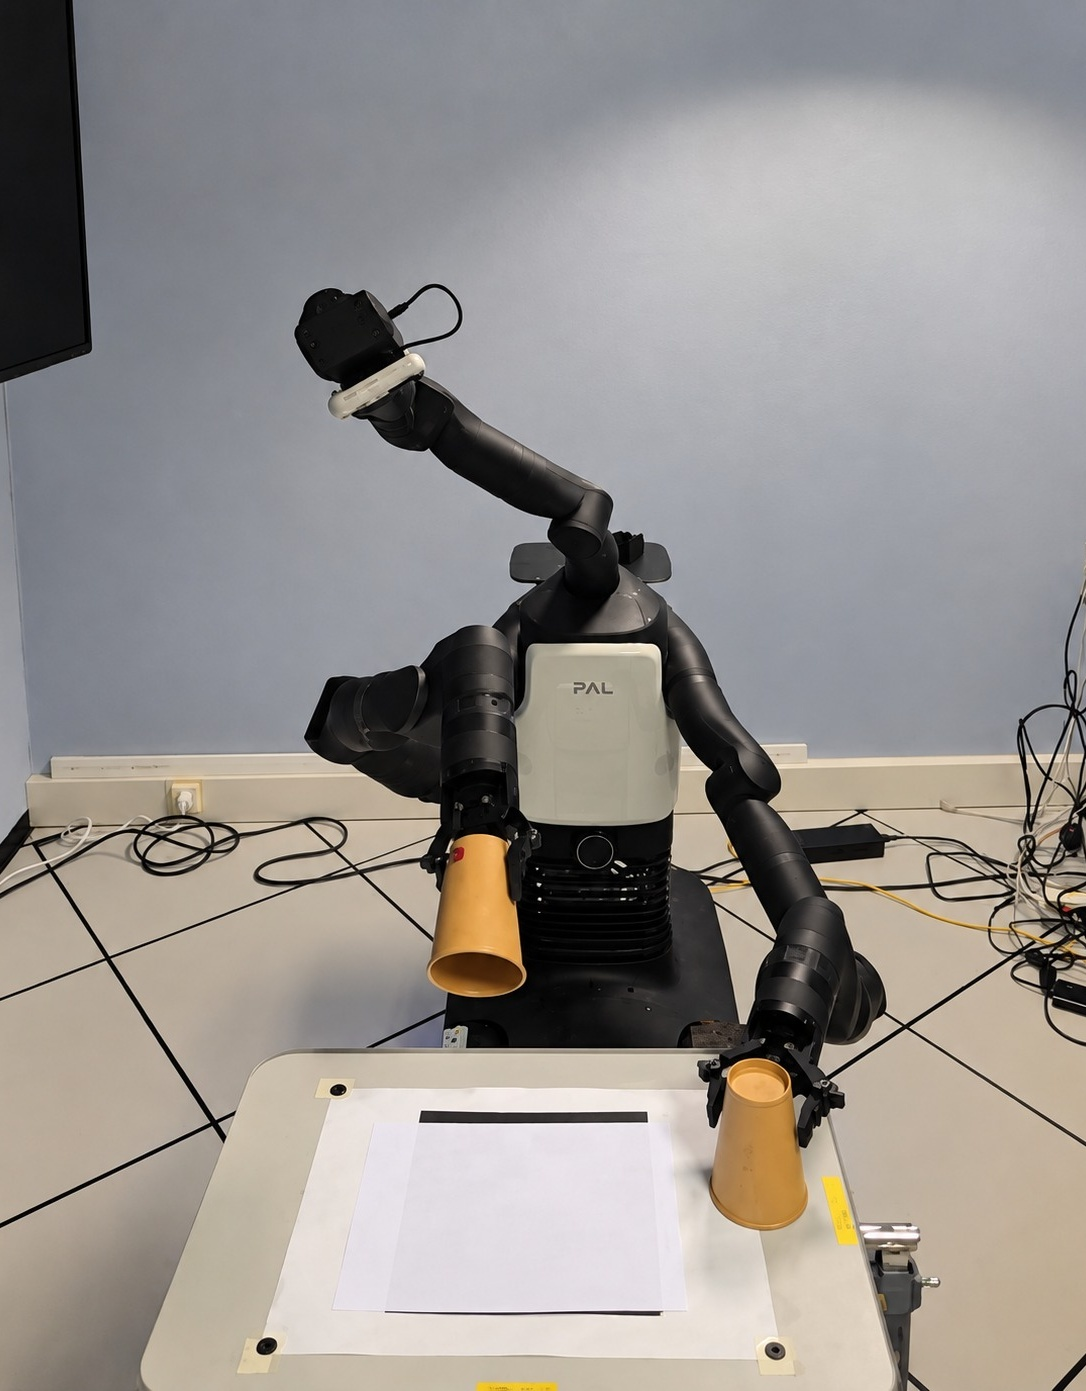
\includegraphics[width=\linewidth]{results/Real_Teleop_10_CFB_SUCCESS/Teleop4_crop.jpeg}\caption{Reaching for the second cup}\label{fig:tel-p4}\end{subfigure}
\caption{The physical trial in sequence: from the home pose, the right arm reaches and secures the first cup, then the left arm engages the second.}
\label{fig:telphotos}
\end{figure}

\textbf{Course of the trial.} Both objects were within reach of either arm; the right arm started active (Figure~\ref{fig:telphotos}). At $t=46.3$~s the operator triggered a grasp on the right cup approached from the side; the state machine held it in alignment for $12.0$~s --- matching the alignment phase's own timeout almost exactly --- without ever issuing a close command, and released it back to the open gripper at $t=58.4$~s: a convergence failure during approach, not a closing or contact failure, since the gripper was never commanded to close at all. The operator repositioned and retried from above at $t=103.2$~s; the gripper closed over $t=109.1$--$111.4$~s and the cup was reported attached at $t=114.4$~s. Control switched to the left arm at $t=132.9$~s, and at $t=171.2$~s the operator triggered a side grasp on the second cup. This attempt was held for $37.8$~s --- longer than either the alignment or the approach phase's own timeout individually --- without a single close command, ending with the gripper explicitly reopened at $t=206.4$~s; the pattern (a long stall at a constant, un-ramped margin, never reaching contact) is the state machine's own signature of a retreat that cannot find clearance, consistent with the wedged or joint-limited case its recovery logic itself checks for. At the trigger, the state machine removed the pair formed by the left gripper and the blue cup from the barrier entirely, rather than relaxing its margin, and held it removed through the stall and the abort retreat that followed; the pair was restored by a fixed $3.0$~s timer at $t=209.4$~s rather than by a measured-clearance test (Section~\ref{sec:grasp}). This revision predates the clearance-gated recovery described there. The controller's own telemetry marks what came next: the CBF shadow price on the left arm, quiet all through the stall, breaks into a ragged, repeatedly re-triggered burst from $t\approx211$ to $217$~s (Figure~\ref{fig:tel-lcbf}) as the arm oscillates against the barrier rather than retreating cleanly, and the operator released the device's deadman switch at $t=217.3$~s, stopping the robot. The recording continues to $253.7$~s, but nothing after the stop reflects the controlled system any longer; every panel below is therefore shown only to $t=230$~s, a few seconds past the stop itself.

\begin{figure}[t]
\hwjointlegend
\begin{subfigure}[t]{0.485\linewidth}\centering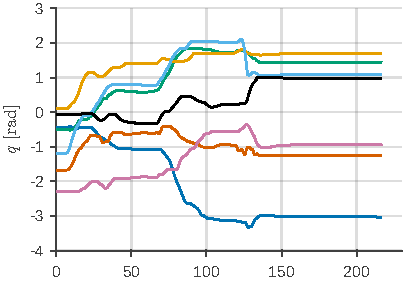
\includegraphics{results/tel_q_R.pdf}\caption{Joint positions, right arm}\label{fig:tel-qR}\end{subfigure}\hfill
\begin{subfigure}[t]{0.485\linewidth}\centering
\includegraphics{results/tel_q_L.pdf}\caption{Joint positions, left arm}\label{fig:tel-qL}\end{subfigure}
\vspace{0.3em}
\begin{subfigure}[t]{0.485\linewidth}\centering
\includegraphics{results/tel_qdot_R.pdf}\caption{Measured joint velocities, right arm}\label{fig:tel-qdR}\end{subfigure}\hfill
\begin{subfigure}[t]{0.485\linewidth}\centering
\includegraphics{results/tel_qdot_L.pdf}\caption{Measured joint velocities, left arm}\label{fig:tel-qdL}\end{subfigure}
\caption{Joint-space view of the teleoperated trial, to $t=230$~s (Section~\ref{sec:hwteleop}).}
\label{fig:telqjoints}
\end{figure}

Figure~\ref{fig:telqjoints} shows the joint-space signature of that same course of events: the right arm moves through the approach and grasp, makes one further, sharp joint-6 adjustment at $t\approx127$~s as the switch pins its weight to the rigid, inactive-arm ceiling, and is essentially static thereafter, while the left arm's joint velocities stay near zero until the switch at $t\approx133$~s and then show two distinct episodes, the grasp approach and, sharply, the $t\approx211$--$217$~s window. There the left arm's velocity trace stops being a single smooth motion and becomes a rapid back-and-forth: joint~4 alone reverses direction roughly every $0.08$~s (about $6$~Hz) at up to $0.11$~rad/s, an order of magnitude faster than any direction change asked of either arm earlier in the trial --- the joint-space trace of the oscillation the shadow price already reports.

\begin{figure}[p]
\hwrllegend
\begin{subfigure}[t]{0.485\linewidth}\centering
\includegraphics{results/tel_lambda_cbf.pdf}\caption{CBF shadow price}\label{fig:tel-lcbf}\end{subfigure}\hfill
\begin{subfigure}[t]{0.485\linewidth}\centering
\includegraphics{results/tel_lambda_jl.pdf}\caption{Joint-limit shadow price}\label{fig:tel-ljl}\end{subfigure}
\vspace{0.4em}
\begin{subfigure}[t]{0.485\linewidth}\centering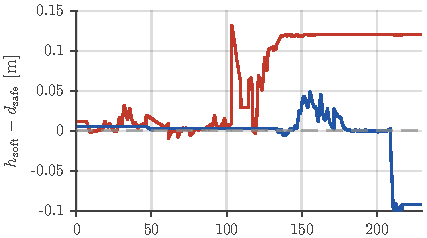
\includegraphics{results/tel_margin.pdf}\caption{CBF safety margin}\label{fig:tel-margin}\end{subfigure}\hfill
\begin{subfigure}[t]{0.485\linewidth}\centering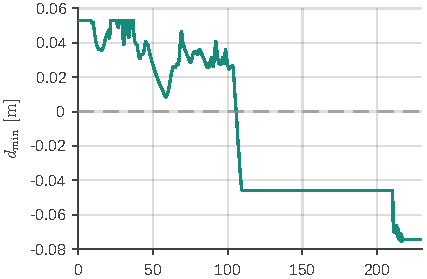
\includegraphics{results/tel_dmin.pdf}\caption{Minimum inter-geometry distance}\label{fig:tel-dmin}\end{subfigure}
\vspace{0.4em}
\begin{subfigure}[t]{0.485\linewidth}\centering
\includegraphics{results/tel_dsafe.pdf}\caption{Velocity-dependent safety margin}\label{fig:tel-dsafe}\end{subfigure}\hfill
\begin{subfigure}[t]{0.485\linewidth}\centering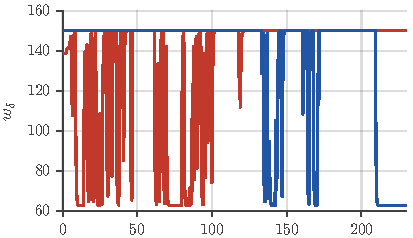
\includegraphics{results/tel_wslack.pdf}\caption{Adaptive slack weight}\label{fig:tel-wslack}\end{subfigure}
\vspace{0.4em}
\begin{subfigure}[t]{0.485\linewidth}\centering
\includegraphics{results/tel_gov_ep.pdf}\caption{Limiter: position error}\label{fig:tel-govep}\end{subfigure}\hfill
\begin{subfigure}[t]{0.485\linewidth}\centering
\includegraphics{results/tel_gov_theta.pdf}\caption{Limiter: orientation error}\label{fig:tel-govtheta}\end{subfigure}
\caption{QP-CLF-CBF and reference-limiter data of the teleoperated trial.}
\label{fig:telqpdata}
\end{figure}

Figure~\ref{fig:tel-lcbf} is the clearest single trace of the trial's three episodes: an early right-arm engagement peaking at $220$ while it first reaches for the near cup ($t\approx9$~s), a left-arm engagement peaking at $172$ once it swings out toward the far one ($t\approx140$~s), and then the $t\approx211$--$217$~s episode, an order of magnitude higher and qualitatively different in shape --- not one spike but a repeatedly re-triggered burst, its single highest sample ($1085$) inside the broken axis's top strip, well above everything else in the trial. The shadow price is exactly zero from the trigger until $t=209.4$~s --- the row does not exist to report anything --- and every recorded solve in the $205$--$218$~s window is feasible, so each command satisfies its own tick's row; yet the margin decreased faster than the discrete counterpart of the nominal barrier condition~\eqref{eq:cbf} on most ticks of the burst, by up to $1.2$~cm per tick, the gap listed in Section~\ref{sec:concllimitations} (candidates include the velocity-dependent margin's unenforced derivative, softmin re-aggregation across pairs, penetration-depth witness normals under deep overlap, up to two ticks of barrier staleness, and the operator's own reference now fighting the row). The joint-limit shadow price of Figure~\ref{fig:tel-ljl} is comparatively quiet --- and, on its own much smaller scale, drawn with the same broken axis as Figure~\ref{fig:tel-lcbf}: a small right-arm burst ($8.5$) as it first leaves the home posture, and one sharp left-arm spike ($27$) at $t\approx140$~s as it swings out toward the far cup, with nothing in the failed-retreat window --- that episode is a collision-barrier event, not a joint-limit one. Figure~\ref{fig:tel-margin} shows the same episode from the constraint side: the left arm's safety margin sits flat near zero for the entire stall because the target pair is off the barrier entirely, then jumps in a single tick from $+2$~mm to $-3.2$~cm at $t=209.4$~s, when the bypass lifts with the gripper already inside the cup's collision envelope, before decreasing further to $-10.0$~cm at $t=214.8$~s. This reading is taken against a constraint re-armed onto an already-violated state, the direct consequence of the pair's deliberate deactivation for the grasp, and is therefore not comparable with the open-loop trial's $-2.6$~mm of Section~\ref{sec:hwswap}, recorded under a continuously enforced row. The right arm's own margin, by contrast, never drops below $-9.5$~mm, reached at $t=61.4$~s as it disengages from the failed first attempt --- a much smaller excursion than the left arm's crisis. Figure~\ref{fig:tel-dmin} carries a second, unrelated negative baseline that is not a safety event at all: raw minimum distance drops to a flat $-4.7$~cm the instant the right cup is attached ($t\approx114$~s) and stays there until the left-arm episode, because the raw metric --- unlike the barrier's own SoftMin margin above, which excludes the carried object --- scores the held cylinder against the gripper envelope it is now resting inside by construction, the same convention documented for the simulated study's clearance metrics. The further drop on top of that baseline, to $-7.5$~cm at $t=216.6$~s, coincident with the left arm's crisis, is consistent with the same left-gripper-and-blue-cup pair now unmasked --- the raw minimum begins moving exactly at $t=209.4$~s --- that is, a model overlap between the left gripper and the blue cup rather than a new contact elsewhere; the pair identity is inferred, since the bag carries no pair-identity telemetry. The velocity-dependent margin of Figure~\ref{fig:tel-dsafe} stays within its configured band throughout, $1.5$--$5.8$~cm, the same $1.5$~cm static floor as Section~\ref{sec:hwswap}; the adaptive slack weight of Figure~\ref{fig:tel-wslack} tracks each arm's own shadow price as designed, collapsing toward its floor whenever that arm's barrier is engaged and recovering toward its ceiling once it is not.

Of the reference limiter's mechanisms, the two shown here are the ones this trial exercises least: the raw and governed traces of both position error (Figure~\ref{fig:tel-govep}) and orientation error (Figure~\ref{fig:tel-govtheta}) coincide throughout for both arms, neither ever approaching the same $0.30$~m and $1.0$~rad ceilings of Section~\ref{sec:hwswap} --- the right arm's own errors, visible from $t=0$ since it alone is referenced from the start, still peak at only $10.2$~cm and $0.74$~rad, both during ordinary teleoperated motion ($t\approx71$ and $127$~s) rather than a clamp. Neither arm's tracking error ever needs governing here because a human operator's own hand motion is already smoother and slower than the quintic reference that trial drives open-loop. The limiter is not idle in this trial, however: it clamps the left arm's commanded linear and angular speed on $6.6\%$ and $11.7\%$ of ticks respectively, concentrated in the same $t\approx211$--$217$~s window --- the operator's own corrective motion during the crisis being what the limiter is actually bounding here, on a channel this figure does not show. Aggregated over the whole trial, the grasp state machine holds authority for $26.7\%$ of ticks, closely matching the $24.1\%$ obtained by summing the three grasp windows above directly from the trigger telemetry.

\begin{figure}[t]
\hwxyzlegend
\begin{subfigure}[t]{0.485\linewidth}\centering
\includegraphics{results/tel_hap_pos.pdf}\caption{Handle position}\label{fig:tel-happos}\end{subfigure}\hfill
\begin{subfigure}[t]{0.485\linewidth}\centering
\includegraphics{results/tel_hap_rpy.pdf}\caption{Handle orientation (roll, pitch, yaw)}\label{fig:tel-haprpy}\end{subfigure}
\vspace{0.4em}
\begin{subfigure}[t]{0.485\linewidth}\centering
\includegraphics{results/tel_hap_vlin.pdf}\caption{Handle linear speed}\label{fig:tel-hapvlin}\end{subfigure}\hfill
\begin{subfigure}[t]{0.485\linewidth}\centering
\includegraphics{results/tel_hap_vang.pdf}\caption{Handle angular speed}\label{fig:tel-hapvang}\end{subfigure}
\vspace{0.4em}
\begin{subfigure}[t]{0.485\linewidth}\centering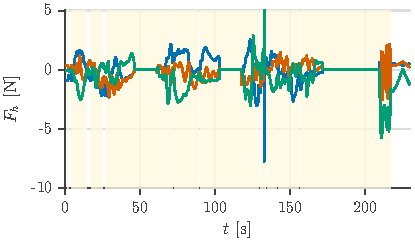
\includegraphics{results/tel_hap_force.pdf}\caption{Force rendered on the handle}\label{fig:tel-hapforce}\end{subfigure}\hfill
\begin{subfigure}[t]{0.485\linewidth}\centering
\includegraphics{results/tel_hap_torque.pdf}\caption{Torque rendered on the handle}\label{fig:tel-haptorque}\end{subfigure}
\caption{Haptic-device telemetry of the teleoperated trial, in the device base frame.}
\label{fig:telhaption}
\end{figure}

\textbf{Operator side.} Figure~\ref{fig:telhaption} is the same trial seen from the handle. The shaded windows are those in which the operator is in control --- deadman held and clutch released --- $87\%$ of the shown span; the white gaps are clutch holds, in which the handle is re-indexed without moving the reference (Section~\ref{sec:clutchmode}). The gaps are where the handle moves fastest: every angular-speed peak above $2$~rad/s, up to $4.1$~rad/s, falls inside one (Figure~\ref{fig:tel-hapvang}), against $2.0$~rad/s at most while in control, and the same holds for linear speed ($0.56$ against $0.36$~m/s) --- the operator's re-orientation of their own wrist between indexing strokes, never a command to the robot. The rendered force (Figure~\ref{fig:tel-hapforce}) stays within a few newtons for the whole trial, touching the $10$~N clip of the force manager exactly once, at the arm switch ($t=132.9$~s), when the tether re-anchors from the right arm's pose to the left's in a single tick. Torque (Figure~\ref{fig:tel-haptorque}) stays inside its $1$~N\,m clip (peak $0.92$); the three dense bands are not operator load at all but the vibrotactile cue rendered whenever the grasp state machine holds authority, and they coincide exactly with the three grasp windows above --- during those, no other force is impressed on the handle.

\begin{figure}[t]
\centering
\begin{subfigure}[t]{0.485\linewidth}\centering
\includegraphics{results/tel_sa_alpha.pdf}\caption{Blending authority}\label{fig:tel-saalpha}\end{subfigure}\hfill
\begin{subfigure}[t]{0.485\linewidth}\centering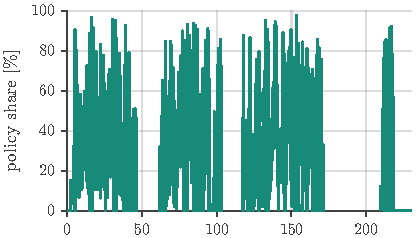
\includegraphics{results/tel_sa_share.pdf}\caption{Policy share of the blended action}\label{fig:tel-sashare}\end{subfigure}
\vspace{0.4em}
\begin{subfigure}[t]{0.485\linewidth}\centering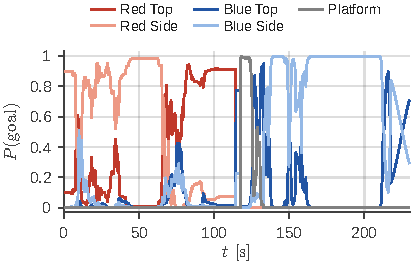
\includegraphics{results/tel_sa_belief.pdf}\caption{Goal belief}\label{fig:tel-sabelief}\end{subfigure}\hfill
\begin{subfigure}[t]{0.485\linewidth}\centering
\includegraphics{results/tel_sa_state.pdf}\caption{Active arm and autonomous grasp}\label{fig:tel-sastate}\end{subfigure}
\caption{Shared-autonomy telemetry of the teleoperated trial.}
\label{fig:telsa}
\end{figure}

\textbf{Shared autonomy.} Figure~\ref{fig:telsa} is the arbitration layer's own account. The blending authority $\alpha$ of~\eqref{eq:blend} (Figure~\ref{fig:tel-saalpha}) drops to exactly zero throughout each grasp window, where the state machine rather than the blend owns the reference; excluding that $26.5\%$ of the trial, it is non-zero on $63\%$ of the remaining ticks, never crosses $0.73$, and averages $0.17$ --- the policy is always the minority partner. The share panel (Figure~\ref{fig:tel-sashare}) restates this in the action itself, $\alpha\|v_{\text{policy}}\|$ as a fraction of the blended twist's two contributions --- the user's share is its complement, and is not drawn --- with a median of $36\%$ where the blend is active. The belief (Figure~\ref{fig:tel-sabelief}) tracks the operator's intent through the trial's four decisions: red-side dominates the first approach, red-top takes over cleanly once the operator re-approaches from above ($t\approx100$~s), the platform goal briefly wins ($t\approx117$--$133$~s) as the operator, cup in hand, moves toward the placement station before switching arms instead, and blue-side rises to $0.998$ once the left arm is driven. Its only sustained ambiguity is blue-top against blue-side while the left arm is still far from the cup, resolved as the approach commits. Figure~\ref{fig:tel-sastate} is the discrete state under all of it: the active arm and the three windows in which a grasp, not the operator, is driving.

\section{Setup of the user study}
\label{sec:study}

The system is the apparatus of a user study run in a matched simulation environment; Section~\ref{sec:hwvalidation} reports the separate validation of the same controller and its perception pipeline on the physical robot. The design is a $2\times3$ matrix crossing the teleoperation mapping with the assistance strategy:
\begin{itemize}[nosep]
\item \textbf{Control mode}, two levels --- \textsc{clutch}, position control with indexing (Section~\ref{sec:clutchmode}), and \textsc{joystick}, spring-centred velocity control (Section~\ref{sec:joystick});
\item \textbf{Assistance strategy}, three levels --- \emph{F}, the guidance force~\eqref{eq:fguide} rendered on the handle; \emph{B}, reference-level arbitration~\eqref{eq:blend} of the user twist with the belief-weighted policy; and \emph{FB}, both together.
\end{itemize}
This yields six conditions (Table~\ref{tab:cells}). The two channels are orthogonal by construction: F acts only on the handle and never modifies the reference; B acts only on the reference and is never rendered on the handle. Consequently the combined level is the exact superposition of the two single-channel levels --- the guidance wrench under FB is identical to the one under F, and adding B changes only \emph{which} reference the base tether tracks, not the rendered assistance law. Each control mode is also implemented with neither channel active, so the system realises eight configurations in all; the two unassisted ones are used for familiarisation and as a reference trace, and are excluded from the study matrix. The two unassisted configurations are not part of the study matrix, so the study compares assistance strategies with one another and the two mappings with one another; it makes no claim that assistance outperforms unassisted teleoperation, which would require an internal baseline that this design does not run, and results reported elsewhere on other tasks cannot substitute for it. With three assistance levels (F, B, and FB) rather than the full $2\times2$ of the two channels, the independent effect of each channel and their interaction are not separately estimable: F versus FB isolates adding blending to guidance, and B versus FB isolates adding guidance to blending, and that is the extent of the channel design. The question this design does ask --- which channel, under which mapping, and how the two combine --- is not answered by that literature, so every one of the six conditions contributes to it.

\begin{table}[b]
\centering\footnotesize
\begin{tabularx}{\textwidth}{@{}lcccLL@{}}
\toprule
Condition & Code & F & B & Operator feels & Arm reference written by \\
\midrule
\textsc{clutch} guided feedback  & CF  & \checkmark & --     & tether $+$ guidance bias & teleop \\
\textsc{clutch} guided blending  & CB  & --     & \checkmark & tether (blended reference) & blending layer \\
\textsc{clutch} full guidance    & CFB & \checkmark & \checkmark & tether $+$ guidance bias & blending layer \\
\addlinespace[2pt]
\textsc{joystick} guided feedback & JF  & \checkmark & --     & spring $+$ guidance bias & teleop \\
\textsc{joystick} guided blending & JB  & --     & \checkmark & spring & blending layer \\
\textsc{joystick} full guidance   & JFB & \checkmark & \checkmark & spring $+$ guidance bias & blending layer \\
\bottomrule
\end{tabularx}
\caption{The six study conditions ($2$ control modes $\times$ $3$ assistance strategies). The code names each condition by its control mode, C for \textsc{clutch} and J for \textsc{joystick}, followed by its active assistance channels, and is the label used on every results figure. The guidance bias is~\eqref{eq:fguide}; the blending layer is the arbitration of Section~\ref{sec:blend}.}
\label{tab:cells}
\end{table}

Every condition shares Chapter~\ref{ch:method}'s architecture --- safety controller, belief estimation, goal manifolds, grasp state machine, and every shared building block (homing, damping, vibrotactile cues, authority cap) --- byte-identical throughout; only the operator-input mapping and the rendered assistance change, so a measured difference between two conditions is attributable to those factors alone.

Two asymmetries remain by design and are declared rather than equalised: the joystick base force is a \emph{homing} spring while the clutch base force is an \emph{error-tracking} tether, since each mapping mandates its own base feedback (Section~\ref{sec:columnbase}); and the guidance saturation is absolute in the clutch mapping but deadzone-exit-calibrated in the joystick mapping~\eqref{eq:kappacal}, to stay commensurate with that base-force landscape.

\subsection{Task and workspace}
\label{sec:studyworld}

Each participant works through two scenarios under every assigned condition. The two are chosen to differ in one structural respect --- whether the task \emph{requires} the arms to cooperate --- while keeping the object set, the grasp vocabulary, and the delivery-to-a-station goal common to both. This scenario factor is crossed with, and orthogonal to, the assistance factorial of Table~\ref{tab:cells}: assistance that helps a single arm run its own errand need not be the assistance that helps two arms hand an object between them.

\textbf{Relay scenario.} The task is a bimanual relay. Two industrial batteries --- modelled as plain cylinders for collision purposes --- rest on a table in front of the robot, and both must be delivered to a single station on a conveyor unit standing to the robot's right. A storage-rack shelf spans the table just above the batteries, closing the overhead approach corridor and forcing every pick and every place at the table to be a side grasp. The conveyor sits clear of the shelf, so its station admits a top approach, but only the right arm reaches it. The right arm can therefore pick its battery and carry it straight to the conveyor; the left arm cannot, and instead stages its battery on an intermediate handover disk on the table --- offset toward the robot's right so that it falls within both arms' reach --- from which the right arm relays it onward.

The handover is forced by workspace geometry alone, not by an inserted divider: only the right arm reaches the delivery station, so a run that never hands over cannot finish. Both scenes also carry decorative fixtures --- fencing, a gantry, cabinets, pallets, conveyor frames --- that give visual context but declare no collision geometry; each scenario's declared model is limited to the table, the two batteries, its own blocking structure, and one convex envelope per conveyor.

\begin{figure}[t]
\centering
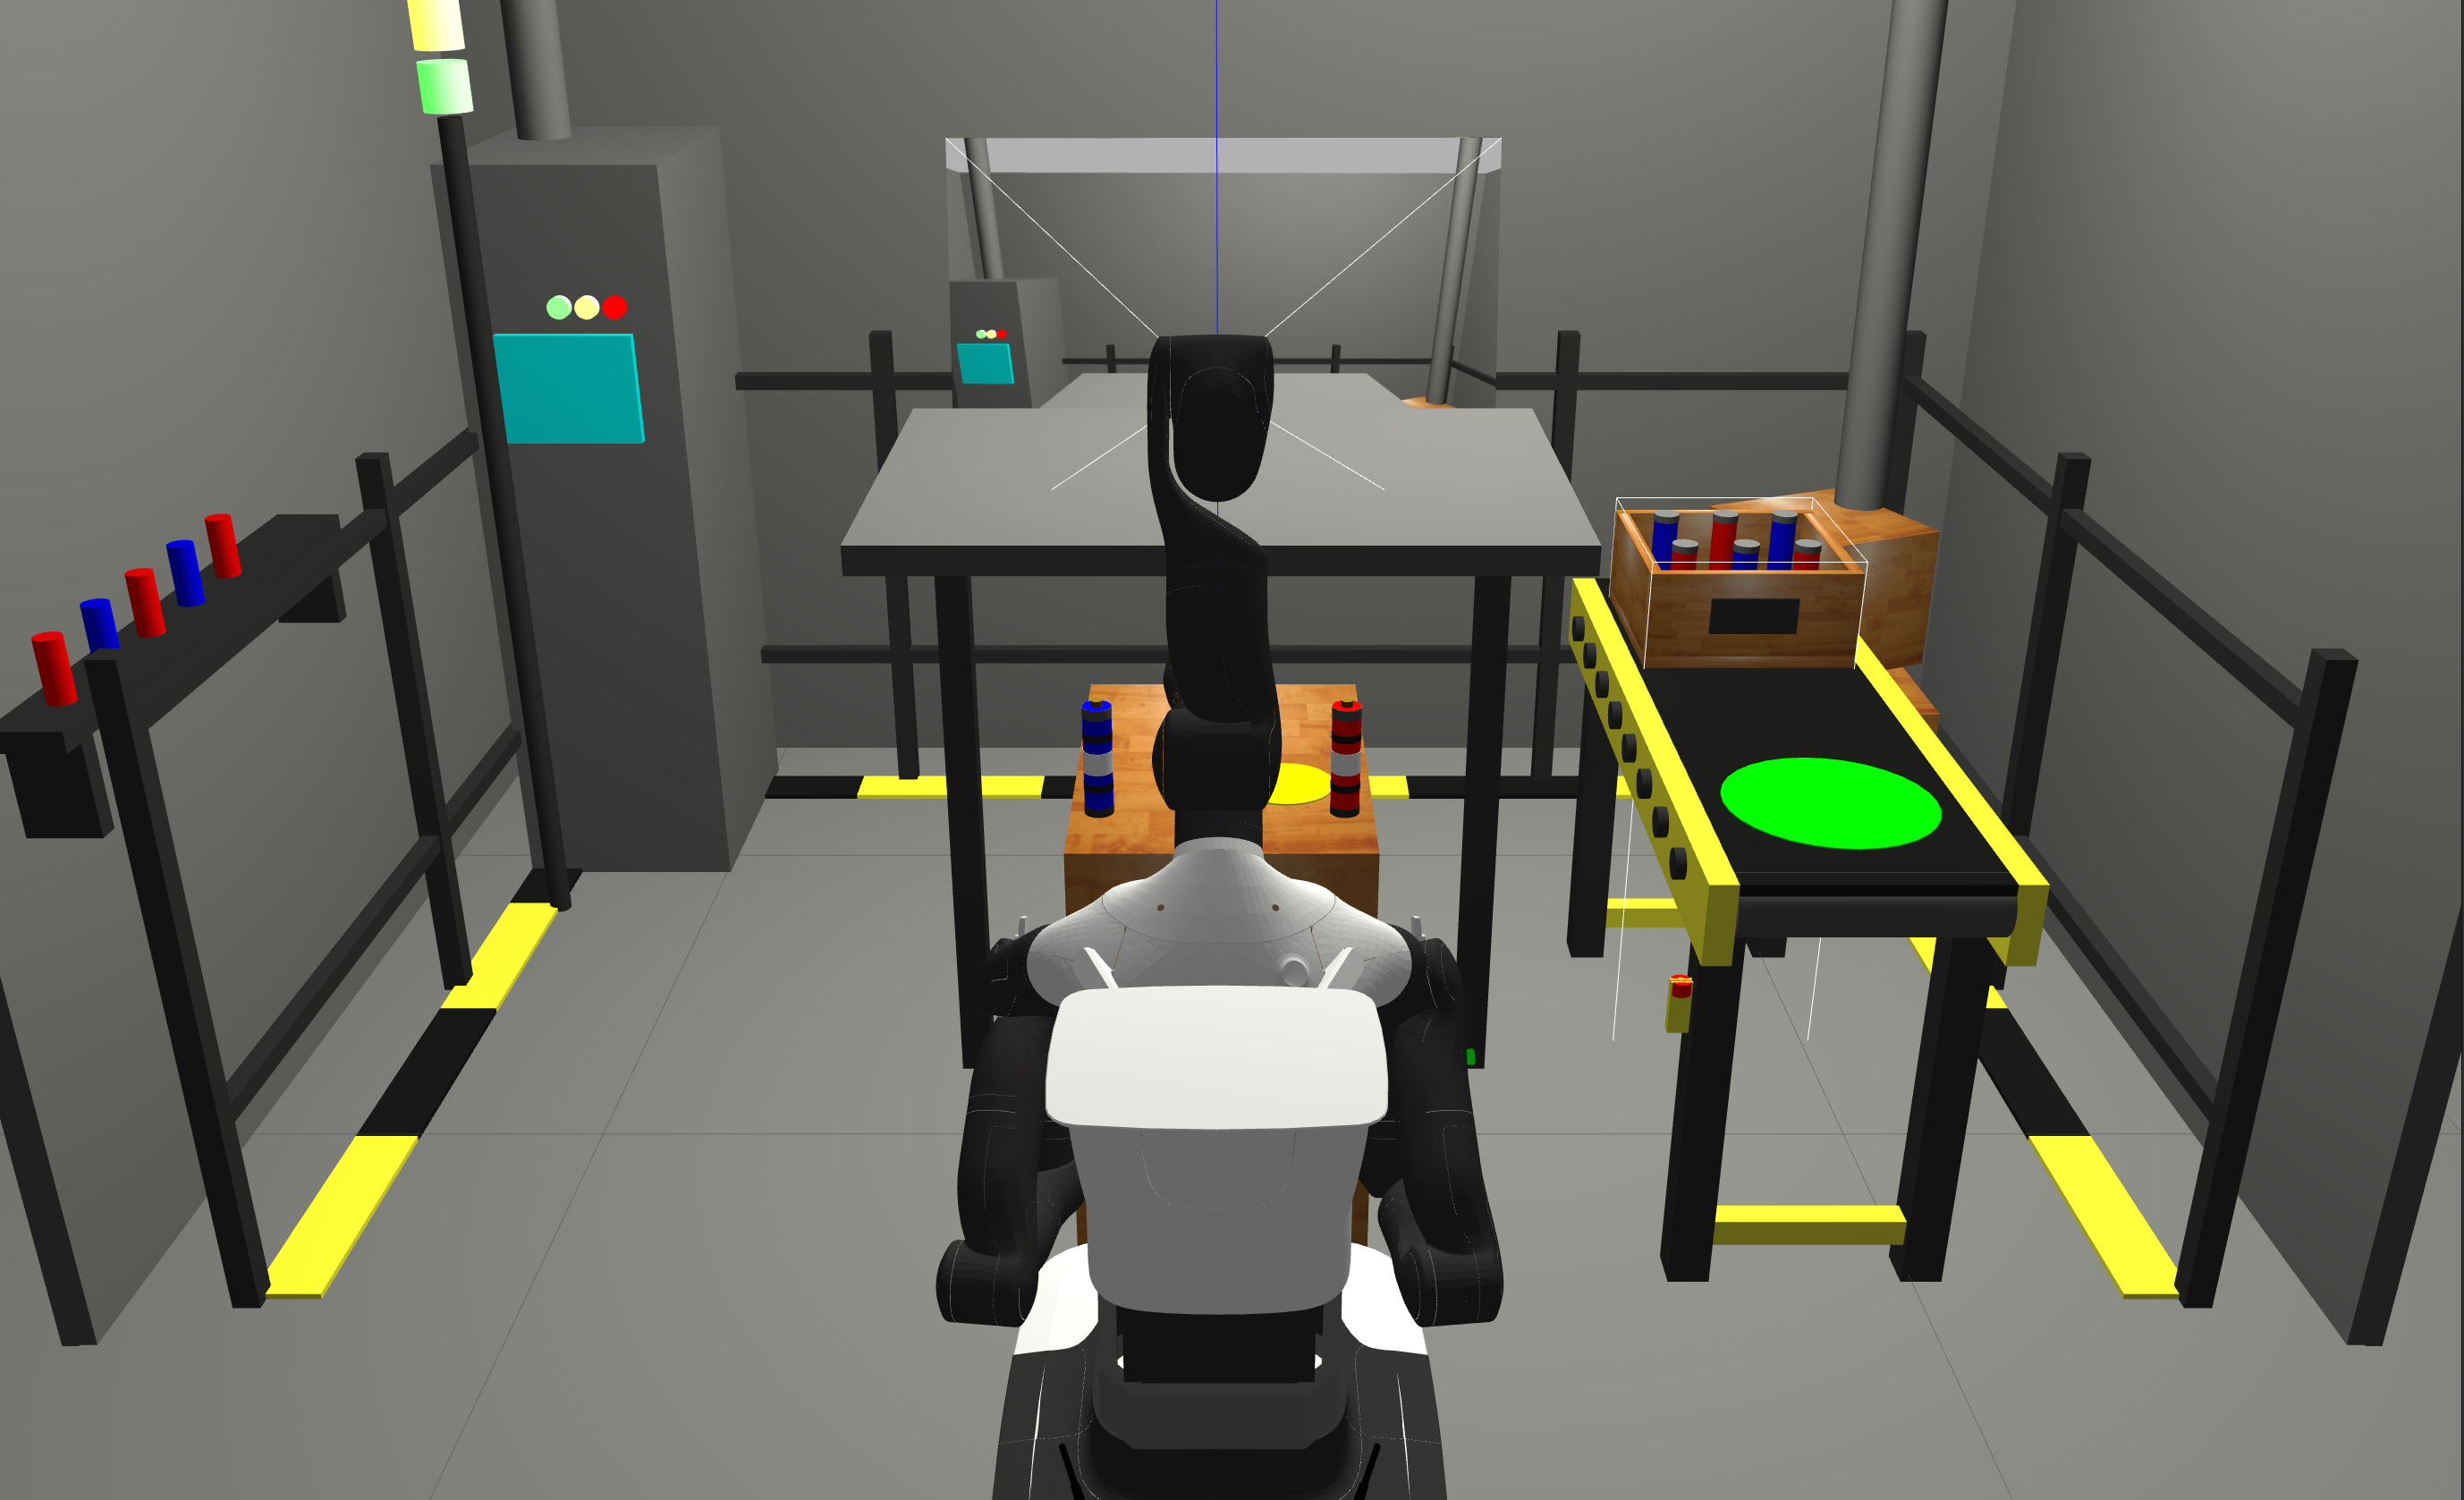
\includegraphics[width=0.85\linewidth]{rackworld.png}
\caption{The relay scenario, from behind the robot: the rack shelf forces a side grasp, relayed via the handover disk (yellow) to the right arm.}
\label{fig:rackworld}
\end{figure}

\textbf{Independent scenario.} The task is two independent, concurrent pick-and-place errands, one per arm. A thin safety shield stands between the robot and the table, spanning its full width so that no lateral window is left; each arm must therefore reach \emph{over} the shield to work. Two conveyor units flank the table, mirror-symmetric about the robot's sagittal plane, each carrying its own delivery station. Each arm picks the battery on its own side and delivers it to the station on that side: the errands are symmetric, with no handover and nothing contested between the arms. Because the shield closes the low approach and leaves the overhead corridor open, every grasp here is a top grasp --- the complement of the relay scenario, where the shelf closes the overhead corridor and every grasp is a side grasp. Between them the two scenarios exercise both grasp manifolds of Section~\ref{sec:policies} and both the coordinated and the independent regimes of the bimanual controller.

Each scenario declares its placement stations as platforms --- the handover disk and the conveyor station in the relay scenario, the two mirrored conveyor stations in the independent one. Each is demandable by either arm while that arm holds a battery, and belief estimation together with guidance selects which platform is the active placement goal, exactly as they select among grasp goals (Section~\ref{sec:policies}). Like every platform, they are reference poses for the goal manifold and the guidance law alone, and none enters the collision model.

Both scenarios exercise the whole architecture, not just the driven arm. The relay's handover is a bimanual case of Section~\ref{sec:locality}'s single-arm gap: no per-arm policy decides which arm carries the battery or when to hand off, so the operator does. The head faces the same test: tracking the gripper's top-grasp approach axis (Section~\ref{sec:headtrack}) forces it above the shield's full-height collision box, a viewpoint the relay scenario never demands. Belief estimation is stressed alike: every battery carries a top and a side goal candidate regardless of which the geometry admits (Section~\ref{sec:policies}), so the belief sum~\eqref{eq:objbelief} must resolve the intended approach from poses that start close together.

\subsection{Environment model and camera use}
\label{sec:studyenv}

Two facts about the environment fix what the study tests. First, the collision world in every study trial is the declared model of Section~\ref{sec:task}, loaded from the scenario's description file; the autonomous perception pipeline of Section~\ref{sec:convergence} is not in the loop, so no trial's safety depends on the camera's estimate of the scene. Second, the head is nonetheless active throughout, running the active-arm visual servoing of Section~\ref{sec:headtrack} to keep its camera trained on the gripper being driven. That camera image is shown alongside the operator's RViz views of the session; the two are not interchangeable. The RViz views are what actually render the reference the operator is assumed throughout this thesis to be watching~(Section~\ref{sec:blend}), since a raw camera image carries no such marker. That marker is also the operator's only cue to the blending channel: it is orange while the operator's own input still dominates the blended reference, and turns green once the belief-weighted policy visibly takes over, tracking the same authority $\alpha$ of~\eqref{eq:blend} that drives the reference itself. Guidance and blending are thus felt through different senses --- the guidance bias of Section~\ref{sec:guidance} as a force on the handle, blending as a color the operator watches --- consistent with the two channels never sharing an output (Section~\ref{sec:study}). The camera image supplements this with close visual detail on the gripper itself; it serves the operator's perception, not the controller's, but it is not where the reference is seen.

\begin{figure}[t]
\centering
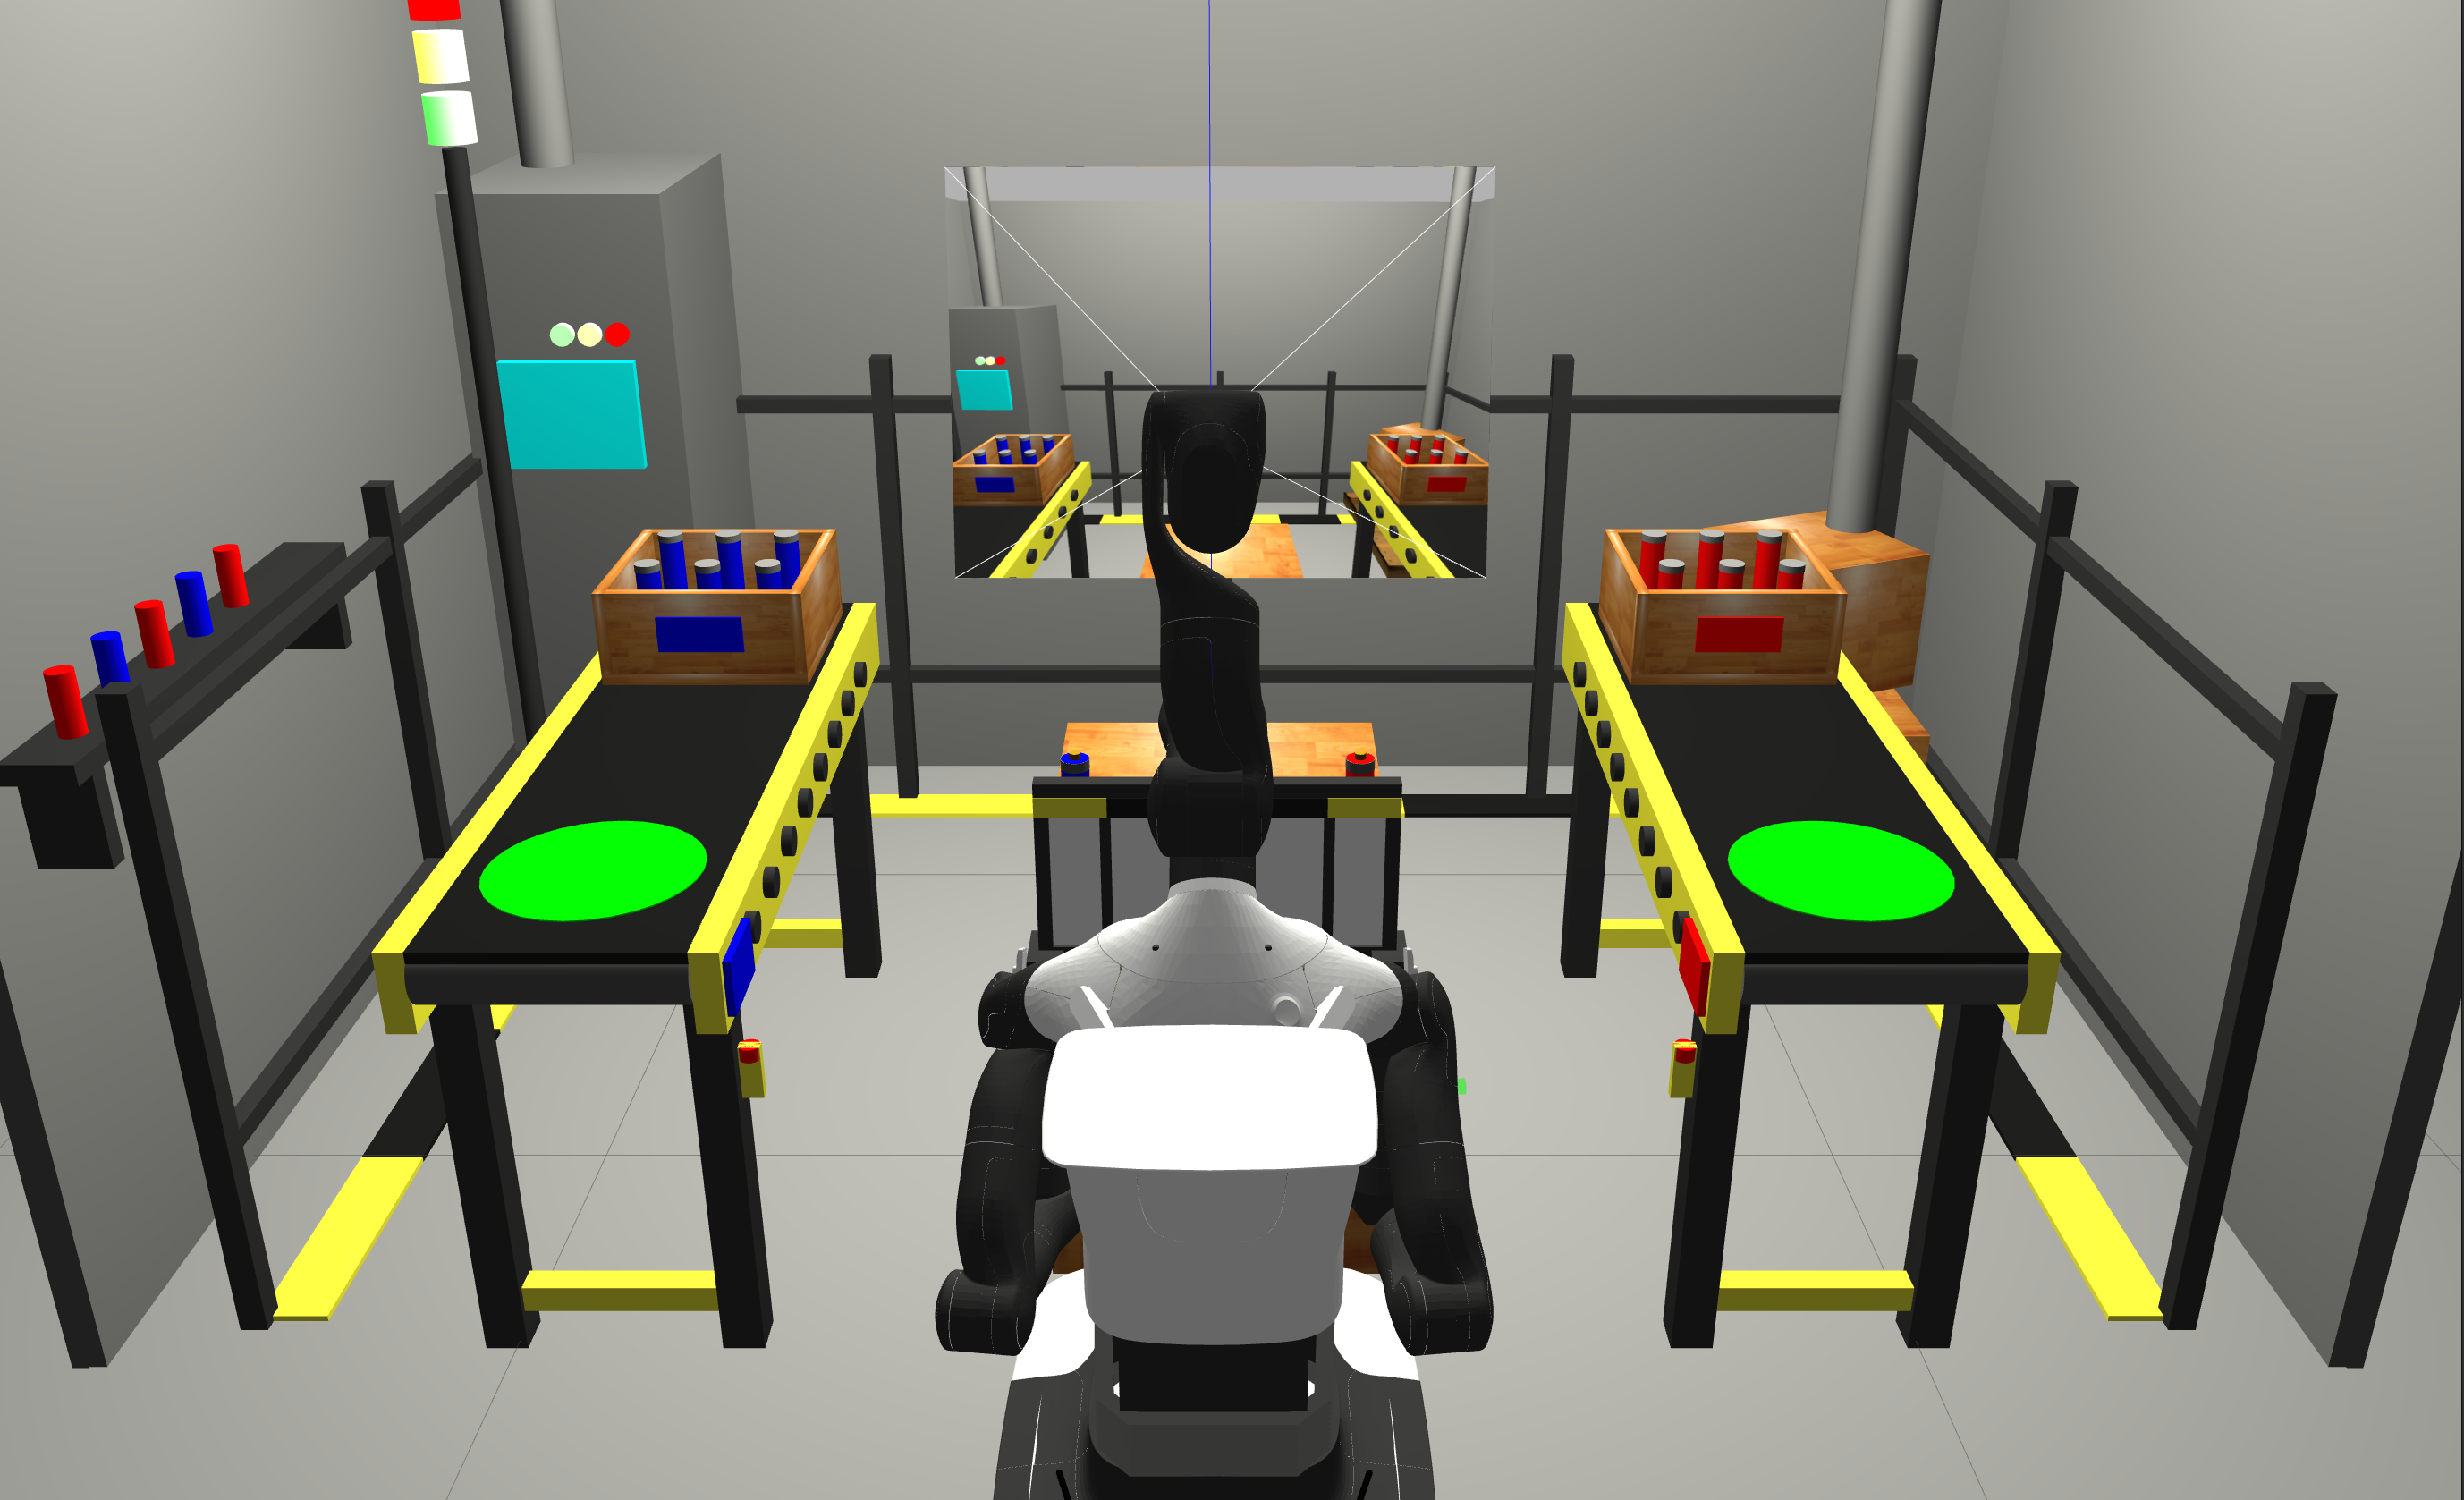
\includegraphics[width=0.85\linewidth]{shieldworld.png}
\caption{The independent scenario, from behind the robot: the shield forces a top grasp; each arm serves its own mirrored conveyor, independently.}
\label{fig:shieldworld}
\end{figure}

\subsection{Apparatus and instrumentation}
\label{sec:studyapparatus}

All sessions run on a single workstation --- Ubuntu 22.04 LTS, ROS~2 Humble, Gazebo Classic 11.10.2, an Intel Core i9-14900HX CPU, and an NVIDIA RTX 4090 Laptop GPU driving the Gazebo and RViz rendering. A single bringup starts the simulator and the robot model, the robot's default arm and torso controllers, the mobile-base teleoperation, and five simultaneous views of the task (Figure~\ref{fig:studyviews}). A Gazebo view from behind the robot shows the whole scene --- what an operator positioned behind the physical robot would see --- and the robot's own head camera, servoed to the driven gripper (Section~\ref{sec:headtrack}), gives a close, zoomed view of it. Three RViz views complete the operator's picture: one static view framed on the table where the batteries sit, and two views that each track one gripper, so the reference stays within at least one view's field of view whichever arm is active. All three RViz views share the Gazebo view's rear-facing azimuth --- no side or top perspective is offered --- since the device-to-robot frame convention (Section~\ref{sec:device}) is itself defined for an operator positioned behind the robot, and a perspective inconsistent with it risks disorienting a first-time participant. Each RViz view renders a filtered robot description in which every link outside the two arm-and-gripper chains is dimmed to a translucent grey, so that the operator's sight line to the hands and the task is not blocked by the robot's own torso, base, and head. The filter acts at the description source --- it rewrites the model the visualiser loads --- because per-link transparency overrides applied inside the visualiser have no visual effect on this robot's meshes. Collision and inertial data are left untouched, and the unfiltered description stays available to every other consumer.

\begin{figure}[t]
\centering
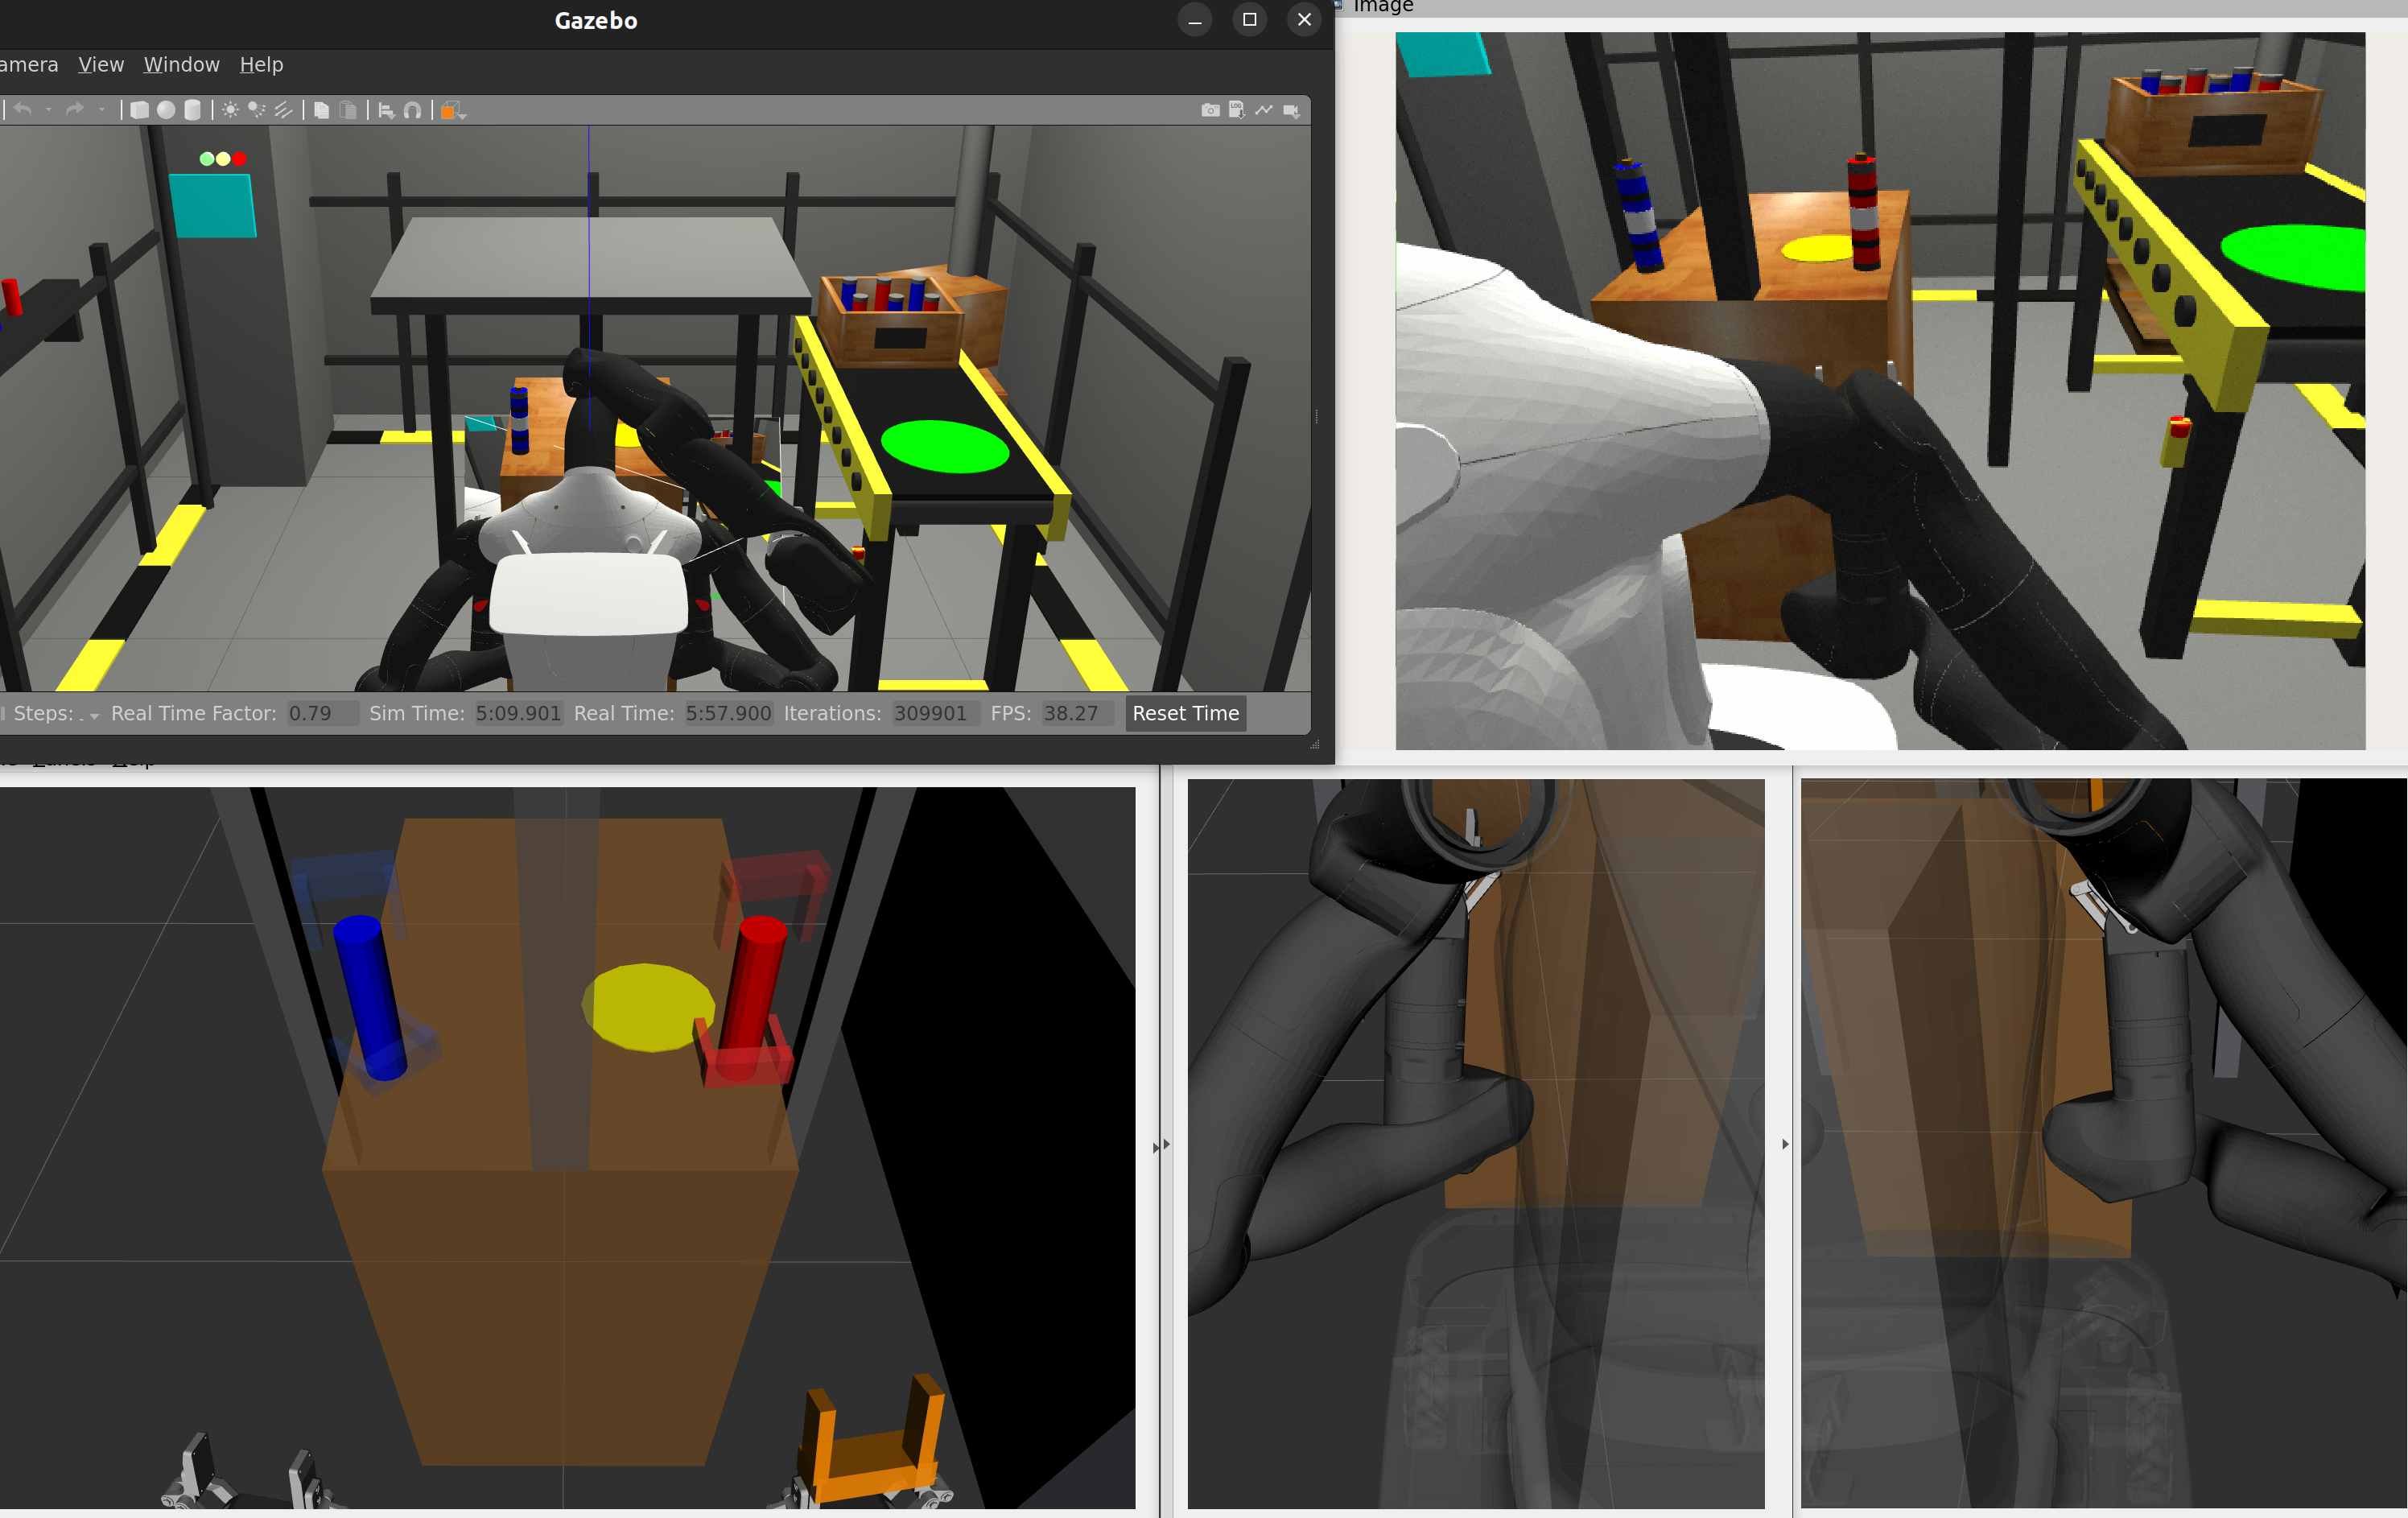
\includegraphics[width=0.85\linewidth]{generalview.png}
\caption{The general view of the operator's picture during a session.}
\label{fig:studyviews}
\end{figure}

\textbf{Operator controls.} The operator issues every discrete command through the handle's buttons, as described in Section~\ref{sec:opcontrols}. The alignment torque rendered while the clutch is held~\eqref{eq:aligntorque} is not captured by the study's translational effort measure, which is defined on the rendered force alone. The arm left inactive by a switch, and one currently executing an autonomous grasp, both bypass the adaptive slack schedule (Section~\ref{sec:sched}): their weight is pinned at the ceiling instead, so the inactive arm's hold is rigid and the grasping arm's alignment converges inside tolerance.

\textbf{Startup homing.}
\label{sec:homing}
Every session opens with a homing phase in which the only rendered wrench is a soft parking spring of the form of~\eqref{eq:fhome}, drawing the handle to a fixed neutral pose and faded in over a fixed interval, so that every participant begins from the same handle configuration; the spring is far softer than either mapping's operating spring, since the operator need not be holding the handle while it runs. The phase ends once the handle has held within position and orientation tolerances for a settle window, or after a timeout.

\subsection{Procedure}
\label{sec:studyprocedure}

Each session opens with a briefing in which the operating principles of the platform, the two control modes, and the assistance strategies the participant encounters are explained in detail. The interaction is framed explicitly as cooperative: participants are told to read the robot's guidance, whether the haptic bias or the blended reference, as collaborative assistance correcting them toward the intended goal rather than as an antagonistic force to resist, and are encouraged to work with each assistance channel rather than against it.

The briefing is followed by an unassisted familiarisation phase in a custom, simplified scene containing only the two target batteries on a bare tabletop, with every obstacle removed and neither assistance channel active. Within this scene, participants operate the haptic device with both the clutch and the joystick mapping (Sections~\ref{sec:clutchmode} and~\ref{sec:joystick}), for as long as they judge necessary. The phase serves two purposes: it lets the operator acclimatise to the device's baseline dynamics, kinematic mapping, and passive forces before either assistance channel is introduced, and it lets the operator complete the reaching task once unassisted, establishing a personal baseline against which the assistance strategies met in the formal trials can be judged. No data are recorded during familiarisation.

No individual trial carries a completion threshold or a time limit. Because a participant's data enter the analysis only as a complete six-condition record, discarding any single trial would discard the entire session rather than one data point, so nothing is gained by rushing a trial and every participant is given as long as the task requires. A complete session, from the opening briefing to the closing questionnaire, takes approximately one hour.

The six formal conditions are then run in an order fixed by a balanced Latin square, a Williams design: within each control mode, the three assistance levels are sequenced in one of the six possible orders, so that every level is preceded by every other level an equal number of times across the design, and the two three-condition blocks are further ordered so that the leading mode is balanced across participants, a balance the learning-effect analysis of the results draws on. Because three conditions admit only six distinct orderings in total, the minimal design that balances immediate order effects coincides here with the complete permutation set; crossed with the two possible leading modes it yields twelve distinct sequences, each realised by two of the twenty-four participants.

\section{Results}
\label{sec:results}

Twenty-four participants complete the full grid of six conditions on both scenarios, giving 288 analysed trials; the count follows the design, not convenience, since the schedule realises twelve counterbalanced orderings of the six conditions, each run by two participants. Every quantity below is first reduced to one number per trial, then averaged over the two scenarios so that each participant contributes exactly one value per condition, and it is those participant-level values that enter every test and every figure.

\subsection{Statistical procedure}
\label{sec:stats}

The design is fully within-subject with two factors, the control mode --- clutch or joystick --- and the assistance channel --- force guidance alone, reference blending alone, or both. Each measure is therefore examined with a two-way repeated-measures analysis of variance over mode and assistance, and, because the six conditions are also of interest individually, with a Friedman test over the six cells followed by pairwise Wilcoxon signed-rank tests whose $p$ values are corrected with the Holm step-down procedure inside each metric family. The significance level is $0.05$ throughout.

Two assumptions govern which of those two tracks carries a claim. Normality is assessed with the Shapiro--Wilk test applied to the residuals of the two-way model, $y_{pc} - \bar y_{p\cdot} - \bar y_{\cdot c} + \bar y$ with $p$ the participant and $c$ the condition, one test per measure, and to the within-participant paired differences that feed the Holm-corrected Wilcoxon tests, rather than to each condition in isolation; sphericity is assessed with Mauchly's test on the assistance factor; where sphericity is rejected, the Greenhouse--Geisser correction is applied to the degrees of freedom and the corrected $p$ value is the one reported. Sphericity is not testable, and is assumed, for a factor with only two levels, which covers the mode factor everywhere and the assistance factor in the intent-estimation and shared-authority measures that exist only where blending is active, since those are compared over the two blended assistance levels alone. Table~\ref{tab:assumptions} collects both checks together with the outcome of the three analysis-of-variance effects.

The picture that table paints is the reason the non-parametric track is treated as primary here. Residual normality fails for seven of the fourteen measures ($L$, $\bar\Phi$, $\bar\delta$, $h_{\min}$, $T_\lambda$, $\rho$, and $\Delta_{\max}$), and four fail Mauchly on the assistance factor ($L$, $\bar\delta$, $h_{\min}$, and $\bar f$ under the clutch mapping). Minimum clearance is the extreme case on both counts, for a reason that is structural rather than statistical: the barrier itself pins the measure near a fixed floor, a structural explanation the safety results take up in more detail. Consequently, the analysis of variance is reported for the structure it reveals --- whether an effect lives in the mode, in the assistance, or in their interaction, and how much variance it explains --- while every claim that one condition differs from another rests on the Holm-corrected rank tests drawn on the figures. As a check on that division of labour, a fully non-parametric factorial analysis, the aligned rank transform~\cite{wobbrock2011art}, is run on all thirty-nine tested effects; it agrees with the corrected analysis of variance at the $0.05$ level on all but one, the mode$\times$assistance interaction on the peak command alteration $\Delta_{\max}$, non-significant under the analysis of variance ($p = 0.105$) and significant under the rank-based alternative ($p = 0.031$); no claim below rests on that interaction. Both $p$ values are reported side by side in Table~\ref{tab:assumptions}. Partial eta squared, written $\eta^2_p$, accompanies each effect as its magnitude.



\subsection{Task performance}
\label{sec:resperf}

Five measures describe how the task is carried out. The task time
\begin{equation}
T = t_f - t_0,
\label{eq:mT}
\end{equation}
with $t_0$ and $t_f \in \mathbb{R}$ the first and last instants of the recording, is the coarsest of them. The distance the two hands travelled to achieve it,
\begin{equation}
L = \sum_{a \in \{R,L\}} \int_{t_0}^{t_f} \lVert \dot{p}_a(t) \rVert \, \mathrm{d}t,
\label{eq:mL}
\end{equation}
with $p_a(t) \in \mathbb{R}^3$ the position of gripper $a$, separates a direct execution from a wandering one of the same duration.

Several of the measures that follow are taken only while the operator is actually driving, and the set of such instants is fixed once here. Let $\mathcal{T}_h \subset [t_0,t_f]$ collect the instants under operator control, the autonomous grasp phases being excluded because the gripper closes on the object by design during them; let $c(t) \in \{0,1\}$ be the clutch signal, equal to one while the handle is disengaged for re-indexing, and $v_h^{\mathrm{lin}}(t) \in \mathbb{R}^3$ the linear part of the twist the operator commands. The active-driving set is
\begin{equation}
\mathcal{T}_a = \left\{ t \in \mathcal{T}_h : c(t) = 0 \ \wedge\ \lVert v_h^{\mathrm{lin}}(t) \rVert \ge v_{\text{still}} \right\},
\label{eq:Ta}
\end{equation}
with $v_{\text{still}}$ the stillness threshold below which the arbitration itself suspends (Section~\ref{sec:blend}, Appendix~\ref{app:config}), so that a hold, a re-index and a grasp contribute to no measure that is about driving.

Movement quality is summarised by the spectral arc length~\cite{balasubramanian2015sparc}. Because the measure is defined for a single movement, it is evaluated on each maximal interval $\mathcal{S}_1, \dots, \mathcal{S}_M \subset \mathcal{T}_a$ of contiguous driving that lasts at least $\tau_{\min}$, rather than on the whole recording, whose zero-velocity holds would otherwise enter the spectrum as content of their own. For segment $m$, with $\hat{V}_m(\omega) = V_m(\omega)/V_m(0)$ the magnitude spectrum of its hand speed profile $\lVert \dot{p}_A(t) \rVert$, $t \in \mathcal{S}_m$, normalised by its zero-frequency value,
\begin{equation}
\Phi_m = -\int_{0}^{\omega_c} \left[ \left(\frac{1}{\omega_c}\right)^{2} + \left(\frac{\mathrm{d}\hat{V}_m(\omega)}{\mathrm{d}\omega}\right)^{2} \right]^{1/2} \mathrm{d}\omega,
\qquad
\bar{\Phi} = \frac{1}{M} \sum_{m=1}^{M} \Phi_m,
\label{eq:mPhi}
\end{equation}
where the cutoff $\omega_c$ is the highest frequency, not above $\omega_c^{\max} = 20\pi$~rad/s, at which $\hat{V}_m(\omega)$ still reaches the amplitude threshold $\bar{V} = 0.05$, so that the arc is measured over the band that carries the movement and not over the noise floor beyond it. Because each $\Phi_m$ is the negative arc length of a spectrum, $\bar{\Phi}$ is at most zero and grows towards zero as motion becomes smoother. The mean hand speed
\begin{equation}
\bar{v} = \frac{1}{t_f-t_0} \int_{t_0}^{t_f} \lVert \dot{p}_A(t) \rVert \, \mathrm{d}t,
\label{eq:mv}
\end{equation}
taken over the arm $A$ the operator is driving, completes the kinematic picture, and the mean relaxation of the tracking constraint,
\begin{equation}
\bar{\delta} = \frac{1}{t_f-t_0} \int_{t_0}^{t_f} \delta_A(t) \, \mathrm{d}t,
\label{eq:mdelta}
\end{equation}
with $\delta_A$ the slack variable of~\eqref{eq:cost} for that arm, reports how much tracking the safety filter has to give up in order to stay feasible. A small $\bar{\delta}$ means the commanded motion is compatible with the constraints and is followed; a large one means it is not.

Figure~\ref{fig:resmain} shows these five in its panels (a) to (e). Task time and path length tell one story twice. Assistance dominates both --- it explains roughly three quarters of the variance in each, $\eta^2_p = 0.74$ for $T$ and $0.77$ for $L$ --- while the control mode explains almost none of the task time and a moderate share of the path length. Force guidance alone is the worst configuration in both modes, and adding blending to it removes about a quarter of the task time and a third of the path length. The interaction on task time is significant but small, and its shape is worth stating plainly: the two modes are not equivalent at every level of assistance. Joystick with force guidance alone is the slowest condition of the six at $306$~s, and joystick with both channels is the quickest at $196$~s, so the same mode occupies both extremes depending on what assistance accompanies it. No significant main effect of mode on task time is found, and the practice-and-order analysis gives a further reason to distrust any mode claim built on time.

Speed separates the two modes where time does not, and smoothness, once it is measured movement by movement, separates nothing. The joystick hand is the slower one, a large effect of mode with $\eta^2_p = 0.52$; the interaction on $\bar{v}$ is itself significant and large, $\eta^2_p = 0.38$, and reverses direction between modes, since assistance slows the clutch hand and speeds the joystick one. Read together with the path lengths, this says that clutch operators move faster along longer paths, which is consistent with a position-mapped device whose workspace must be re-indexed: each re-index interrupts the motion and adds distance. The segmented smoothness $\bar\Phi$ is a null result, and an instructive one. The six conditions sit between $-2.24$ and $-2.19$, no factor separates them ($p \ge 0.116$ for all three effects; Friedman $p = 0.348$, $W_{\mathrm{K}} = 0.05$), and no pair survives the Holm correction. Evaluated over the whole recording instead, holds included, the same speed profiles return a large mode effect, $\eta^2_p = 0.52$, with the joystick conditions apparently smoother by two to three units; that effect is not a property of the movements but of the pauses between them. A clutch trial contains about three times as many driving segments as a joystick one, $66$ against $34$ under force guidance alone and $51$ against $16$ with both channels, and each re-index inserts a zero-velocity hold that the spectrum of the concatenated profile reads as roughness. The individual movements are as smooth in one mapping as in the other; what the mapping changes is how many of them a trial is cut into, and that quantity is reported directly as the re-indexing count $N_c$ among the operator-effort measures.

The tracking slack is the measure on which blending acts most directly. Both factors are large and independent --- $\eta^2_p = 0.62$ for mode and $0.64$ for assistance, with no interaction --- and in both modes the two blended conditions sit roughly a quarter below the force-guidance-only one. Because $\bar\delta$ counts exactly the tracking the safety filter has to abandon, this is a statement about the commands themselves: a blended reference asks the controller for motion it is able to deliver, whereas an unassisted reference more often asks for motion that the constraints then have to refuse.



\subsection{Safety}
\label{sec:ressafety}

Safety is reported through the barrier itself rather than through a raw distance. For the arm being driven, let $h_A(t) \in \mathbb{R}$ denote the aggregated barrier value of~\eqref{eq:softmin}, that is, the smooth lower bound on the distance between that arm and the nearest obstacle, with the carried object and the grasp target excluded from the pair set. The worst clearance of a trial is
\begin{equation}
h_{\min} = \min_{t \in \mathcal{T}_h} h_A(t),
\label{eq:mhmin}
\end{equation}
with $\mathcal{T}_h$ the operator-controlled set of~\eqref{eq:Ta}. How long the filter is actually intervening is
\begin{equation}
T_{\lambda} = \int_{\mathcal{T}_h} \mathbb{1}\!\left[\lambda_A(t) > \epsilon\right] \mathrm{d}t,
\label{eq:mTlam}
\end{equation}
with $\lambda_A$ the multiplier of the collision constraint for that arm, $\mathbb{1}[\cdot]$ the indicator function, and $\epsilon = 10^{-3}$ a dual feasibility tolerance: the solver returns an exactly zero multiplier for a constraint that is not active, so any positive tolerance below the smallest genuine multiplier counts precisely the instants at which the constraint is binding, independently of how the constraint happens to be scaled. The integral runs over $\mathcal{T}_h$ for the same reason as $h_{\min}$, so that $T_{\lambda}$ measures the seconds of operator-driven motion that has to be altered to remain safe.

Panels (f) and (g) of Figure~\ref{fig:resmain} report both. The clearance result is a null result: no factor produces a significant difference in $h_{\min}$ --- mode, assistance, and their interaction all return $p > 0.26$, the Friedman test over the six conditions gives $p = 0.122$, and every condition sits between $1.9$ and $2.0$~cm. That figure is not an operator achievement but the barrier's own design margin, and the absence of any detectable difference is consistent with the safety layer, not the operator or the assistance, setting that floor, though a non-significant test does not establish equality. The severe departure from normality that Table~\ref{tab:assumptions} records for this measure has the same origin: the distribution is a narrow spike at the constraint boundary with a short tail of trials in which a genuine barrier fight pushes slightly past it, which is not a shape any test of means is designed for.

Given that the floor never moves, the informative safety measure is the second one, the time spent holding it. Here both factors are large --- $\eta^2_p = 0.43$ for mode and $0.52$ for assistance --- and the ordering is unambiguous: the filter is active for $83$~s under clutch with force guidance alone and for $52$~s under joystick with both channels, a reduction of about a third. Since no difference in attained clearance is detected, this difference is best read not as a difference in safety but in how often the operator drives into a situation from which the filter has to rescue the motion. Assistance, and blending in particular, reduces the number of such situations rather than the margin kept when one arises.



\subsection{Intent estimation and shared authority}
\label{sec:resauthority}

The remaining robot-side measures describe the assistance itself: how confidently the intention estimator commits to a goal, how well its policy agrees with the operator, how much of the motion it is granted, and how far the command it produces departs from the one it is given. The first is the time-averaged confidence in the leading goal,
\begin{equation}
\bar{b} = \frac{1}{t_f-t_0} \int_{t_0}^{t_f} \max_k b_k(t) \, \mathrm{d}t,
\label{eq:mb}
\end{equation}
with $b_k(t)$ the normalised belief score of goal $k$. The peak of that same quantity is not informative, since it reaches its ceiling in nearly every trial of every condition; the time average is what distinguishes an estimator that commits early and holds from one that keeps changing its mind. Agreement between operator and policy is measured as the arbitration itself measures it (Section~\ref{sec:blend}), one channel at a time, since a cosine between quantities in metres per second and one between quantities in radians per second cannot be combined in a single inner product. With $(v_h^{\mathrm{lin}}, \omega_h)$ the linear and angular parts of the twist the operator commands and $(\pi^{\mathrm{lin}}, \omega_\pi)$ those of the belief-weighted policy twist $\bar{\pi}$ of~\eqref{eq:blend},
\begin{equation}
\rho_{\mathrm{lin}}(t) = \frac{v_h^{\mathrm{lin}}(t)^{\top} \pi^{\mathrm{lin}}(t)}{\lVert v_h^{\mathrm{lin}}(t)\rVert \, \lVert \pi^{\mathrm{lin}}(t)\rVert}, \qquad
\rho_{\mathrm{ang}}(t) = \frac{\omega_h(t)^{\top} \omega_\pi(t)}{\lVert \omega_h(t)\rVert \, \lVert \omega_\pi(t)\rVert},
\label{eq:mrhoc}
\end{equation}
and the instantaneous agreement is the mean over the channels the operator is driving, $\mathcal{C}_{\mathrm{act}}(t) \subseteq \{\mathrm{lin}, \mathrm{ang}\}$, the linear one on all of $\mathcal{T}_a$ and the angular one where $\lVert \omega_h(t) \rVert \ge \omega_{\text{still}}$,
\begin{equation}
\rho(t) = \frac{1}{|\mathcal{C}_{\mathrm{act}}(t)|} \sum_{c \in \mathcal{C}_{\mathrm{act}}(t)} \rho_c(t), \qquad
\rho = \frac{1}{|\mathcal{T}_a|} \sum_{t \in \mathcal{T}_a} \rho(t),
\label{eq:mrho}
\end{equation}
with a channel's cosine taken as zero where the policy is silent in it. The share of the driving during which the policy held the larger part of the authority is
\begin{equation}
\phi_\alpha = \frac{\left|\left\{ t \in \mathcal{T}_a : \alpha(t) > 1/2 \right\}\right|}{\left|\mathcal{T}_a\right|},
\label{eq:mphi}
\end{equation}
with $\alpha(t) \in [0,1]$ the arbitration weight of~\eqref{eq:blend}. The ratio is taken over $\mathcal{T}_a$ and not over the trial because the arbitration suspends itself, with $\alpha = 0$, while the clutch is held, while the hand is still, and throughout the autonomous grasp phases: a share of the whole recording would measure how long the operator paused, and would do so differently in the two mappings, rather than who led while they drove. Finally, the extent to which arbitration rewrote the operator's command is
\begin{equation}
\bar{\Delta} = \frac{1}{|\mathcal{T}_a|} \sum_{t \in \mathcal{T}_a} \lVert v_b(t) - v_h(t) \rVert, \qquad
\Delta_{\max} = \max_{t \in \mathcal{T}_a} \lVert v_b(t) - v_h(t) \rVert,
\label{eq:mDelta}
\end{equation}
with $v_b(t)$ the blended twist finally sent to the safety filter and the norms taken over the linear part alone, so that both are expressed in metres per second. These two are the transparency measure of the shared-control literature: a system that executes faithfully what it is asked keeps them near zero, and one that overrides its operator does not. Neither is given a preferred direction here, because altering the command is the declared purpose of the blending channel; whether a given amount of alteration is help or interference is decided by the measures that surround it, not by $\bar{\Delta}$ alone. The four measures of this section exist only where arbitration exists, that is, in the four conditions that include the blending channel.

Panel (h) of Figure~\ref{fig:resmain} and panels (a) to (d) of Figure~\ref{fig:resextra} report them. Confidence is a mode effect and nothing else: the estimator is surer under joystick control, $\eta^2_p = 0.60$, and entirely indifferent to which assistance accompanies it. The mechanism is the one built into the estimator, which scores the operator's twist against goal-directed policies; a velocity mapping produces a continuous stream of such evidence, while a position mapping interrupts it at every re-index. Agreement and authority then move together and, unusually for this study, both show a significant interaction, $\eta^2_p = 0.30$ and $0.45$. Agreement roughly doubles from the weakest condition to the strongest, from $0.22$ under clutch with blending to $0.47$ under joystick with both channels, and the share of driving time in which the policy leads grows from $0.22$ to $0.53$; in both, the gain from adding force guidance to blending is several times larger under joystick control than under clutch, $0.11$ against $0.03$ in agreement and $0.13$ against $0.01$ in led time. The two channels of the agreement tell the same story separately: the linear channel agrees more than the angular one in every condition, and it is the angular channel that gains most from the guidance force under the joystick, from $0.27$ to $0.43$, against $0.13$ to $0.16$ under the clutch. This is the clearest mechanistic finding of the study: force guidance and reference blending act through the same channel in a velocity mapping, since the force the operator feels is a velocity cue and the blending alters a velocity, whereas in a position mapping the two speak different languages and reinforce each other less.

The two transparency measures are the ones that most repay careful reading, because they disagree. On the average, arbitration alters the joystick command more --- $\bar{\Delta}$ rises from $1.7$~cm\,s$^{-1}$ under clutch with blending to $2.4$~cm\,s$^{-1}$ under joystick with both channels. On the worst single instant, the ordering reverses and the margin widens: $\Delta_{\max}$ reaches $19$~cm\,s$^{-1}$ under clutch with both channels against $8$~cm\,s$^{-1}$ under joystick. Arbitration in the joystick mapping is therefore a steady, small hand on the command, while in the clutch mapping it mostly stands aside and then intervenes in large discrete corrections. The same behaviour appears in the peak measure's departure from normality in Table~\ref{tab:assumptions}, which is produced by exactly those rare large interventions. Taken with the agreement result, this explains why the joystick conditions score better without the operator being overridden more violently: the assistance is present more of the time and disagrees with the operator less when it is.



\subsection{Operator effort at the interface}
\label{sec:reseffort}

The measures considered so far are recorded on the robot side. What the operator physically does is described by the wrench the device renders against the hand,
\begin{equation}
\bar{f} = \frac{1}{t_f-t_0} \int_{t_0}^{t_f} \lVert f_d(t) \rVert \, \mathrm{d}t,
\label{eq:mf}
\end{equation}
with $f_d(t) \in \mathbb{R}^3$ the commanded device force, and, in the clutch mapping only, by the number of re-indexing operations
\begin{equation}
N_c = \left| \left\{ t : c(t^-) = 0 \ \wedge \ c(t^+) = 1 \right\} \right|,
\label{eq:mNc}
\end{equation}
that is, the count of rising edges of the clutch signal $c(t) \in \{0,1\}$.

These two must be read within a mode and never across one. The two mappings render different things through the same actuator: in the clutch mapping the wrench is a tether that pulls the handle towards the gripper pose, whereas in the joystick mapping it is a centring spring that returns the handle to neutral and whose magnitude therefore encodes commanded velocity rather than tracking error. Both are newtons, but a clutch newton and a joystick newton do not denote the same physical situation, and the absolute levels in panels (e) and (f) of Figure~\ref{fig:resextra} are consequently not comparable between them. Re-indexing has no counterpart at all outside the clutch mapping. For this reason no mode effect is reported for either measure in Table~\ref{tab:assumptions}, and each is analysed as a one-way repeated-measures comparison of the three assistance levels inside its own mode.

Within the clutch mapping the effect is large and unambiguous. Mean rendered force falls from $0.82$~N under force guidance alone to $0.48$~N with blending, a reduction of about $40$~per cent with $\eta^2_p = 0.77$, and the number of re-indexing operations falls from $22$ to $16$ per trial with $\eta^2_p = 0.44$. Blending therefore reduces both the force the operator absorbs and the number of times the workspace limit must be worked around. Within the joystick mapping the same comparison returns nothing: the three levels sit within $0.1$~N of each other and the test does not separate them, $p = 0.193$. This asymmetry follows from what each wrench represents. The clutch tether grows with the discrepancy between the handle and the gripper, and blending reduces that discrepancy by steering the reference towards the goal, so the tether relaxes; the joystick centring spring is a function of how far the operator displaces the handle, which is a matter of how fast they choose to drive and is largely unaffected by what the arbitration does downstream.







\begin{figure}[p]
\centering
\begin{subfigure}[t]{0.485\linewidth}\centering
\includegraphics{results/res_T.pdf}\caption{Task time}\label{fig:resT}\end{subfigure}\hfill
\begin{subfigure}[t]{0.485\linewidth}\centering
\includegraphics{results/res_L.pdf}\caption{Hand path length}\label{fig:resL}\end{subfigure}
\vspace{0.35em}
\begin{subfigure}[t]{0.485\linewidth}\centering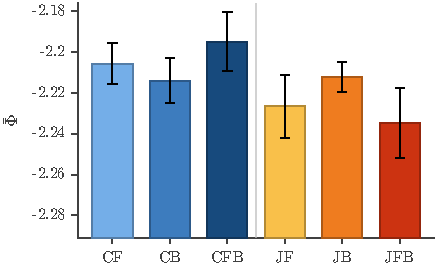
\includegraphics[width=\linewidth]{results/res_Phi.pdf}\caption{Movement smoothness}\label{fig:resPhi}\end{subfigure}\hfill
\begin{subfigure}[t]{0.485\linewidth}\centering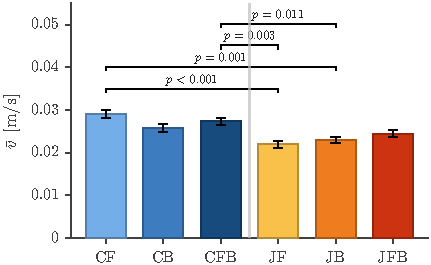
\includegraphics[width=\linewidth]{results/res_vbar.pdf}\caption{Mean hand speed}\label{fig:resv}\end{subfigure}
\vspace{0.35em}
\begin{subfigure}[t]{0.485\linewidth}\centering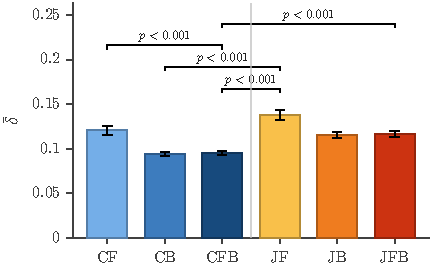
\includegraphics[width=\linewidth]{results/res_deltabar.pdf}\caption{Mean tracking slack}\label{fig:resdelta}\end{subfigure}\hfill
\begin{subfigure}[t]{0.485\linewidth}\centering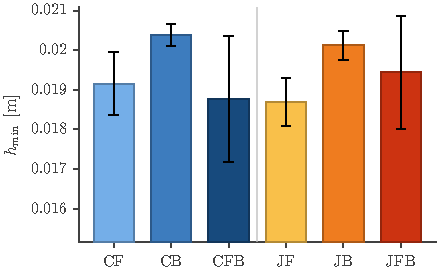
\includegraphics[width=\linewidth]{results/res_hmin.pdf}\caption{Minimum clearance}\label{fig:reshmin}\end{subfigure}
\vspace{0.35em}
\begin{subfigure}[t]{0.485\linewidth}\centering
\includegraphics{results/res_Tlambda.pdf}\caption{Filter active time}\label{fig:resTlam}\end{subfigure}\hfill
\begin{subfigure}[t]{0.485\linewidth}\centering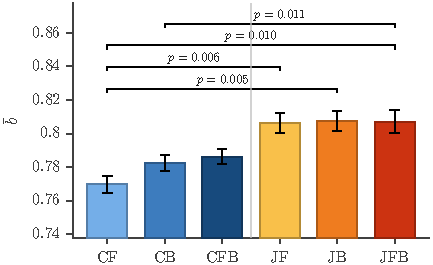
\includegraphics[width=\linewidth]{results/res_bbar.pdf}\caption{Mean intent confidence}\label{fig:resb}\end{subfigure}
\caption{Condition means with the standard error of the mean; brackets mark the Holm-corrected significant pairs. Symbols and units are defined in Sections~\ref{sec:resperf}--\ref{sec:resauthority}.}
\label{fig:resmain}
\end{figure}

\begin{figure}[p]
\centering
\begin{subfigure}[t]{0.485\linewidth}\centering
\includegraphics{results/res_rho.pdf}\caption{Operator--policy agreement}\label{fig:resrho}\end{subfigure}\hfill
\begin{subfigure}[t]{0.485\linewidth}\centering
\includegraphics{results/res_phialpha.pdf}\caption{Autonomy-led time}\label{fig:resphi}\end{subfigure}
\vspace{0.35em}
\begin{subfigure}[t]{0.485\linewidth}\centering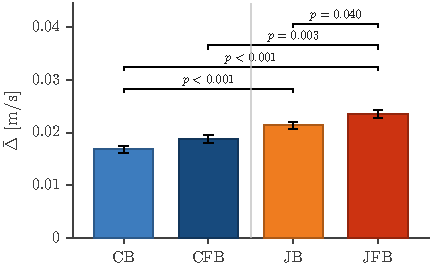
\includegraphics[width=\linewidth]{results/res_Dmean.pdf}\caption{Mean command alteration}\label{fig:resDmean}\end{subfigure}\hfill
\begin{subfigure}[t]{0.485\linewidth}\centering
\includegraphics[width=\linewidth]{results/res_Dpeak.pdf}\caption{Peak command alteration}\label{fig:resDpeak}\end{subfigure}
\vspace{0.35em}
\begin{subfigure}[t]{0.485\linewidth}\centering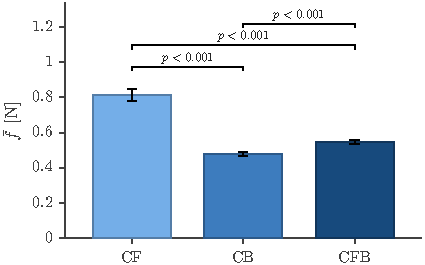
\includegraphics{results/res_fbarC.pdf}\caption{Rendered force, clutch}\label{fig:resfC}\end{subfigure}\hfill
\begin{subfigure}[t]{0.485\linewidth}\centering
\includegraphics[width=\linewidth]{results/res_fbarJ.pdf}\caption{Rendered force, joystick}\label{fig:resfJ}\end{subfigure}
\vspace{0.35em}
\begin{subfigure}[t]{0.485\linewidth}\centering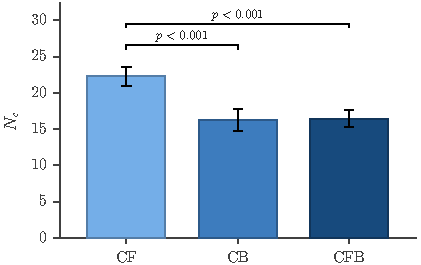
\includegraphics{results/res_Nc.pdf}\caption{Re-indexing operations}\label{fig:resNc}\end{subfigure}\hfill
\begin{subfigure}[t]{0.485\linewidth}\centering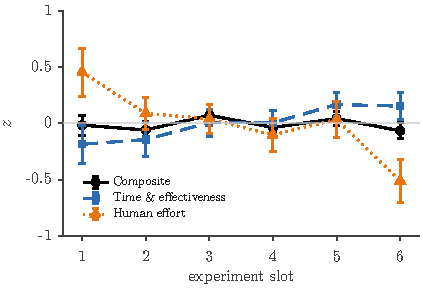
\includegraphics{results/res_learn_slot.pdf}\caption{Score along the session}\label{fig:reslearnslot}\end{subfigure}
\caption{Panels (a) to (d) exist only where blending is active and show four conditions; (e) to (g) compare assistance inside one mapping and their levels are not comparable across panels; (h) tracks three standardised scores over the session.}
\label{fig:resextra}
\end{figure}

\subsection{Learning effect}
\label{sec:reslearning}

The counterbalanced order of Section~\ref{sec:studyprocedure} balances the mode averages but not practice, so two checks test whether learning contaminates the comparisons above, the first reported in panel (h) of Figure~\ref{fig:resextra}.

The first asks whether performance drifts along the session. The composite score, obtained by averaging the standardised family scores, is flat: its slope over the six slots is not significant, so the study as a whole shows no overall practice trend. Two families do drift, in opposite directions. Time and effectiveness improves, which is the expected shape of learning, while operator effort deteriorates, that is, participants work the handle harder by the end of the session than at its beginning. Fatigue is the natural reading of a measure that worsens monotonically while task performance improves, and it is a caution for any effort claim that relies on ordering.

The second check asks whether the difference between the two modes depends on which of them a participant meets first. Splitting the twenty-four participants into the twelve who meet the clutch mapping first and the twelve who meet the joystick mapping first, the joystick-minus-clutch difference in composite score is statistically indistinguishable between the two groups, $p = 0.544$ by rank-sum test, the two group means differing by less than a tenth of a standard deviation. This is the single most important number for the mode conclusion, because it establishes that the advantage is not an artefact of practice accumulated before the second mode is reached. The same check fails, however, for the time-and-effectiveness and operator-effort families, which is why no claim in Section~\ref{sec:resperf} rests on task time alone, and why the speed comparison between modes is reported there as undetermined rather than as a result.






\begin{table}[p]
\centering
\footnotesize
\caption[Assumption checks and analysis-of-variance outcomes for every reported measure]{Assumption checks and analysis-of-variance outcomes for every reported measure, one line per tested effect. Symbols are defined with the corresponding measure in Sections~\ref{sec:resperf}--\ref{sec:reseffort}; the value in parentheses after each symbol is the $p$ value of the Shapiro--Wilk test on the residuals of the two-way model, one test per measure. Mauchly's $p$ and the Greenhouse--Geisser $\varepsilon$ are those of the effect on the line, the interaction carrying its own; where Mauchly rejects sphericity at $0.05$ the degrees of freedom of $F$ are the adjusted ones, $\varepsilon\,\mathrm{df}$, and the $p$ value is the corrected one. A dash marks a factor with two levels, for which sphericity holds by construction. The last column is the $p$ value of the aligned-rank-transform analysis of the same effect~\cite{wobbrock2011art}, or the Friedman $p$ value for the one-way measures $\bar f$ and $N_c$, which are compared within one mapping only.}
\label{tab:assumptions}
\setlength{\tabcolsep}{3.5pt}\scriptsize
\begin{tabular}{@{}llcccccc@{}}
\toprule
Measure (SW $p$) & Effect & Mauchly $p$ & $\varepsilon$ & $F(\mathrm{df}_1,\mathrm{df}_2)$ & $p$ & $\eta^2_p$ & ART / Friedman $p$ \\
\midrule
$T$ ($0.415$) & Mode & --- & --- & $F(1,23)=0.93$ & $0.345$ & $0.04$ & $0.169$ \\
 & Assist. & $0.180$ & $0.87$ & $F(2,46)=64.53$ & $<0.001$ & $0.74$ & $<0.001$ \\
 & Mode$\times$Assist. & $0.007$ & $0.73$ & $F(1.47,33.80)=4.23$ & $0.033$ & $0.16$ & $0.007$ \\
\addlinespace[2pt]
$L$ ($<0.001$) & Mode & --- & --- & $F(1,23)=12.31$ & $0.002$ & $0.35$ & $<0.001$ \\
 & Assist. & $<0.001$ & $0.67$ & $F(1.34,30.73)=75.84$ & $<0.001$ & $0.77$ & $<0.001$ \\
 & Mode$\times$Assist. & $0.008$ & $0.74$ & $F(1.48,34.00)=2.78$ & $0.090$ & $0.11$ & $0.099$ \\
\addlinespace[2pt]
$\bar{\Phi}$ ($0.004$) & Mode & --- & --- & $F(1,23)=2.66$ & $0.116$ & $0.10$ & $0.276$ \\
 & Assist. & $0.165$ & $0.87$ & $F(2,46)=0.03$ & $0.969$ & $0.00$ & $0.870$ \\
 & Mode$\times$Assist. & $0.029$ & $0.78$ & $F(1.57,36.06)=1.40$ & $0.257$ & $0.06$ & $0.294$ \\
\addlinespace[2pt]
$\bar{v}$ ($0.217$) & Mode & --- & --- & $F(1,23)=25.24$ & $<0.001$ & $0.52$ & $<0.001$ \\
 & Assist. & $0.389$ & $0.92$ & $F(2,46)=2.83$ & $0.070$ & $0.11$ & $0.129$ \\
 & Mode$\times$Assist. & $0.182$ & $0.87$ & $F(2,46)=14.23$ & $<0.001$ & $0.38$ & $<0.001$ \\
\addlinespace[2pt]
$\bar{\delta}$ ($<0.001$) & Mode & --- & --- & $F(1,23)=37.21$ & $<0.001$ & $0.62$ & $<0.001$ \\
 & Assist. & $0.005$ & $0.73$ & $F(1.45,33.40)=40.01$ & $<0.001$ & $0.64$ & $<0.001$ \\
 & Mode$\times$Assist. & $0.010$ & $0.75$ & $F(1.49,34.34)=0.26$ & $0.707$ & $0.01$ & $0.555$ \\
\addlinespace[2pt]
$h_{\min}$ ($<0.001$) & Mode & --- & --- & $F(1,23)=0.00$ & $0.983$ & $0.00$ & $0.640$ \\
 & Assist. & $<0.001$ & $0.68$ & $F(1.35,31.13)=1.36$ & $0.262$ & $0.06$ & $0.091$ \\
 & Mode$\times$Assist. & $<0.001$ & $0.60$ & $F(1.20,27.69)=0.18$ & $0.722$ & $0.01$ & $0.440$ \\
\addlinespace[2pt]
$T_{\lambda}$ ($<0.001$) & Mode & --- & --- & $F(1,23)=17.20$ & $<0.001$ & $0.43$ & $<0.001$ \\
 & Assist. & $0.069$ & $0.82$ & $F(2,46)=25.32$ & $<0.001$ & $0.52$ & $<0.001$ \\
 & Mode$\times$Assist. & $0.015$ & $0.76$ & $F(1.52,34.93)=0.82$ & $0.420$ & $0.03$ & $0.398$ \\
\addlinespace[2pt]
$\bar{b}$ ($0.131$) & Mode & --- & --- & $F(1,23)=34.83$ & $<0.001$ & $0.60$ & $<0.001$ \\
 & Assist. & $0.152$ & $0.86$ & $F(2,46)=1.73$ & $0.189$ & $0.07$ & $0.237$ \\
 & Mode$\times$Assist. & $0.550$ & $0.95$ & $F(2,46)=1.83$ & $0.172$ & $0.07$ & $0.216$ \\
\addlinespace[2pt]
$\rho$ ($0.011$) & Mode & --- & --- & $F(1,23)=167.6$ & $<0.001$ & $0.88$ & $<0.001$ \\
 & Assist. & --- & --- & $F(1,23)=20.29$ & $<0.001$ & $0.47$ & $<0.001$ \\
 & Mode$\times$Assist. & --- & --- & $F(1,23)=10.09$ & $0.004$ & $0.30$ & $<0.001$ \\
\addlinespace[2pt]
$\phi_\alpha$ ($0.851$) & Mode & --- & --- & $F(1,23)=256.2$ & $<0.001$ & $0.92$ & $<0.001$ \\
 & Assist. & --- & --- & $F(1,23)=20.21$ & $<0.001$ & $0.47$ & $<0.001$ \\
 & Mode$\times$Assist. & --- & --- & $F(1,23)=18.70$ & $<0.001$ & $0.45$ & $<0.001$ \\
\addlinespace[2pt]
$\bar{\Delta}$ ($0.432$) & Mode & --- & --- & $F(1,23)=29.93$ & $<0.001$ & $0.57$ & $<0.001$ \\
 & Assist. & --- & --- & $F(1,23)=10.40$ & $0.004$ & $0.31$ & $0.003$ \\
 & Mode$\times$Assist. & --- & --- & $F(1,23)=0.04$ & $0.835$ & $0.00$ & $0.489$ \\
\addlinespace[2pt]
$\Delta_{\max}$ ($<0.001$) & Mode & --- & --- & $F(1,23)=36.37$ & $<0.001$ & $0.61$ & $<0.001$ \\
 & Assist. & --- & --- & $F(1,23)=4.62$ & $0.042$ & $0.17$ & $0.014$ \\
 & Mode$\times$Assist. & --- & --- & $F(1,23)=2.84$ & $0.105$ & $0.11$ & $0.031$ \\
\addlinespace[2pt]
$\bar{f}$ (clutch) ($0.477$) & Assist. & $<0.001$ & $0.66$ & $F(1.31,30.14)=75.70$ & $<0.001$ & $0.77$ & $<0.001$ \\
\addlinespace[2pt]
$\bar{f}$ (joystick) ($0.439$) & Assist. & $0.160$ & $0.87$ & $F(2,46)=1.71$ & $0.193$ & $0.07$ & $0.311$ \\
\addlinespace[2pt]
$N_c$ ($0.917$) & Assist. & $0.592$ & $0.96$ & $F(2,46)=17.82$ & $<0.001$ & $0.44$ & $<0.001$ \\
\bottomrule
\end{tabular}
\end{table}

\FloatBarrier
\subsection{Subjective experience}
\label{sec:ressubj}

Twenty-four volunteers take part, eighteen men and five women, one of whom does not return the opening form. Ages range from $20$ to $58$~years, with a mean of $28.0$ and a standard deviation of $7.7$ over the twenty-two who report one. Twenty are right-handed and three report no strong hand preference. Self-rated familiarity with teleoperation devices averages $2.3$ on a five-point scale, with eleven participants placing themselves at the lowest level and six in the top two, so the sample is predominantly inexperienced. Every participant returns all six condition forms and the closing form, which yields 144 condition reports with no missing rating and forty-eight complete preference rankings.

The questionnaire is administered once per condition, after the participant has attempted that condition on both scenarios, and carries six items answered on a seven-point ordinal scale: three workload items drawn from the NASA task load index~\cite{hart1988nasatlx} and three human--robot-interaction items, of which the trust item follows Jian, Bisantz, and Drury~\cite{jian2000trust}. Mental demand $S_{\mathrm{md}}$ and physical demand $S_{\mathrm{pd}}$ are costs, on which a high score is unfavourable. Perceived success $S_{\mathrm{pf}}$, the sense of being in control of the robot's motion $S_{\mathrm{ct}}$, trust that the robot does what is intended $S_{\mathrm{tr}}$, and the judgement that the motion is smooth and comfortable $S_{\mathrm{sm}}$ are benefits, on which a high score is favourable. Reversing the two demand items as $8-S$ and averaging all six yields one subjective quality index $\bar{S}$ per condition, on the same seven-point scale and oriented so that a higher value denotes a better experience; the items are consistent enough for that summary to carry meaning, with Cronbach's $\alpha = 0.853$ over the 144 reports. Because the responses are ordinal, they are examined with the rank procedure of Section~\ref{sec:stats} alone, and Kendall's coefficient of concordance $W_{\mathrm{K}}$ accompanies each Friedman test as the magnitude of its effect.

\begin{figure}[t]
\centering
\begin{subfigure}[t]{0.32\linewidth}\centering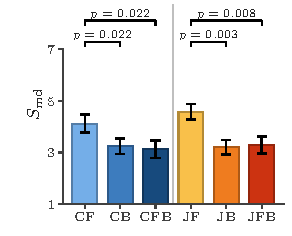
\includegraphics[width=\linewidth]{results/res_subj_md.pdf}\caption{Mental demand}\label{fig:subjmd}\end{subfigure}\hfill
\begin{subfigure}[t]{0.32\linewidth}\centering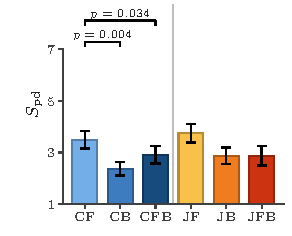
\includegraphics[width=\linewidth]{results/res_subj_pd.pdf}\caption{Physical demand}\label{fig:subjpd}\end{subfigure}\hfill
\begin{subfigure}[t]{0.32\linewidth}\centering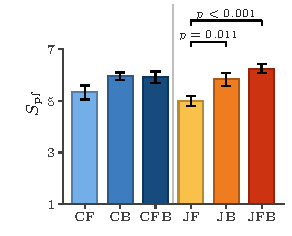
\includegraphics[width=\linewidth]{results/res_subj_pf.pdf}\caption{Perceived success}\label{fig:subjpf}\end{subfigure}
\vspace{0.35em}
\begin{subfigure}[t]{0.32\linewidth}\centering
\includegraphics[width=\linewidth]{results/res_subj_ct.pdf}\caption{Sense of control}\label{fig:subjct}\end{subfigure}\hfill
\begin{subfigure}[t]{0.32\linewidth}\centering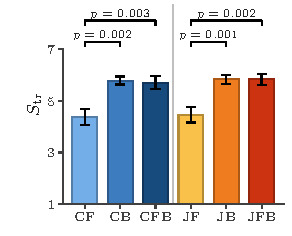
\includegraphics[width=\linewidth]{results/res_subj_tr.pdf}\caption{Trust}\label{fig:subjtr}\end{subfigure}\hfill
\begin{subfigure}[t]{0.32\linewidth}\centering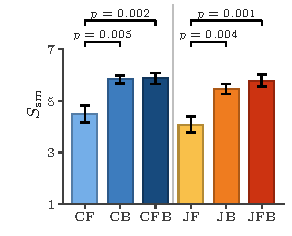
\includegraphics[width=\linewidth]{results/res_subj_sm.pdf}\caption{Motion comfort}\label{fig:subjsm}\end{subfigure}
\caption{Questionnaire responses by condition, as means over the twenty-four participants with the standard error of the mean. Every item is answered on the same scale, running from $1$ at the axis floor to $7$; the vertical rule separates the clutch mapping from the joystick mapping, and the conditions are coded as in Table~\ref{tab:cells}. Brackets above the scale give the Holm-corrected Wilcoxon $p$ values of the two contrasts against force guidance alone within each mapping. Symbols are defined in the text.}
\label{fig:ressubj}
\end{figure}

\begin{table}[t]
\centering
\small
\caption{Effect of the assistance channel on each questionnaire item, collapsed over the two mappings, under force guidance alone (F), reference blending alone (B), and both together (FB). The Friedman test runs over those three settings, with Kendall's coefficient of concordance $W_{\mathrm{K}}$ as its effect size, and the last three columns are Holm-corrected Wilcoxon $p$ values. $\bar{S}$ is the composite index; a high score is unfavourable for $S_{\mathrm{md}}$ and $S_{\mathrm{pd}}$ and favourable otherwise. Symbols are defined in Section~\ref{sec:ressubj}.}
\label{tab:subjassist}
\begin{tabular}{lcccccccccc}
\toprule
 & \multicolumn{3}{c}{Mean rating} & \multicolumn{3}{c}{Friedman} & \multicolumn{3}{c}{Holm-corrected $p$} \\
\cmidrule(lr){2-4}\cmidrule(lr){5-7}\cmidrule(lr){8-10}
 & F & B & FB & $\chi^2(2)$ & $p$ & $W_{\mathrm{K}}$ & F--B & F--FB & B--FB \\
\midrule
$S_{\mathrm{md}}$ & $4.35$ & $3.23$ & $3.21$ & $19.50$ & $<0.001$ & $0.41$ & $0.002$   & $0.002$   & $0.985$ \\
$S_{\mathrm{pd}}$ & $3.62$ & $2.62$ & $2.90$ & $18.30$ & $<0.001$ & $0.38$ & $0.008$   & $0.009$   & $0.062$ \\
$S_{\mathrm{pf}}$ & $5.17$ & $5.90$ & $6.08$ & $17.26$ & $<0.001$ & $0.36$ & $0.003$   & $0.004$   & $0.154$ \\
$S_{\mathrm{ct}}$ & $4.54$ & $5.77$ & $5.65$ & $17.46$ & $<0.001$ & $0.36$ & $<0.001$  & $0.008$   & $0.818$ \\
$S_{\mathrm{tr}}$ & $4.42$ & $5.81$ & $5.77$ & $24.21$ & $<0.001$ & $0.50$ & $<0.001$  & $<0.001$  & $0.873$ \\
$S_{\mathrm{sm}}$ & $4.29$ & $5.65$ & $5.83$ & $22.07$ & $<0.001$ & $0.46$ & $0.001$   & $<0.001$  & $0.180$ \\
\midrule
$\bar{S}$         & $4.41$ & $5.55$ & $5.54$ & $27.85$ & $<0.001$ & $0.58$ & $<0.001$  & $<0.001$  & $0.987$ \\
\bottomrule
\end{tabular}
\end{table}

\begin{figure}[t]
\centering
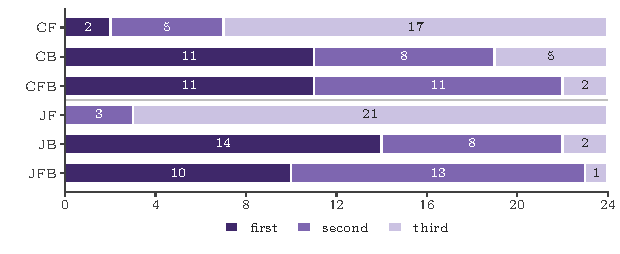
\includegraphics{results/res_subj_ranks.pdf}
\caption{Preference ranking of the three assistance settings within each mapping, as the number of the twenty-four participants placing each condition first, second, or third. The horizontal axis counts participants, so every row sums to twenty-four, and every segment is annotated with its own count. The horizontal rule separates the clutch mapping from the joystick mapping, and the conditions are coded as in Table~\ref{tab:cells}.}
\label{fig:subjranks}
\end{figure}

Figure~\ref{fig:ressubj} reports every item in every condition, and one pattern governs all six. The assistance channel separates the conditions, it separates them in the same direction under both mappings, and force guidance alone is the least favourable of the three settings on every item. Table~\ref{tab:subjassist} gives the statistics collapsed over the mapping. The Friedman test rejects for all six items and for the index, with $W_{\mathrm{K}}$ between $0.36$ and $0.58$, a large effect for a within-subject design of this size, and the index rises from $4.41$ under force guidance alone to $5.55$ under blending and $5.54$ under both channels together.

Two features of that pattern matter more than the omnibus result. The first is which items move most. Blending removes authority from the operator, yet the two items it raises most are precisely the ones that a loss of authority might have been expected to cost: the sense of control climbs from $4.54$ to $5.77$, and trust from $4.42$ to $5.81$. Participants do not experience the arbitration as authority taken away but as the robot doing what they mean. The second is what does not move. Blending alone and blending with force guidance are indistinguishable on every item and on the index, the corrected $p$ never falling below $0.06$, so no evidence is found that the haptic channel adds anything the operator can detect once the reference is already being blended. The one exception is physical demand inside the clutch mapping, where the two blended settings do differ, $p = 0.026$; it has no counterpart under the joystick mapping and does not survive collapsing the two.

No subjective difference between the two mappings is detected. None of the six items separates the two, and neither does the index, which differs by $0.13$ points in favour of the clutch mapping, $p = 0.498$. The largest of the seven contrasts is motion comfort, at $0.29$ points, and it too favours the clutch mapping, $p = 0.092$. This deserves to be stated against the objective record, because the two disagree: the joystick mapping produces the shorter hand path $L$ and the more confident intent estimate $\bar{b}$, yet none of that advantage appears in what the operators report, and the one subjective trend that does appear points the other way.



Ranking the three assistance settings inside each mapping reproduces that result through a different question format. Figure~\ref{fig:subjranks} gives the distributions. Force guidance alone is placed last by seventeen of the twenty-four participants under the clutch mapping and by twenty-one of twenty-four under the joystick mapping, where it draws no first place at all. The two blended settings are again indistinguishable from one another, $p = 0.663$ in both mappings, so the ordering the ratings establish is confirmed by an instrument that forces a choice rather than inviting a score.

Asked at the end of the session which of the two mappings is the better overall, thirteen participants choose the clutch and eleven the joystick, an even split, exact binomial $p = 0.839$. The question offers no neutral option, so the count cannot separate a divided population from an indifferent one; read together with the flat index contrast above, indifference is at least as plausible a reading as division.

%───────────────────────────────────────────────────────────────────────────────

\chapter{Discussion}
\label{ch:discussion}

Chapter~\ref{ch:exp} reported what the hardware trials and the human-subject study measured; this chapter reads those results against the hypotheses of Section~\ref{sec:rqs}, weighs the alternative explanations the design does not rule out, and states the threats to validity that qualify every claim above.

\section{Findings against expectations}
\label{sec:discussion-expectations}

\textbf{H1} is rejected in the shape it predicted, although the interaction it predicted is real on one of its two named measures. The mode--assistance interaction on task time is significant (Table~\ref{tab:assumptions}), so the two mappings do respond differently to the assistance channel, but not as the reversal H1 stated: force guidance alone is the slowest setting under \emph{both} mappings, not only under joystick, so CF never leads the clutch mapping (Section~\ref{sec:resperf}); the corresponding interaction on path length, where the same clutch-side reasoning applies, is not significant ($p=0.090$). The clutch-side mechanism did not survive contact with the operators either: the pull toward the goal was reported as a force to resist, not a depth cue, and within the clutch mapping it is blending, not guidance, that lowers both the rendered force and the number of re-indexing operations (Section~\ref{sec:reseffort}). The joystick-side half fares better in ranking --- JF is the single slowest of the six conditions and JFB the single quickest --- and its channel-congruence mechanism is corroborated by a measure H1 did not name: operator--policy agreement $\rho$ shows an interaction of its own, the gain from adding guidance to blending several times larger under joystick than under clutch (Section~\ref{sec:resauthority}). That finding supports the reasoning behind H1's joystick half without confirming the time prediction itself, and the two channels together produce no detectable objective or subjective gain of FB over B in either mapping.

\textbf{H2} is not supported on either of its named measures. No mode effect on task time survives the practice check of Section~\ref{sec:reslearning}; where the objective record separates the mappings at all it leans the other way, the joystick mapping yielding the shorter hand path and the more confident intent estimate, while the clutch mapping's faster hand speed is spent on longer paths cut into about three times as many separate driving segments (Section~\ref{sec:resperf}); and the subjective composite index $\bar{S}$ shows no mode difference either, $p=0.498$, with the closing preference split at thirteen to eleven (Section~\ref{sec:ressubj}). The one-to-one correspondence between hand and gripper was as intuitive as expected once in motion, but the re-indexing procedure around it was not: several participants found the clutch sequence confusing and occasionally pressed the wrong button, an observation made during the sessions rather than a recorded measure, and the time and effort this procedure costs is what the objective measures register in place of the predicted advantage.

\textbf{H3} is rejected on both named measures, and in the opposite direction to the one predicted. Both workload subscales fall, rather than rise, under blending: mental demand from $4.35$ under force guidance alone to $3.21$--$3.23$ under the two blended settings, and physical demand from $3.62$ to $2.62$--$2.90$, every contrast Holm-corrected significant (Table~\ref{tab:subjassist}). The same two blended settings also raise the authority-cost items a felt intervention was expected to threaten: the sense of control climbs from $4.54$ to $5.77$ and trust from $4.42$ to $5.81$, and both are ranked ahead of guidance alone by nearly every participant (Figure~\ref{fig:subjranks}). The disturbance the hypothesis anticipated was felt, but on the other channel: operators described the guidance force, not the blended reference, as working against them and as overriding their intention, and some resisted it outright, while the blending correction --- although less counterable in principle, since the only way to oppose it is to move away from the goal --- drew few complaints. The scenario-specific half of H3 remains untested by design: the two scenarios are averaged into one value per condition before any statistic is computed (Section~\ref{sec:discussion-threats}), so no claim here is made about whether the effect is sharper in the cluttered relay scenario than in the independent one.

\textbf{H4} is supported on every named measure and exceeds its own stated scope. Blending lowers path length by about a third, tracking slack by about a quarter, and filter active time by about a third relative to guidance alone, while the attained clearance does not move (Sections~\ref{sec:resperf} and~\ref{sec:ressafety}). Task time, on which the hypothesis predicted no direction, falls with the others by about a quarter, so the correction of the executed trajectory paid in speed as well as in the quality H4 named.

Two findings fall outside all four hypotheses. The two transparency measures, mean and peak command alteration (Section~\ref{sec:resauthority}), disagree in direction between the mappings, and this is read here as a genuine finding about how arbitration behaves differently under a continuous-velocity mapping and a re-indexed position mapping, not as a contradiction to be explained away. The null result on minimum clearance (Section~\ref{sec:ressafety}) is read as the barrier itself setting an unmoving floor, consistent with its design, and not as evidence that the six conditions are equally safe in every other respect.

\section{Alternative explanations}
\label{sec:discussion-alternatives}

Several results admit an explanation other than the one Section~\ref{sec:conclfindings} states as the leading reading. The deficit of force guidance alone could reflect how its saturation was calibrated (Section~\ref{sec:study}) --- absolute in the clutch mapping, deadzone-exit-calibrated in the joystick mapping --- rather than a property of haptic guidance as a channel; a different calibration could narrow or widen the gap to blending. Blending's advantage on the subjective measures could be partly attributable to the visible reference marker, the colour cue that turns from orange to green as authority shifts (Section~\ref{sec:studyenv}), rather than to the arbitration law itself: the cue is present only in the blended conditions, so it is confounded with the channel under test. The joystick mapping's higher intent-estimator confidence (Section~\ref{sec:resauthority}) is a property of the estimator's own evidence stream --- a continuous velocity command supplies it steadily, a re-indexed position command interrupts it --- and need not reflect the operator's own intent being any clearer under one mapping than the other. The belief score's own competition-normalisation (Section~\ref{sec:belief}) can inflate apparent confidence once one goal candidate is even slightly ahead of its rivals, so the confidence measure may overstate how resolved the operator's intent actually was. The absence of a subjective mapping effect could be a ceiling or an order effect rather than genuine indifference, since ratings cluster toward the favourable end of the scale and mapping order was blocked rather than fully randomised (Section~\ref{sec:reslearning}). Finally, the monotonic worsening of operator effort across the session (Section~\ref{sec:reslearning}) is read here as fatigue, but a rising familiarity with how hard the handle can safely be pushed is not excluded by the data.

\section{Threats to validity}
\label{sec:discussion-threats}

\textbf{Internal.} Mapping order was blocked --- the three conditions of one mapping run before the three of the other, order balanced across participants --- rather than interleaved; the order check found the mode difference in composite score independent of which mapping came first ($p = 0.544$), but the same check failed for task time and for operator effort (Section~\ref{sec:reslearning}), so those two families carry a residual order risk the composite score does not. The two scenarios are averaged into one value per participant per condition, which cannot separate an effect specific to one scenario from a genuine main effect. No unassisted baseline was run, so no result here claims that assistance beats no assistance, only that the assistance channels differ from one another. The three-level assistance design (F, B, FB) does not realise the full $2\times2$ of the two channels, so channel main effects and their interaction are not separately estimable, only the F-versus-FB and B-versus-FB contrasts.

\textbf{Construct.} The rendered-force and re-indexing measures are not comparable across mappings, because the clutch tether and the joystick centring spring encode different physical quantities through the same actuator (Section~\ref{sec:reseffort}). The minimum clearance floor is a property of the barrier's own design margin, not of operator skill, which limits what that measure can be read to say about the assistance. Throughout, a non-significant test is treated as absence of evidence rather than evidence of equivalence, given $n=24$. The mode$\times$assistance interaction on peak command alteration flips significance between the corrected analysis of variance and the aligned rank transform (Section~\ref{sec:stats}); no claim in this thesis rests on that interaction.

\textbf{External.} The sample is twenty-four novices, predominantly male and reporting low prior familiarity with teleoperation devices (Section~\ref{sec:ressubj}), so the subjective preferences do not generalise to an experienced operator population without further evidence. The factorial comparison itself ran only in a matched simulation environment. The two hardware trials used a different, full-size haptic device and the robot's own live, camera-perceived world rather than the study's declared one (Section~\ref{sec:hwteleop}), so they corroborate the architecture's mechanisms without replicating the factorial result at hardware scale. The operator's picture throughout the study was a five-window display (Section~\ref{sec:studyapparatus}), a specific instrumentation choice that a different display configuration might not reproduce.

\textbf{Missing ablations.} Neither the alignment-based arbitration nor the adaptive dual-variable scheduling was isolated by ablation: no run compares the alignment law against a confidence- or distance-based arbitration rule, and no run compares the adaptive slack schedule against a fixed-weight baseline. Both mechanisms are implemented and exercised throughout Chapter~\ref{ch:exp}, but neither is shown here to outperform the alternative it was chosen over.

%───────────────────────────────────────────────────────────────────────────────

\chapter{Conclusions}
\label{ch:conclusions}

This thesis set out to reconcile two demands that are often treated as in tension: that a teleoperated bimanual manipulator be assisted enough to be usable through a single grounded haptic interface, and that the assistance never be trusted to keep the operator safe on its own. The two demands are kept apart architecturally rather than balanced numerically --- a reactive safety filter enforces collision avoidance and joint limits as hard constraints on whatever command reaches the arms, and an alignment-based arbitration law decides, moment to moment, how much of the operator's own hand the assistance is allowed to move --- and this chapter takes stock of what evaluating that architecture, on the physical robot and at human-subject-study scale, actually shows, building on the reading of those results against expectations, the alternative explanations, and the threats to validity that Chapter~\ref{ch:discussion} already sets out.

Four design commitments carry that architecture through to evaluation. The safety filter is a single strictly convex QP, formulated natively in joint velocity rather than in the position-space updates the closest prior systems use, with a normalised CLF that lets tracking degrade gracefully under conflict while the CBF rows never do (Section~\ref{sec:clf}) --- the property the home-to-crossed hardware test of Section~\ref{sec:hwswap} is built specifically to exercise, and which it confirms directly: driven toward a target pair that is not jointly reachable, the two arms do not stall or fight the barrier, they converge on the best pose their own scheduled slack weight admits. Authority over that filter's input is arbitrated on the instantaneous alignment between the operator's twist and a belief-weighted policy, rather than on a scalar confidence or distance, so that a direct disagreement always hands full authority back to the operator; the human-subject study shows this is not merely a safe default but the mechanism participants actually prefer. The QP's own KKT shadow prices, besides certifying the barrier, are reused to schedule the per-arm tracking slack, while a separate reference limiter sitting upstream of the CLF bounds how large a decrease that row can be asked to make in a single tick, keeping the resulting tracking slack and transient inside a known range --- both mechanisms visible operating on hardware in Section~\ref{sec:hwswap}'s limiter traces and in the teleoperated trial of Section~\ref{sec:hwteleop} alike. And a grasped object passes through an explicit hybrid lifecycle --- excluded during the blind approach, relaxed-contact during closure, carried payload, and ramped reactivation on release --- each regime with its own admissible set and reset map, a lifecycle the teleoperated trial exercises through three real grasp windows, one of them a full success.

\section{Summary of findings}
\label{sec:conclfindings}

The factorial comparison isolates what actually drives objective performance: assistance, not the motion mapping, explains most of the variance in task time and path length, and within assistance the effect is carried by reference blending rather than by force guidance, which is consistently the weakest of the three settings in both mappings (Section~\ref{sec:resperf}). No significant difference separates the two blended conditions from one another, and where they interact mechanistically at all it is because a velocity mapping reads guidance force and blended twist through the same channel, an effect the position mapping does not share (Section~\ref{sec:resauthority}). Safety is the one measure on which no factor produces a detectable difference: the worst clearance recorded sits within the same few millimetres in all six conditions, consistent with the barrier setting the floor, even as the time spent actively holding that floor falls by a third under the best-assisted condition (Section~\ref{sec:ressafety}).

The subjective record complicates a purely objective reading. Participants rate the two blended conditions as more controllable and more trustworthy than force guidance alone, and rank them ahead of it almost unanimously, even though blending is precisely the channel that takes some authority away from the hand (Section~\ref{sec:ressubj}); the operators experience the arbitration as the robot doing what they mean, not as authority lost. The motion mapping shows the opposite pattern: despite separating the two objectively on smoothness, hand speed, and intent confidence, no rated item nor the composite index distinguishes the two, which is absence of evidence for a subjective difference rather than evidence of its absence. A preference for one mapping over the other, where it exists at all, does not track the measurements that are supposed to explain it.

The two hardware trials of Section~\ref{sec:hwvalidation} corroborate the same mechanisms outside simulation. The open-loop reaching test confirms that the CLF's slack yields gracefully under a genuinely infeasible joint target, holding the barrier throughout; the teleoperated trial carries a real grasp to completion under the same architecture the human-subject study evaluates, with the shared-autonomy telemetry --- belief, authority, and the grasp state machine --- behaving exactly as the simulated study's own account of those mechanisms predicts. The same trial is also where the architecture exposes the one recorded safety violation, this thesis' clearest limitation.

\section{Limitations}
\label{sec:concllimitations}

The barrier condition the QP certifies each tick is nominal: it is evaluated on the most recently available reading of the state, not a certified physical forward invariance of the sampled, disturbed, actuator-lagged closed loop. No discrete-time or robust sampled-data argument is supplied to close that gap: measurement-robust CBFs~\cite{cosner2021mrcbf} address uncertainty in the measured state but not the sampling gap itself, and a dedicated sampled-data result~\cite{breeden2021sampled} tightens the margin by a term this thesis' controller does not carry. The empirical size of the gap is what Section~\ref{sec:hwswap} and Section~\ref{sec:hwteleop} measure directly: a $-2.6$~mm margin dip recorded open-loop, and, far more severely, the teleoperated event below.

The teleoperated trial of Section~\ref{sec:hwteleop} also records the architecture's clearest limitation. During the second grasp attempt, the grasp state machine removed the gripper--target pair from the barrier for the blind insertion, by design, to permit the grasp, held it removed through the stall and a clearance-blind, fixed-duration retreat, and restored it on a timer onto an unresolved overlap. The shadow price is zero throughout the stall because the row does not exist to report anything; once re-armed, every recorded solve is feasible and satisfies its own row, yet the closed loop still fails to deliver the escape that row demands (Section~\ref{sec:cbf-scope}). The gap is therefore twofold: a discrete layer that suspends a constraint and restores it without a clearance test, and the nominal-versus-physical gap of the barrier itself once re-armed inside a violation. The current revision's clearance-gated recovery (Section~\ref{sec:grasp}) addresses the first, not the second. Chapter~\ref{ch:sota} already flags the general form of this risk --- that a formal safety guarantee at the QP level does not rule out degraded closed-loop behaviour one level of abstraction up~\cite{reis2021undesirable} --- and this trial is the first evidence, on this architecture, that the risk is not only theoretical.

Two narrower limitations follow directly from the architecture's own stated design choices. Grasp confirmation is purely kinematic, so a wedged or joint-limited retreat of the kind above is inferred from a stall rather than sensed directly (Section~\ref{sec:grasp}); and the questionnaire sample, while adequately powered for the within-subject comparisons it supports, is predominantly male and reports low prior familiarity with teleoperation devices (Section~\ref{sec:ressubj}), so the subjective preferences reported here should not be read as generalising to an experienced operator population without further evidence. The haptic loop follows standard passivity heuristics, but no passivity or stability analysis covers the complete loop, moving targets, guidance bias with cross-process latency, saturation, and slew limiting included, and the device's own damping is not characterised; stability is supported only by the absence of reported oscillation.

The adaptive slack-weight schedule of Section~\ref{sec:sched} is likewise exercised rather than isolated, since no closed-loop stability analysis of the schedule--QP--robot loop and no ablation against a fixed slack weight or a single-filter schedule are carried out, so only the two-filter design as built is evaluated here. Its sensitivity parameter $\beta$ is calibrated to one specific constraint normalisation: scaling the collision row's Jacobian and right-hand side by a common factor leaves the QP's solution unchanged but scales its dual variable inversely, so the shadow price the schedule reads is tied to that normalisation, not an invariant quantity; normalising it by the row's own gradient norm, not implemented here, would remove that dependency.

\section{Future work}
\label{sec:conclfuture}

Three directions follow from these limitations rather than from open questions in the architecture itself. The retreat--barrier interaction is the most concrete: coupling the grasp state machine's recovery motion to the same barrier gradient the QP already computes, rather than suspending that pair's barrier and restoring it on an unconditional timer, would close exactly the gap the teleoperated trial exposes, and the shadow-price burst that preceded the interpenetration is itself a plausible detector for triggering that coupled recovery before a margin is actually crossed. Tactile or force sensing at the gripper would let grasp confirmation, and the wedged-retreat case in particular, be sensed rather than inferred from a kinematic stall, complementing the purely kinematic account this thesis gives in Section~\ref{sec:grasp}. And the factorial comparison itself is the natural next replication target on physical hardware, at whatever scale a multi-session, multi-participant protocol on the real platform allows, to test whether the assistance effects Section~\ref{sec:results} reports in simulation --- and that the two hardware trials here already show operating through the same mechanisms --- persist at the same magnitude once a physical operator, not a simulated one, is driving a physical arm.

None of this reopens the trade-off the Motivation opened with. The reactive layer still never decides which object is intended or when a detour is the only way out of a dead end, and the operator's authority over any motion they oppose is never in question in the human-subject data or in the one hardware episode where it mattered most. What Section~\ref{sec:results} and Section~\ref{sec:hwvalidation} together show is a narrower and more useful thing than validation in the abstract: precision and safety are the robot's to supply, intent and judgement stay the operator's, and across a matched simulated study and two trials on physical hardware, they stay that way.

\section*{Code availability}
The software described in this thesis is available in two repositories: the robot-side stack --- safety controller, shared autonomy, grasp lifecycle, and head perception --- at \url{https://github.com/Robertorocco/triago_control}, and the operator-side stack --- device driver, teleoperation modes, and force managers --- at \url{https://github.com/Robertorocco/haption_teleoperation}.




\appendix
\chapter{Configuration parameters}
\label{app:config}


All parameter values live in centralised configuration modules (one per subsystem) and are reported here, grouped by function, in the same order as the corresponding sections of Chapter~\ref{ch:method}. Symbols refer to the equations of that chapter.

\begingroup\footnotesize

\section{Control loop}
\begin{tabularx}{\linewidth}{@{}lllX@{}}
\toprule
Symbol & Name & Value & Meaning \\
\midrule
$f_{\text{ctrl}}$ & \texttt{CONTROL\_FREQ\_DEFAULT} & 150~Hz & loop rate \\
--- & \texttt{PUBLISH\_EVERY\_N} & 2 & telemetry decimation \\
--- & \texttt{WATCHDOG\_TIMEOUT} & 0.5~s & stale-reference freeze \\
\bottomrule
\end{tabularx}

The QP is solved by the Goldfarb--Idnani dual active-set method, an exact finite algorithm with no tolerance parameter, and the loop-rate telemetry above is a window mean over $N = $~\texttt{PUBLISH\_EVERY\_N} ticks, doubled to 4 on the physical robot.

\section{CLF and task tracking}
\begin{tabularx}{\linewidth}{@{}lllX@{}}
\toprule
Symbol & Name & Value & Meaning \\
\midrule
$\gamma$ & \texttt{GAMMA\_CLF\_DEFAULT} & 0.75 & CLF rate \eqref{eq:clf} \\
$\gamma_{\max}$ & \texttt{GAMMA\_MAX} & 1.2 & CLF rate, held arm \\
$W_{\text{task}}$ & \texttt{TASK\_WEIGHTS\_6D} & $\mathrm{diag}(10,10,10,0.5,0.5,0.5)$ & task weights \eqref{eq:clf} \\
$W_{\text{task}}^{\text{grasp}}$ & \texttt{TASK\_WEIGHTS\_6D\_GRASP} & $\mathrm{diag}(10,10,10,2,2,2)$ & task weights, precision \\
$w_{\delta}^{\text{base}}, w_{\delta}^{\max}$ & \texttt{BASE/MAX\_WEIGHT\_SLACK} & 150.75 / 250 & slack-weight range \eqref{eq:slacksched} \\
$\beta$ & \texttt{BETA} & 0.2 & schedule sensitivity \eqref{eq:slacksched} \\
$\tau_{\lambda}$ & \texttt{SLACK\_FILTER\_TAU} & 0.15~s & shadow-price LPF \\
$\tau_{w}$ & \texttt{WEIGHT\_SLACK\_FILTER\_TAU} & 0.2~s & slack-weight LPF \eqref{eq:slacksched} \\
\bottomrule
\end{tabularx}

\section{CBF and collision avoidance}
\begin{tabularx}{\linewidth}{@{}lllX@{}}
\toprule
Symbol & Name & Value & Meaning \\
\midrule
$\alpha_s$ & \texttt{ALPHA\_SOFTMIN} & 60 & SoftMin sharpness \eqref{eq:softmin} \\
$\gamma_{\text{cbf}}$ & \texttt{GAMMA\_CBF} & 0.70 & barrier gain \eqref{eq:cbf} \\
$d_0$ & \texttt{D\_SAFE\_BASE} & 0.015~m & base margin \eqref{eq:dsafe} \\
$k_v$ & \texttt{K\_V\_SAFE} & 0.1~m$\cdot$s/rad & closing-speed gain \eqref{eq:dsafe}, $\tau_v = k_v/\ell_{\max} \approx$ 14--29~ms \eqref{eq:tauv} \\
--- & \texttt{DISTANCE\_FILTER\_THRESHOLD} & 0.15~m & pair activation radius \\
$K$ & \texttt{K\_MAX\_PAIRS} & 60 & closest pairs kept \\
--- & \texttt{CAPSULE\_RADIUS} & 0.06~m & arm-capsule radius \\
\bottomrule
\end{tabularx}

\section{QP cost and joint limits}
\begin{tabularx}{\linewidth}{@{}lllX@{}}
\toprule
Symbol & Name & Value & Meaning \\
\midrule
$\lambda$ & \texttt{DAMP} & 12 & joint-velocity damping \eqref{eq:cost} \\
$w_c$ & \texttt{W\_CENTER} & 0.96 & posture weight \eqref{eq:cost} \\
$k_g$ & \texttt{K\_GRADIENT} & 0.07 & posture gradient gain \\
$v_{\max}^{\text{post}}$ & \texttt{V\_MAX\_POSTURE} & 1.0~rad/s & posture reference clamp \\
--- & \texttt{POSTURE\_GRASP\_SCALE} & 0.05 & posture scale, precision phases \\
--- & \texttt{POSTURE\_SCALE\_TAU} & 0.2~s & posture-scale ramp \\
$\rho$ & \texttt{RATE\_WEIGHT} & 50 & rate-damping weight, near convergence \\
--- & \texttt{RATE\_WEIGHT\_GRASP} & 20 & rate-damping weight, relaxed \\
--- & \texttt{STALL\_ERR\_POS\_THRESH} & 0.10~m & $\rho$ switching threshold \\
--- & \texttt{RATE\_DAMPING\_VS\_MEASURED} & true & measured anchor \\
$k_p$ & \texttt{P\_GAIN\_LIMITS} & 1.8 & joint-limit gain \eqref{eq:jlbrake} \\
$b_0$ & \texttt{JOINT\_LIMIT\_BUFFER\_BASE} & 0.15~rad & base buffer \eqref{eq:jlbrake} \\
$k_b$ & \texttt{JOINT\_LIMIT\_K\_V} & 0.1~s & buffer velocity horizon \\
\bottomrule
\end{tabularx}

\section{Reference limiter}
\begin{tabularx}{\linewidth}{@{}lllX@{}}
\toprule
Symbol & Name & Value & Meaning \\
\midrule
$V_{\max}^{\text{lin}}$ & \texttt{GOV\_V\_MAX\_LIN} & 0.20~m/s & reference linear speed cap \\
$V_{\max}^{\text{ang}}$ & \texttt{GOV\_V\_MAX\_ANG} & 0.3~rad/s & reference angular speed cap \\
$E_{\max}^{\text{pos}}$ & \texttt{GOV\_E\_MAX\_POS} & 0.30~m & position-error bound \\
$E_{\max}^{\text{ori}}$ & \texttt{GOV\_E\_MAX\_ORI} & 1.0~rad & orientation-error bound \\
$A_{\max}^{\text{lin}}$ & \texttt{GOV\_A\_MAX\_LIN} & 0.75~m/s$^2$ & linear acceleration cap \\
$A_{\max}^{\text{ang}}$ & \texttt{GOV\_A\_MAX\_ANG} & 3.0~rad/s$^2$ & angular acceleration cap \\
\bottomrule
\end{tabularx}

\section{Shared autonomy}
\begin{tabularx}{\linewidth}{@{}lllX@{}}
\toprule
Symbol & Name & Value & Meaning \\
\midrule
$W$ & --- & $\mathrm{diag}(10,10,10,2,2,2)$ & twist metric \eqref{eq:policyqp}, \eqref{eq:cost-belief} \\
$w_{\text{pos}}$ & --- & 0.1 & position-cost weight \eqref{eq:cost-belief} \\
$K_p$ & --- & 0.5 & policy gain \eqref{eq:vgeo} \\
$v_{\max},\omega_{\max}$ & --- & 0.1~m/s, 0.3~rad/s & robot-policy saturation \\
$v_{\max}^{u},\omega_{\max}^{u}$ & --- & 0.04~m/s, 0.10~rad/s & user-policy saturation \\
$\beta_0$ & --- & 0.04 & belief step \eqref{eq:effgains} \\
$\alpha_0$ & --- & 0.995 & belief forgetting \eqref{eq:effgains} \\
$v_{\text{lo}}, v_{\text{hi}}$ & \texttt{BELIEF\_V\_LOW/HIGH} & 0.005 / 0.030~m/s & engagement ramp \eqref{eq:engagement} \\
$g_{\min}$ & --- & 0.05 & engagement floor \\
--- & \texttt{BELIEF\_WARMUP\_S} & 2.5~s & post-reset warm-up \\
$g_{\text{warmup}}^{\min}$ & \texttt{BELIEF\_WARMUP\_FLOOR} & 0.25 & warm-up floor \\
$B_{\text{obj}}^{\text{ent}}, B_{\text{obj}}^{\text{stay}}$ & \texttt{BELIEF\_ENTER/STAY} & 0.90 / 0.75 & grasp-trigger hysteresis \eqref{eq:objbelief} \\
$\alpha_{\min},\alpha_{\max}$ & \texttt{ALIGN\_ALPHA\_MIN/MAX} & 0.2 / 0.8 & authority ramp \eqref{eq:alpha} \\
$v_{\text{still}},\omega_{\text{still}}$ & --- & 0.005~m/s, 0.05~rad/s & stillness gate; also bounds $\mathcal{T}_a$ \eqref{eq:Ta} and $\mathcal{C}_{\mathrm{act}}$ \eqref{eq:mrho} \\
--- & \texttt{ALIGN\_ALPHA\_LPF\_COEFF} & 0.1 & authority LPF \\
$\tau_{\text{dir}}$ & \texttt{GOAL\_DIRECTION\_FILTER\_TAU} & 4.0~s & goal free-direction filter \\
--- & \texttt{SIDE\_STANDOFF\_FROM\_CENTER} & 0.03~m & side-grasp standoff \\
--- & \texttt{ORIENT\_LOCK\_NEAR/FAR} & 0.12 / 0.30~m & finger-orientation hysteresis \\
\bottomrule
\end{tabularx}

\section{Grasp lifecycle}
\begin{tabularx}{\linewidth}{@{}lllX@{}}
\toprule
Symbol & Name & Value & Meaning \\
\midrule
--- & \texttt{POS/ANG\_ERR\_ENTER} & 0.040~m / 0.16~rad & \textsc{Pre-Grasp} entry gate \\
--- & \texttt{POS/ANG\_ERR\_STAY} & 0.072~m / 0.224~rad & \textsc{Pre-Grasp} stay gate \\
--- & \texttt{ALIGN\_POS/ANG\_TOL} & 0.0209~m / 0.103~rad & \textsc{Align} standoff tolerance \\
--- & \texttt{ALIGN\_CENTERING\_TOL} & 20.7~mm & \textsc{Align} centring tolerance \\
--- & \texttt{GRASP\_CBF\_MARGIN} & $-0.08$~m & grasp margin allowance \\
--- & \texttt{GRASP\_CONTACT\_DEPTH\_TOP/SIDE} & $-0.030$ / $-0.032$~m & closure contact depth \\
--- & \texttt{GRASP\_INSERTION\_TRAVEL\_TOP/SIDE} & 0.09 / 0.068~m & insertion travel \\
--- & \texttt{ALIGN/GRASP\_APPROACH\_TIMEOUT\_S} & 12 / 15~s & phase timeouts \\
--- & \texttt{RELEASE\_RETREAT\_DISTANCE/VELOCITY} & 0.14~m, 0.10~m/s & release retreat (current revision) \\
--- & \texttt{RELEASE\_RETREAT\_MAX\_S} & 3.5~s & release retreat cap \\
--- & \texttt{ABORT\_RETREAT\_DISTANCE/VELOCITY} & 0.10~m, 0.05~m/s & abort retreat (current revision) \\
--- & \texttt{ABORT\_RETREAT\_MAX\_S} & 6.0~s & abort retreat cap \\
--- & \texttt{ATTACH\_RAMP\_S} & 3.0~s & attach/detach pair-set ramp duration \\
--- & \texttt{ATTACH\_RAMP\_SHIFT\_MAX} & 0.30~m & initial distance shift of a freshly attached or detached object \\
--- & \texttt{RECOVER\_RAMP\_S} & 1.5~s & post-abort margin ramp duration \\
--- & \texttt{RECOVER\_CONFIRM\_S} & 0.5~s & clearance debounce before the ramp \\
--- & \texttt{RECOVER\_SAFETY\_BUFFER} & 0.02~m & live-contact clamp during recovery \\
\bottomrule
\end{tabularx}

\section{Head perception and world convergence}
\begin{tabularx}{\linewidth}{@{}lllX@{}}
\toprule
Symbol & Name & Value & Meaning \\
\midrule
--- & \texttt{WORLD\_CONF\_MIN} & 0.85 & confidence floor \\
$c_{\min}$ & \texttt{WORLD\_MIN\_ARC\_COVERAGE} & 0.55 & arc-coverage floor \\
$\varepsilon_{\text{pos}}$ & \texttt{WORLD\_CONVERGE\_POS\_AMP} & 1~mm & centre band \eqref{eq:amplock} \\
$\varepsilon_{\text{dim}}$ & \texttt{WORLD\_CONVERGE\_DIM\_AMP} & 1.5~mm & radius/height band \eqref{eq:amplock} \\
$T_w$ & \texttt{WORLD\_CONVERGE\_WINDOW\_S} & 1.0~s & amplitude-lock window \\
--- & \texttt{WORLD\_EXPECTED\_CYLINDERS} & 2 & expected objects \\
--- & \texttt{INTEGRATE\_VEL\_THRESH} & 0.04~rad/s & head-settled gate \\
--- & \texttt{ACTIVE\_VISION\_TIME\_BUDGET\_S} & 45~s & active-vision time budget \\
--- & \texttt{ACTIVE\_VISION\_PLATEAU\_EPS} & 0.01 & coverage plateau threshold \\
--- & \texttt{ACTIVE\_VISION\_REFINE\_OFFSET} & 0.06~m & refine fixation offset \\
--- & \texttt{CYL\_RADIUS\_INFLATION} & 0~m & optional radius inflation, unused in all reported experiments \\
\bottomrule
\end{tabularx}

\section{Head active-arm tracking}
\begin{tabularx}{\linewidth}{@{}lllX@{}}
\toprule
Symbol & Name & Value & Meaning \\
\midrule
$\lambda_v$ & \texttt{LAMBDA\_VISUAL} & 2.5 & visual-servo gain \eqref{eq:headvel} \\
$\qdot_{\max}$ & \texttt{MAX\_VELOCITY} & 0.20~rad/s & head joint velocity cap \eqref{eq:headvel} \\
$Z^{\star}$ & \texttt{TARGET\_DISTANCE} & 0.7~m & camera stand-off \eqref{eq:headtask} \\
$\gamma_{\text{head}}$ & \texttt{GAMMA\_CBF\_HEAD} & 0.35 & head barrier gain \eqref{eq:headcbf} \\
$d_{\text{extra}}$ & \texttt{D\_SAFE\_HEAD\_EXTRA} & 0.03~m & head extra clearance \eqref{eq:headcbf} \\
$\gamma_{\text{fov}}$ & \texttt{GAMMA\_FOV} & 5.0 & FOV barrier gain \eqref{eq:headfov} \\
$m_{\text{fov}}$ & \texttt{FOV\_MARGIN} & 50~px & FOV barrier margin \eqref{eq:headfov} \\
$W_s$ & \texttt{W\_SLACK\_PIXELS/DEPTH} & $1.0$, $10^{4}$ & IBVS slack weights \eqref{eq:headqp} \\
$W_s$ (PBVS) & \texttt{W\_SLACK\_PBVS} & $10^{4}$ & PBVS slack weight \eqref{eq:headqp} \\
$\lambda_{h,i}$ & \texttt{JOINT\_WEIGHTS} & 5.0 & joint regularisation \eqref{eq:headqp} \\
$k_g^{\text{head}}$ & \texttt{K\_POSTURE\_GRADIENT} & 0.05 & head posture gain \\
--- & \texttt{V\_MAX\_POSTURE} & 0.15~rad/s & head posture clamp \\
--- & \texttt{K\_HOME} & 1.5~s$^{-1}$ & homing servo gain \\
--- & \texttt{HOME\_TOL} & 0.12~rad & homing tolerance \\
--- & \texttt{HOME\_TIMEOUT\_S} & 5.0~s & homing timeout \\
--- & \texttt{HOME\_Y\_BIAS} & 0.20~m & home lateral bias \\
--- & \texttt{LEAN\_FRACTION} & 0.6 & chain-lean fraction \\
--- & \texttt{K\_LEAN} & 1.5~s$^{-1}$ & chain-lean gain \\
$w_{\text{roll}}$ & \texttt{W\_ROLL\_ALIGN} & 50.0 & roll-preference weight \eqref{eq:headqp} \\
$w_{\text{app}}$ & \texttt{W\_APPROACH\_ALIGN} & 50.0 & approach-preference weight \eqref{eq:headqp} \\
--- & \texttt{APPROACH\_GATE\_ANGLE\_DEG} & $40^{\circ}$ & approach-alignment gate \\
--- & \texttt{TOP\_VIEW\_BIAS} & 0.3 & top-view bias \\
--- & \texttt{K\_ROLL\_ALIGN} & 1.0~s$^{-1}$ & roll-alignment gain \\
--- & \texttt{ROLL\_GATE\_ANGLE\_DEG} & $30^{\circ}$ & roll-alignment gate \\
$f_{\text{head}}$ & \texttt{CONTROL\_HZ} & 50~Hz & head loop rate \\
\bottomrule
\end{tabularx}

\section{Teleoperation: device and control modes}
\begin{tabularx}{\linewidth}{@{}l>{\raggedright\arraybackslash}p{4.1cm}lX@{}}
\toprule
Symbol & Name & Value & Meaning \\
\midrule
$f_{\text{dev}}$ & \texttt{VIRTUOSE\_FREQUENCY} & 150~Hz & device loop rate \\
$T_{\text{dp}}$ & \texttt{DOUBLE\_CLICK\_WINDOW} & 0.5~s & double-press window \\
--- & \texttt{K\_trans}, \texttt{K\_rot} & 1.0 & clutch motion scale \\
$\varepsilon_{\text{lin}}$ & \texttt{JOYSTICK\_\allowbreak DEADBAND\_\allowbreak LIN} & 0.03456~m & linear deadband \eqref{eq:db} \\
$\varepsilon_{\text{ang}}$ & \texttt{JOYSTICK\_\allowbreak DEADBAND\_\allowbreak ANG} & 0.16330~rad & angular deadband \eqref{eq:db} \\
$K_t$ & \texttt{JOYSTICK\_K\_TRANS} & 1.6~s$^{-1}$ & linear twist gain \eqref{eq:jtwist} \\
$K_r$ & \texttt{JOYSTICK\_K\_ROT} & 1.65~s$^{-1}$ & angular twist gain \eqref{eq:jtwist} \\
$c_v, c_\omega$ & \texttt{JOYSTICK\_\allowbreak DAMP\_\allowbreak LIN/ANG} & 0.225 / 0.075 & twist damping \eqref{eq:jtwist} \\
$V_{\max}, \Omega_{\max}$ & \texttt{JOYSTICK\_\allowbreak V\_\allowbreak MAX\_\allowbreak LIN/ANG} & 0.10~m/s, 0.50~rad/s & twist clamps \eqref{eq:jtwist} \\
$s_r$ & \texttt{JOYSTICK\_\allowbreak ROT\_\allowbreak HOME\_\allowbreak SCALE} & 1.7 & home compression \eqref{eq:homerot} \\
$L_{\text{lin}}, L_{\text{ang}}$ & \texttt{MAX\_\allowbreak REF\_\allowbreak LEAD\_\allowbreak LIN/ANG} & 0.10~m, 0.35~rad & reference lead caps \eqref{eq:latchlead} \\
$p_{\text{home}}$ & \texttt{JOYSTICK\_\allowbreak NEUTRAL\_\allowbreak POSITION\_\allowbreak M} & $[0.262, 0.010, -0.073]$~m & home position \eqref{eq:fhome} \\
$R_0$ & \texttt{JOYSTICK\_\allowbreak NEUTRAL\_\allowbreak ORIENTATION\_\allowbreak XYZW} & $[-0.015, 0.817, 0.061, 0.573]$ & neutral orientation \eqref{eq:homerot} \\
\bottomrule
\end{tabularx}

\section{Haption Desktop 6D Compact envelope}
\begin{tabularx}{\linewidth}{@{}lllX@{}}
\toprule
Symbol & Name & Value & Meaning \\
\midrule
J1 & \texttt{joint\_min/max} & $[-0.785,\ 0.784]$~rad & device joint travel, measured \\
J2 & \texttt{joint\_min/max} & $[-1.571,\ -0.002]$~rad & \\
J3 & \texttt{joint\_min/max} & $[0.793,\ 2.496]$~rad & \\
J4 & \texttt{joint\_min/max} & $[-2.393,\ 2.354]$~rad & \\
J5 & \texttt{joint\_min/max} & $[-1.023,\ 0.880]$~rad & \\
J6 & \texttt{joint\_min/max} & $[-2.229,\ 2.213]$~rad & \\
$x$ & --- & $[0.14,\ 0.36]$~m & Cartesian workspace, device frame \\
$y$ & --- & $[-0.24,\ 0.22]$~m & \\
$z$ & --- & $[-0.18,\ 0.18]$~m & \\
\bottomrule
\end{tabularx}

\section{Haptic force rendering}
\begin{tabularx}{\linewidth}{@{}lllX@{}}
\toprule
Symbol & Name & Value & Meaning \\
\midrule
$K_p^{s}, K_R^{s}$ & \texttt{Kp\_sync}, \texttt{Kp\_sync\_ang} & 15~N/m, 0.1~Nm/rad & clutch sync tether \eqref{eq:fsync} \\
$K_a$ & \texttt{K\_align} & 0.3~Nm/rad & alignment stiffness \eqref{eq:aligntorque} \\
$M_a$ & \texttt{MAX\_ALIGN\_TORQUE} & 0.35~Nm & alignment torque bound \eqref{eq:aligntorque} \\
--- & \texttt{CLUTCH\_ALIGN\_FADE\_MARGIN} & 0.35~rad & alignment fade margin at joint limits \\
$K_P$ & \texttt{JOYSTICK\_SPRING\_KP\_LIN} & 30~N/m & centring spring, linear \eqref{eq:fhome} \\
$K_R$ & \texttt{JOYSTICK\_SPRING\_KP\_ANG} & 0.75~Nm/rad & centring spring, angular \eqref{eq:fhome} \\
$K_d^{\text{lin}}, K_d^{\text{ang}}$ & \texttt{damping\_lin/ang} & 0.35~Ns/m, 0.025~Nms/rad & driver-side damper \\
--- & \texttt{slew\_lin/ang} & 10~N/s, 6~Nm/s & commanded-wrench slew bounds \\
$F_{\text{cap}}, \tau_{\text{cap}}$ & \texttt{MAX\_TOTAL\_FORCE/TORQUE} & 5~N, 0.5~Nm & authority cap \\
--- & \texttt{MAX\_FORCE/TORQUE} & 5~N, 0.5~Nm & device clip \\
--- & \texttt{LIMIT\_OUTER} & 0.10~rad & joint-limit cue margin \\
--- & \texttt{LIMIT/VIB/GRASP\_VIB\_AMP} & 0.009~Nm & vibrotactile cue amplitude \\
--- & \texttt{K\_home\_lin/ang} & 20~N/m, 0.5~Nm/rad & parking-spring stiffness \\
--- & \texttt{MAX\_HOMING\_FORCE/TORQUE} & 2~N, 0.15~Nm & parking-spring saturation \\
--- & \texttt{HOMING\_FADE\_S} & 1.0~s & parking fade-in \\
--- & \texttt{HOMING\_TOL\_LIN/ANG} & 0.02~m, 0.10~rad & parking settle tolerance \\
--- & \texttt{HOMING\_SETTLE\_TICKS} & 30 & parking settle window \\
--- & \texttt{HOMING\_TIMEOUT\_S} & 5.0~s & parking timeout \\
\bottomrule
\end{tabularx}

\section{Guidance force}
\begin{tabularx}{\linewidth}{@{}lllX@{}}
\toprule
Symbol & Name & Value & Meaning \\
\midrule
$c_{\text{lo}}, c_{\text{hi}}$ & \texttt{GUIDE\_CONF\_LO/HI} & 0.30 / 0.90 & confidence gate \eqref{eq:guidegate} \\
$d_{\text{near}}, d_{\text{far}}$ & \texttt{GUIDE\_PROX\_NEAR/FAR} & 0.10 / 0.60~m & proximity gate \eqref{eq:guidegate} \\
$M_F, M_\tau$ & \texttt{MAX\_GUIDE\_FORCE/TORQUE} & $\approx$3.28~N, $\approx$0.27~Nm & guidance saturation, clutch \eqref{eq:fguide} \\
$D_F, D_\tau$ & \texttt{D\_guide\_lin/ang} & $\approx$26.2, $\approx$1.47 & guidance shaping, clutch \eqref{eq:fguide} \\
$\kappa$ & \texttt{GUIDE\_K} & 0.55 & deadzone-exit fraction \eqref{eq:kappacal} \\
$M_F, M_\tau$ & \texttt{MAX\_GUIDE\_FORCE/TORQUE} & $\approx$0.82~N, $\approx$0.081~Nm & guidance saturation, joystick \eqref{eq:kappacal} \\
$D_F, D_\tau$ & \texttt{D\_guide\_lin/ang} & 288, 18 & guidance shaping, joystick \eqref{eq:fguide} \\
--- & \texttt{alpha\_guide} & 0.15 & guidance LPF \\
\bottomrule
\end{tabularx}

\section{Offline analysis of the study}
The thresholds that enter the measures of Section~\ref{sec:results} live in the analysis module \texttt{study\_\allowbreak config.py}; the stillness gate is the controller's own (above).

\noindent\begin{tabularx}{\linewidth}{@{}lllX@{}}
\toprule
Symbol & Name & Value & Meaning \\
\midrule
$v_{\text{still}}$ & \texttt{STILL\_LIN\_MPS} & 0.005~m/s & bounds the active-driving set $\mathcal{T}_a$ \eqref{eq:Ta} \\
$\omega_{\text{still}}$ & \texttt{STILL\_ANG\_RADPS} & 0.05~rad/s & admits the angular channel to $\mathcal{C}_{\mathrm{act}}$ \eqref{eq:mrho} \\
$\omega_c^{\max}$ & \texttt{SPARC\_FC\_HZ} & $20\pi$~rad/s & upper bound on the spectral arc length cutoff \eqref{eq:mPhi} \\
$\bar{V}$ & \texttt{SPARC\_AMP\_TH} & 0.05 & amplitude threshold that sets $\omega_c$ \eqref{eq:mPhi} \\
$\tau_{\min}$ & \texttt{SPARC\_MIN\_SEGMENT\_S} & 0.5~s & shortest driving segment scored \eqref{eq:mPhi} \\
$\epsilon$ & \texttt{CBF\_ACTIVE\_LAMBDA} & $10^{-3}$ & dual feasibility tolerance \eqref{eq:mTlam} \\
\bottomrule
\end{tabularx}

\endgroup

Robot-side parameters live in the safety/shared-autonomy package's centralised configuration; device-side parameters live in the companion teleoperation package's, with the cross-package condition selector (Section~\ref{sec:study}) defined once on the robot side and imported by every operator-side node --- the same centralisation rule throughout.

%───────────────────────────────────────────────────────────────────────────────


\bibliographystyle{IEEEtran}
\rhead{}
\bibliography{references}

\end{document}
